\chapter{Entwicklung bedürfnisbasierter Agenten durch Reinforcement Learning}\label{entwicklung_dorf}
Dieses Kapitel bildet den Hauptteil der Thesis und stellt den entwickelten Ansatz einer Dorfsimulation vor. Im Detail wird die Entwicklung eines Verfahrens zur Erschaffung glaubwürdiger Agenten mithilfe von Machine Learning als Alternative zur Nutzung klassischer Methoden wie Decision Trees oder Finite State Machines vorgestellt. Dazu gehöret die Entwicklung eines Prototypen für ein in Unity entwickeltes Dorfsystem, in dem sich die Agenten aufhalten. Konkret werden dafür bedürfnisbasierte Utility-Agenten verwendet, die durch Reinforcement Learning ein authentisches Verhalten erlernen sollen.
Für die Umsetzung wurde \Fachbegriff{Unity Pro} in der Version \Fachbegriff{2019.2.8f1} verwendet. Sämtlicher Code wurde in \Fachbegriff{Visual Studio} erstellt. Als Basis-Framework dient ML-Agents (siehe Kapitel \ref{ml_unity}). Für die Nutzung von Multithreading wurde weiterhin die Bibliothek \Fachbegriff{Thread Ninja} verwendet \cite{ninja}. Zunächst werden Anforderungen an die Implementierung gestellt.


\section{Anforderungen}
Es soll eine Dorfsimulation angefertigt werden, in der es Gebäude mit unterschiedlichen Zwecken gibt (beispielsweise eine Taverne, einen Marktplatz, einen Bäcker, etc.). Weiterhin soll es intelligente Bewohner geben, die in und außerhalb von Gebäuden Tätigkeiten durchführen können.
Folgende Ziele sollen bezüglich des Dorfes erfüllt werden:

\begin{itemize}
    \item \texttt{Dorf}: Es soll ein Dorfsystem entwickelt werden, in dem begehbare Gebäude mit bestimmter Kapazität und unterschiedlichen Zwecken vorhanden sind (z.B. Bäcker, Taverne, Wohnhäuser, Marktplatz, etc.). Die Simulation soll einen zeitlichen Tagesablauf mit visuellen Hinweisen wie Belichtung, Sonnenverlauf und Lichtquellen haben.
    \item \texttt{NPCs}: Das Dorf soll von NPCs bevölkert werden, die verschiedene Aktionen ausführen können. Dazu gehören Aktionen wie beispielsweise Arbeiten, Essen oder Schlafen. Jede Aktion hat ein oder mehrere Ziele, die einem Gebäudetypen entsprechen. Die Agenten müssen in der Lage sein, zu den Zielen zu navigieren. Die Aktion \textit{Schlafen} hätte beispielsweise das Wohnhaus des Agenten zum Ziel, die Aktion \textit{zur Kirche gehen} dagegen die Kirche. Aktionen können weiterhin Ressourcen produzieren oder verbrauchen.
    \item \texttt{Bedürfnisse}: Die NPCs verfügen über Bedürfniswerte, die für die Auswahl von Aktionen relevant sind. Dazu gehören menschliche Bedürfnisse wie Hunger, Schlaf, Kommunikation, Bildung, etc.
    \item \texttt{Authentisches Verhalten}: Die NPCs sollen selbstständig ein authentisches Verhalten erlernen, das vom internen Zustand der Agenten abhängt. Die Bedürfniswerte  bilden die Grundlage für die Auswahl von Aktionen. Die Bedürfnisse sollen so angepasst werden, dass sie in etwa den menschlichen Äquivalenten entsprechen. Wenn ein Agent hungrig ist, soll er automatisch die Aktion \textit{Essen} wählen. Idealerweise soll ein sinnvoller Tagesablauf abgebildet werden.
\end{itemize}



\subsection{Trennung von Modell, Darstellung und Logik}
Klassischerweise wird in der Softwareentwicklung versucht, die Darstellungsebene von der Logikebene und der Modell- bzw. Datenebene zu trennen. Häufig wird dafür das \ac{mvc}-Pattern verwendet. Dieses Vorgehen ist grundsätzlich auch in Unity anwendbar. Aufgrund der grafischen Natur einer Game Engine sowie dem grundlegenden Konzept der Verwendung von \Fachbegriff{GameObjects} (siehe Kapitel \ref{ml_unity}) findet allerdings eine größere Vermischung von Logik und Darstellung statt. In der entwickelten Anwendung werden keine Pattern wie \ac{mvc} verwendet, da hierdurch ein zu großer Overhead entstehen würde. Dieser Aufwand wäre für die Implementierung der Dorfsimulation nicht gerechtfertigt. Das Hauptziel ist nicht die Erschaffung einer gut erweiterbaren Anwendung, sondern eine Demonstration für die Möglichkeiten von Reinforcement Learning und bedürfnisbasierten Agenten. Eine Vermengung der Darstellungsebene, Logikebene und Modellebene wird akzeptiert. Es gibt daher Klassen, in denen keine klare Trennung zwischen Visualisierung und Verhalten vorgenommen wird.


\section{Modellierung}
An die in der Stadt verwendeten Gebäude wird die Anforderung gestellt, dass sie begehbar sein müssen. Da keine fertigen Assets für begehbare Gebäude zur Verfügung standen, wurde für die Modellierung des Dorfes eine externe Sammlung von modularen Assets aus dem Unity Asset Store bezogen \cite{village_modular_asset_pack}. Diese beinhaltet Texturen, Oberflächenmaterialien, Polygonnetze und Unity-Prefabs.
Mithilfe dieser Sammlung wurden eigene Gebäude aus Einzelkomponenten wie Fenstern, Wandelementen und Dekorationen angefertigt. Der Großteil der Gebäude wurde also manuell modelliert. Dadurch wird sowohl die Begehbarkeit der Gebäude sichergestellt, als auch eine höhere Modularität sowie einer Verbesserung der visuellen Attraktivität des Dorfes gewährleistet.

\begin{figure}[H]
\centering
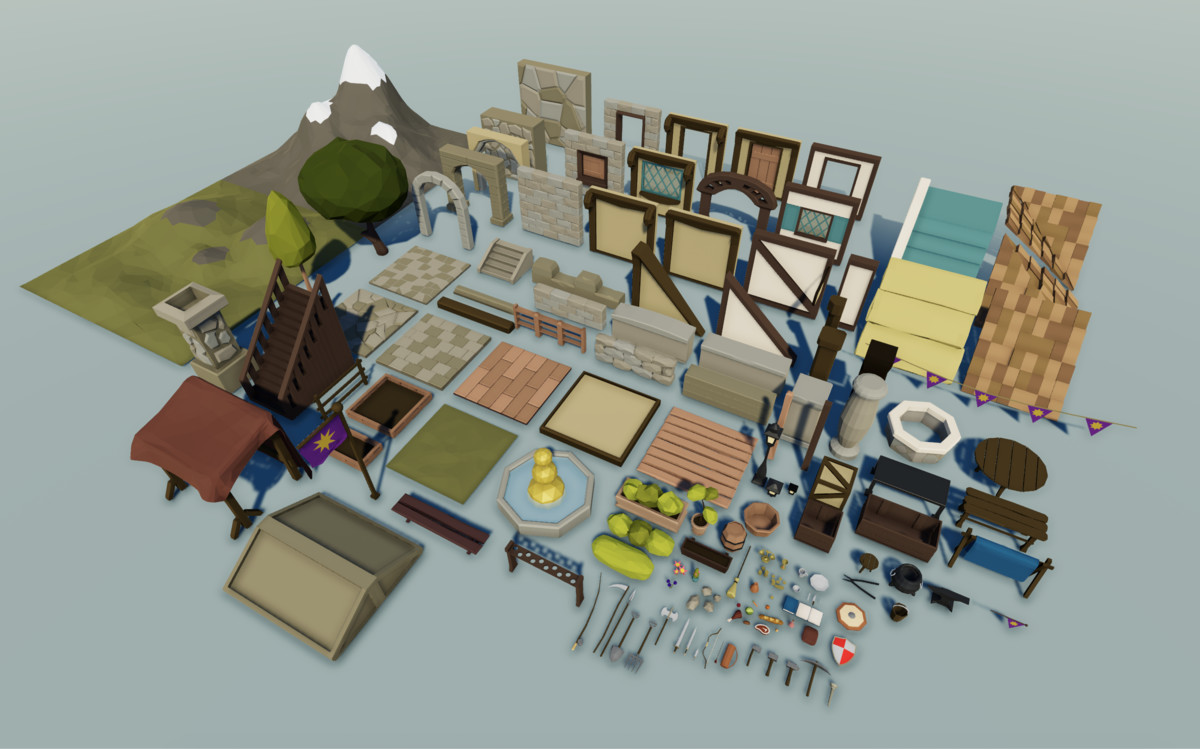
\includegraphics[scale=0.6]{images/village/modular_model_examples.jpg}
\caption{Beispiele für modulare Komponenten zur Modellierung des Dorfes}
\label{fig:modular_model_examples}
\end{figure}

Abbildung \ref{fig:modular_model_examples} zeigt einige Beispiele für modulare Komponenten. Weiterhin ist in Abbildung \ref{fig:modular_house_model_1} ein beispielhaftes Haus zu sehen, das für den Bau des Dorfes aus diesen Komponenten gebildet wurde.

\begin{figure}[H]
\centering
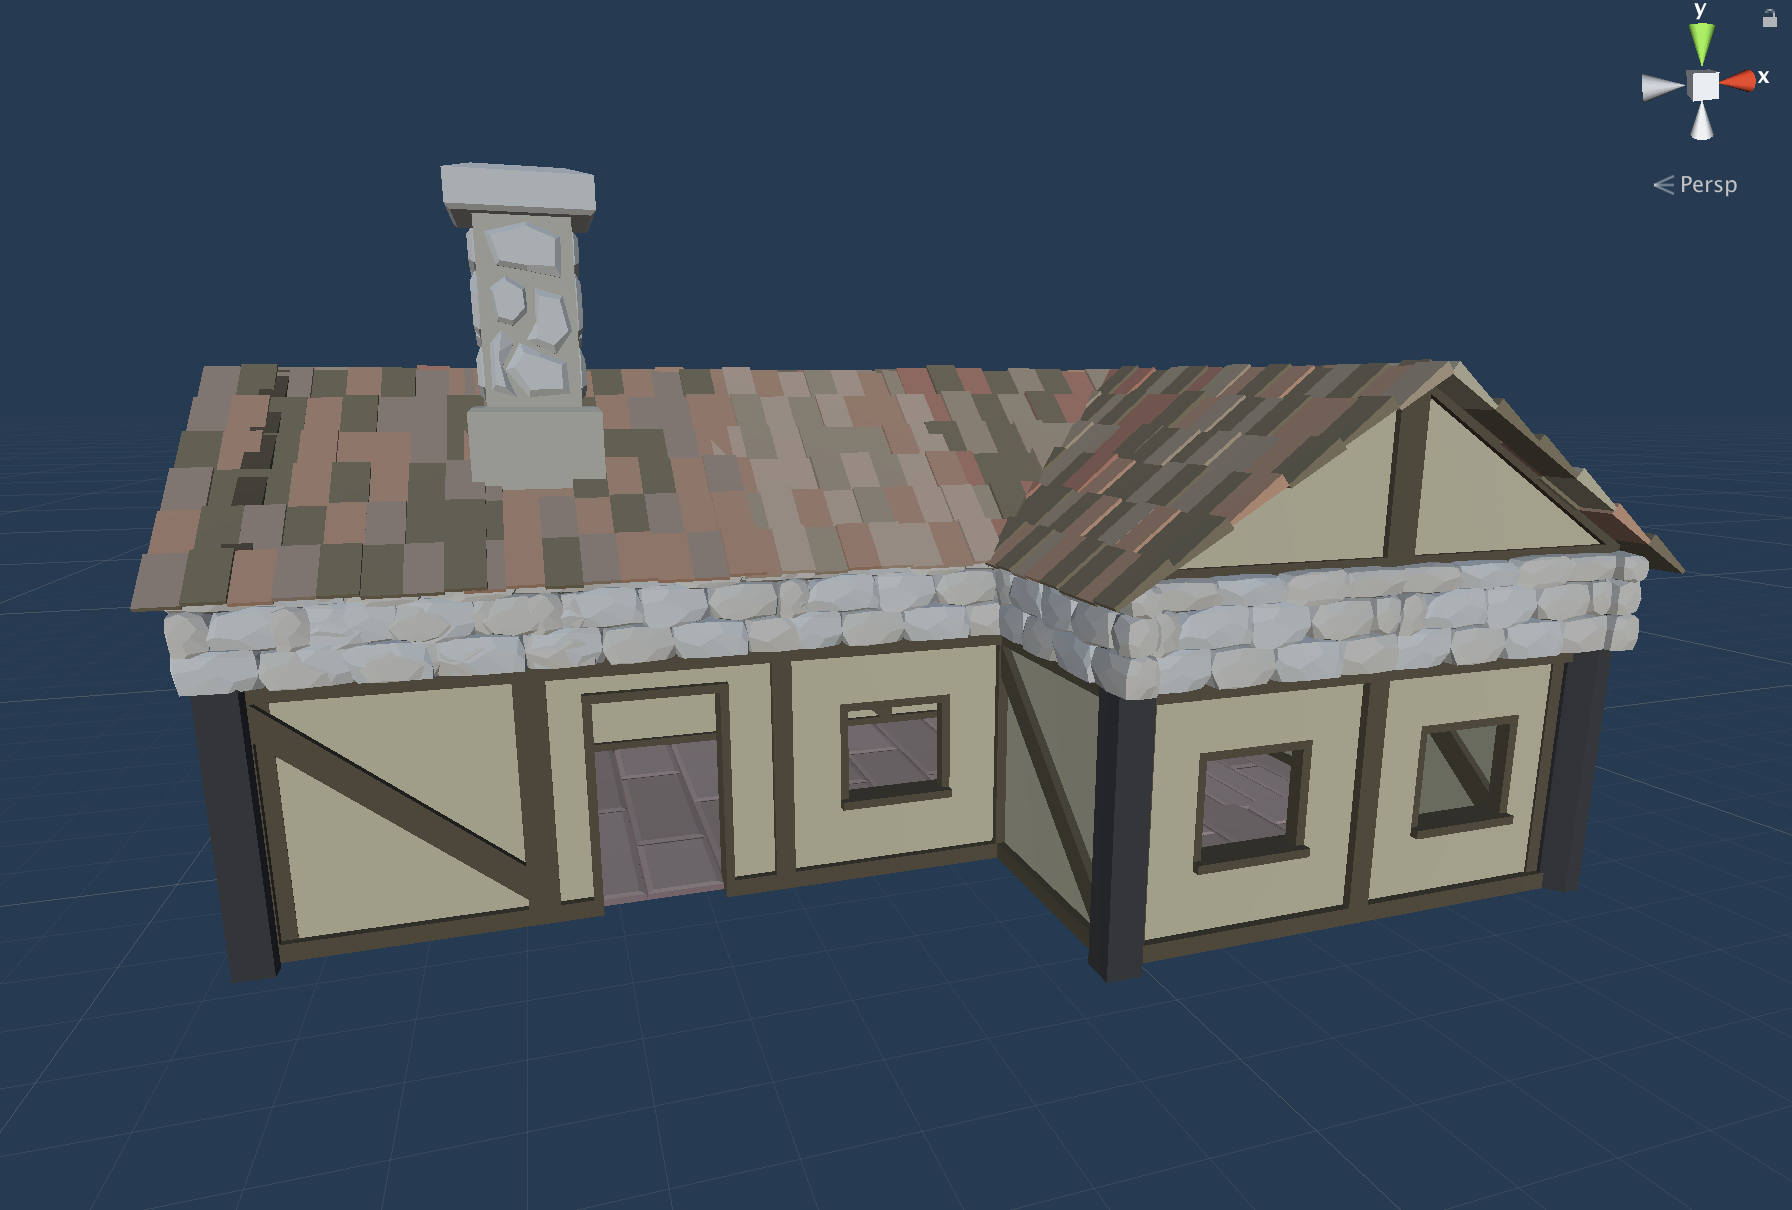
\includegraphics[scale=0.4]{images/village/modular_house_model_1.png}
\caption{Modelliertes modulares Haus}
\label{fig:modular_house_model_1}
\end{figure}

Für Dekorationen, Bäume und Weiteres wurden zusätzlich weitere Sammlungen von Assets verwendet \cite{village_campfire_asset} \cite{village_free_trees_assets} \cite{village_windmill_asset} \cite{village_citypack_asset}.

Die Abbildungen \ref{fig:village_village_day_1} und \ref{fig:village_village_day_2} zeigen die modellierte Stadt mit einer Vielzahl von Gebäuden und Dekorationen wie Bäumen und Zäunen. Auf den Abbildungen sind sowohl eine Außenansicht eines großen Teils der Stadt als auch eine beispielhafte Innenansicht einer Straße zu erkennen. Um eine visuelle Abgrenzung zur Außenwelt vorzunehmen, wurden Felsen um die Stadt herum positioniert, die nicht passierbar sind.

\begin{figure}[H]
\centering
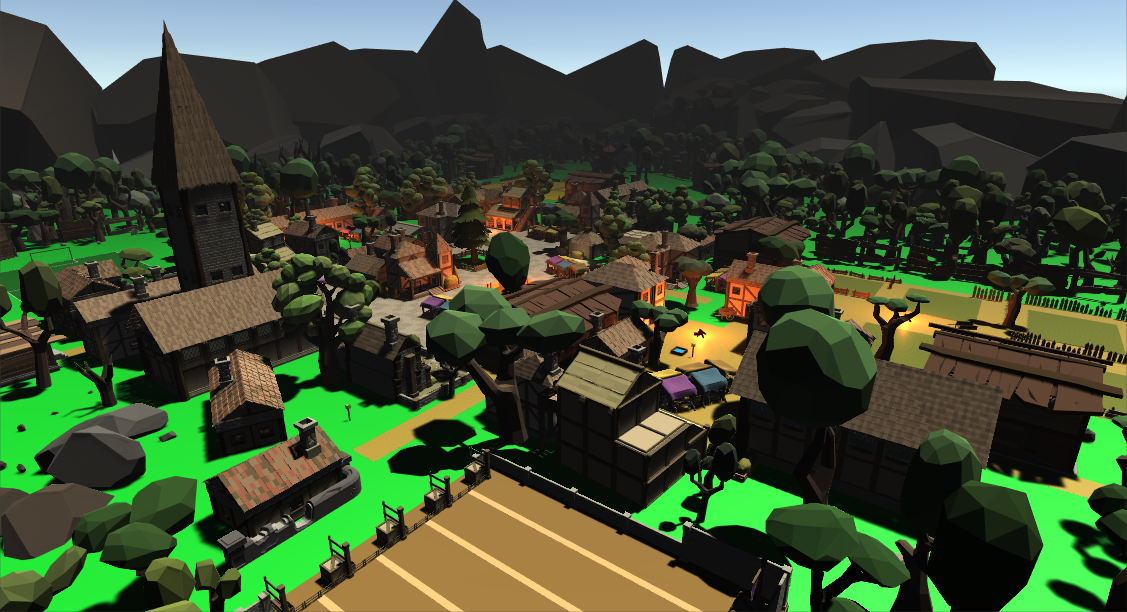
\includegraphics[scale=0.525]{images/village/village_village_day_1.PNG}
\caption{Modellierte Stadt, äußere Ansicht}
\label{fig:village_village_day_1}
\end{figure}

\begin{figure}[H]
\centering
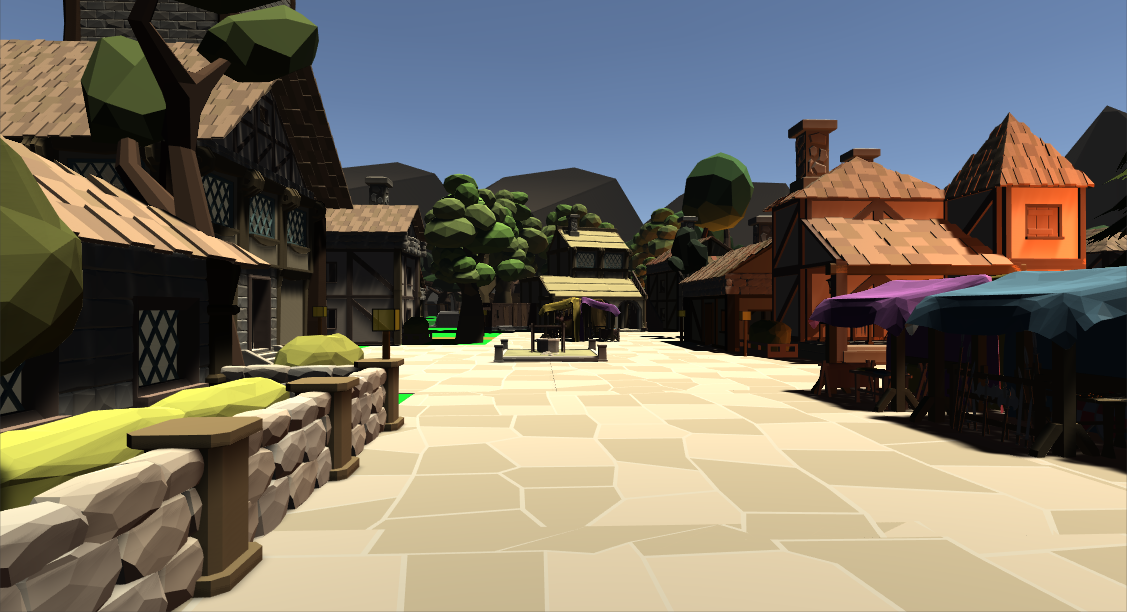
\includegraphics[scale=0.525]{images/village/village_village_day_2.png}
\caption{Modellierte Stadt, innere Ansicht}
\label{fig:village_village_day_2}
\end{figure}
















\section{Softwaredesign- und Architektur}
Im Verlauf dieses Abschnitts wird die Architektur der Simulation erläutert. Zunächst wird hierfür ein genereller Überblick vermittelt, der die grundsätzliche Struktur beschreibt. Anschließend werden die einzelnen Komponenten anhand der zentralen Klassen näher betrachtet und ihre Funktionsweise erläutert. Generell wurde ein objektorientierter Ansatz gewählt. Im Folgenden wird die in Abbildung \ref{fig:architecture_diagram_init_example} verwendete Notation verwendet, um den Aufbau von Klassen anhand der Signaturen ihrer Methoden und Felder zu beschreiben.

\begin{figure}[H]
\centering
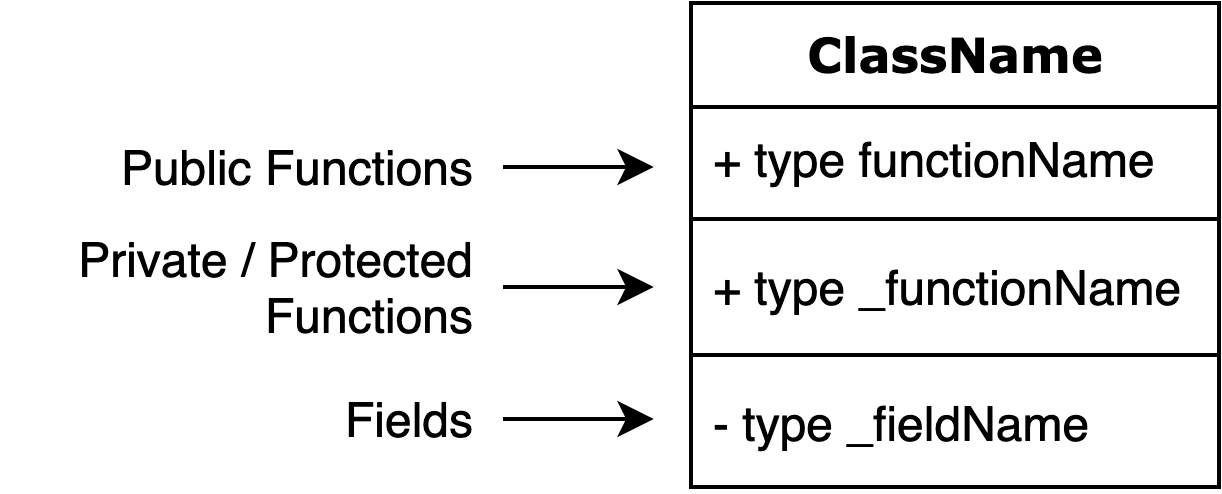
\includegraphics[scale=0.21]{images/village/architecture_diagram_init_example.png}
\caption{Verwendete Notation für die Beschreibung von Klassen}
\label{fig:architecture_diagram_init_example}
\end{figure}

Da das ML-Agents Toolkit verwendet wird, hängt die grundlegende Architektur des Dorfes teilweise von der im Kapitel \ref{ml_unity} erläuterten Struktur ab (siehe \ref{fig:ml-agents_architecture}). Insbesondere betrifft das die Entwicklung der Agenten und Entscheidungen sowie die Ausführung von Aktionen. Daher wird der in Kapitel \ref{ml_unity} vorgestellte Prozess verwendet, der eine \inlinecode{Academy}-Instanz mit mehreren Agenten und bestimmten nötigen Funktionen vorsieht.

\bigskip
\begin{figure}[H]
\centering
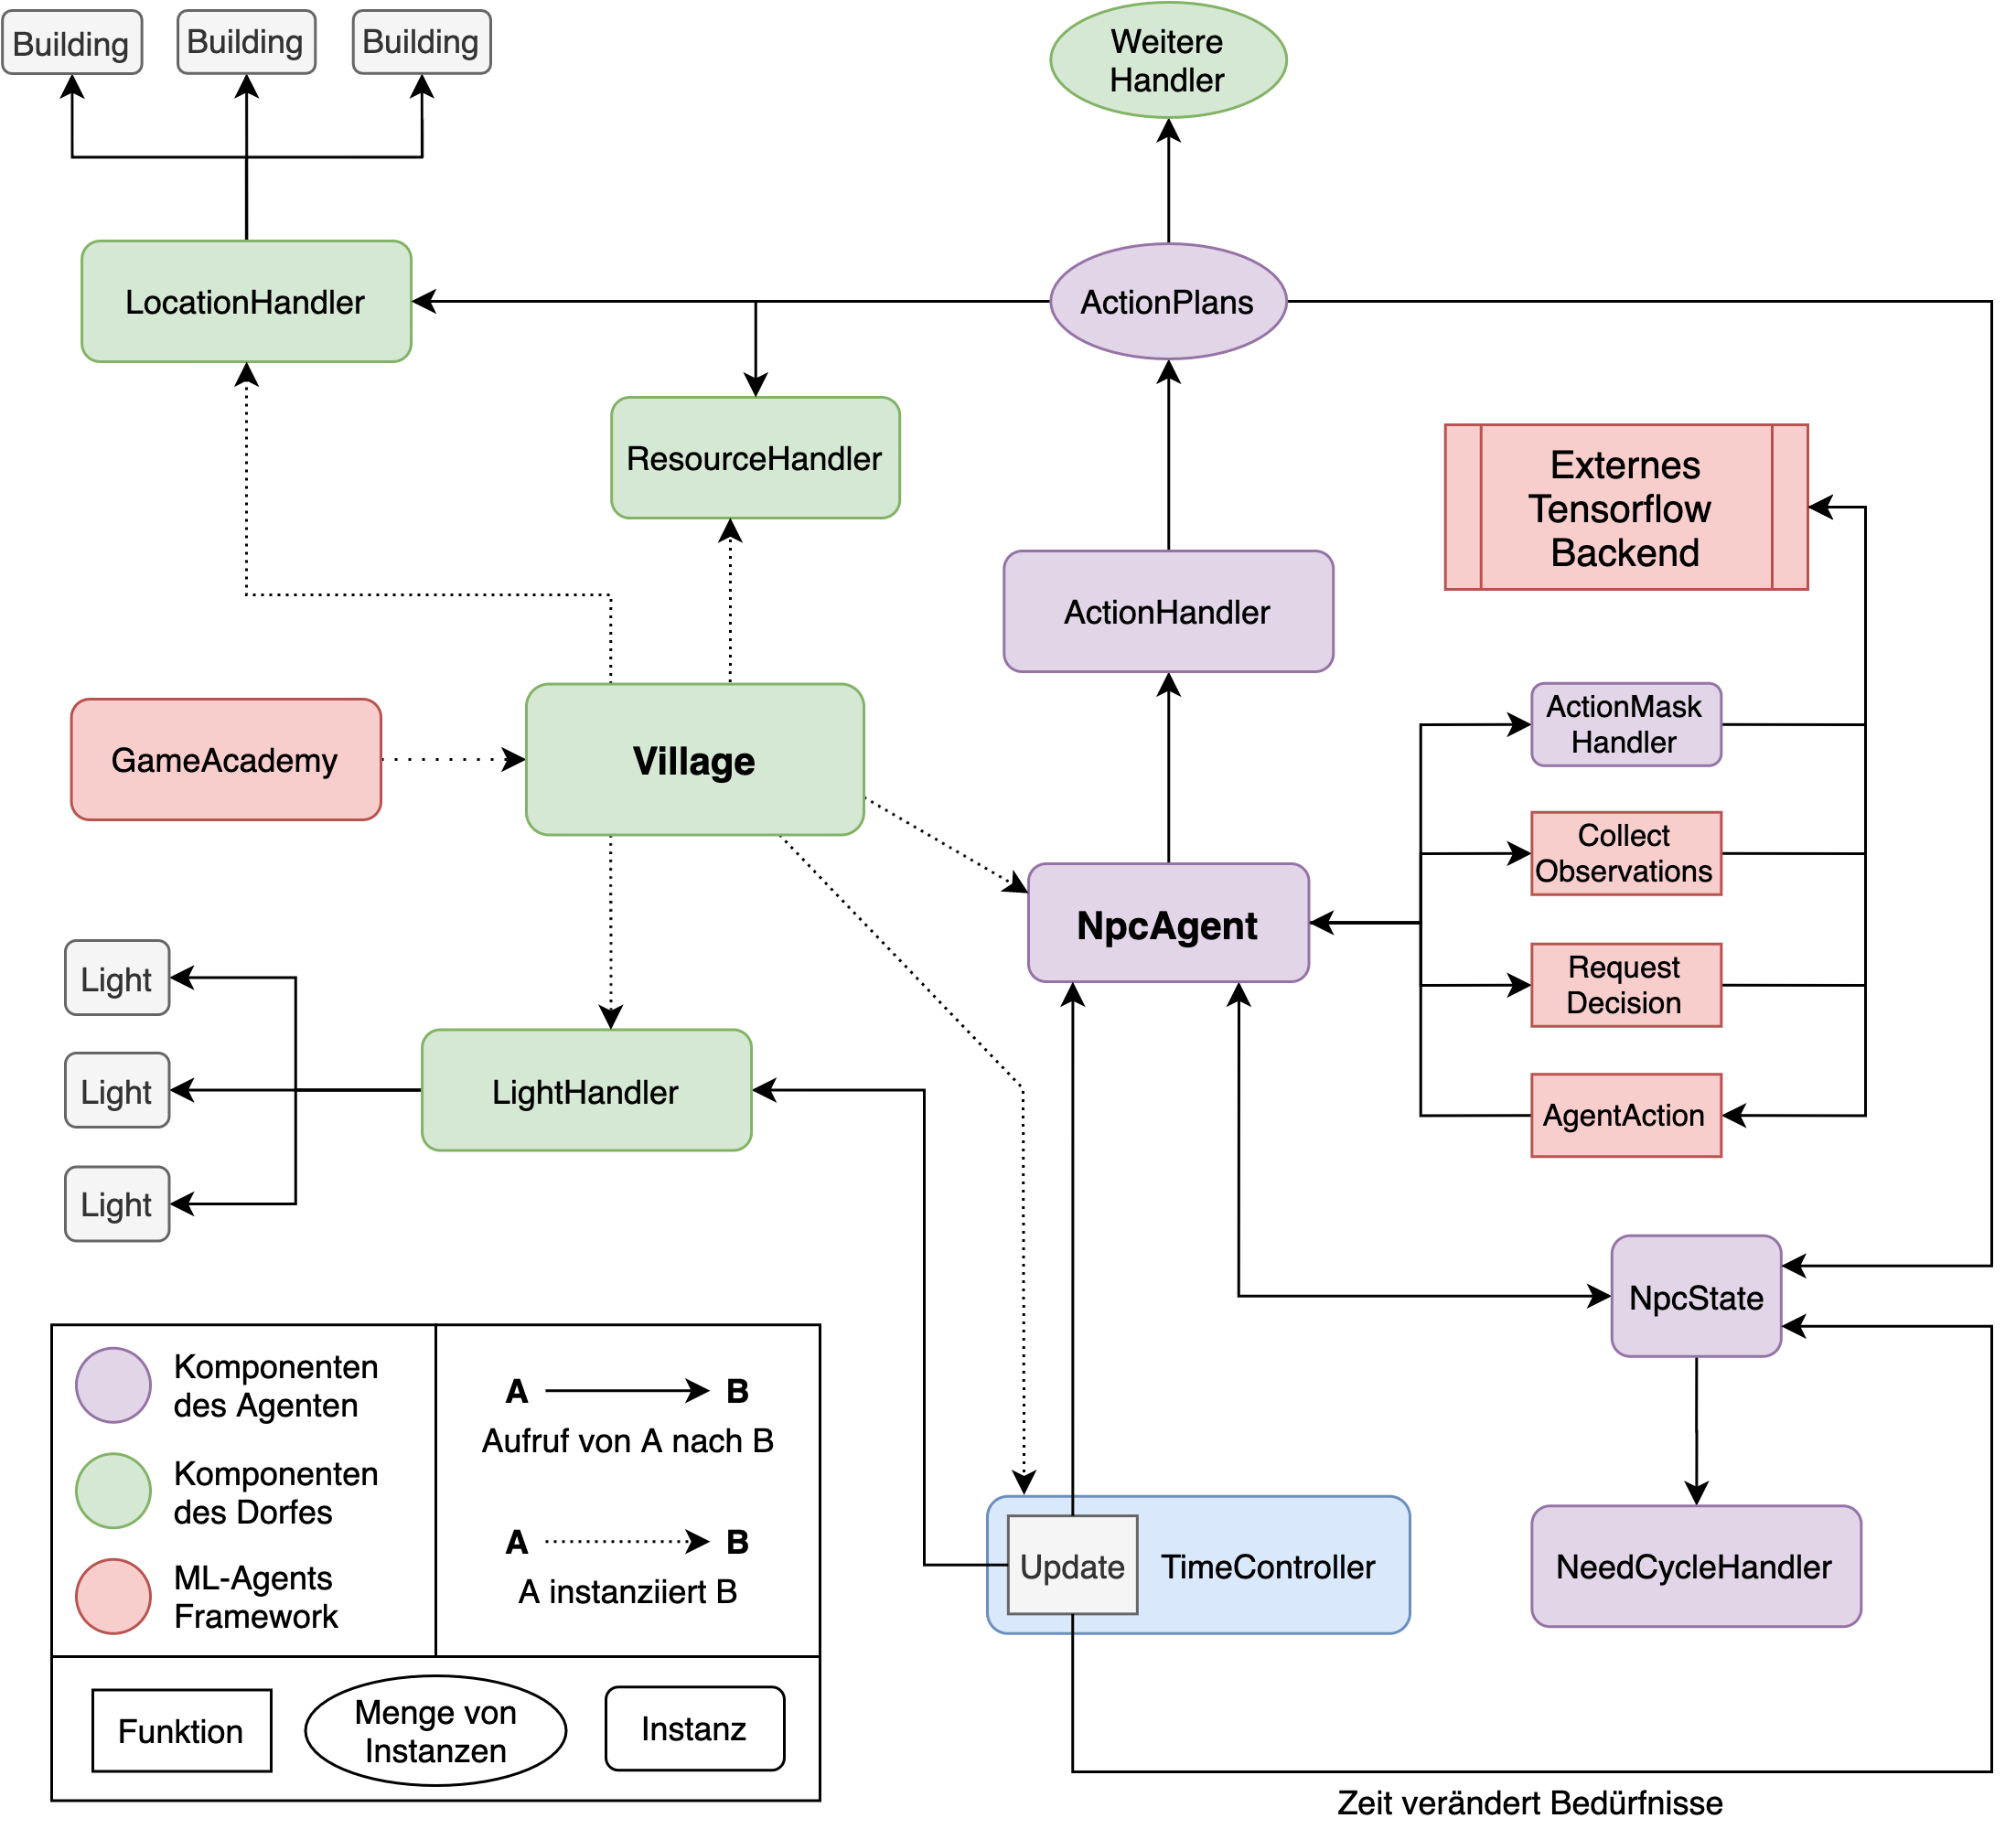
\includegraphics[scale=0.21]{images/village/Master-Thesis_Diagram_Architecture_2.png}
\caption{Grundsätzliche Architektur des Dorfsystems}
\label{fig:architecture_general}
\end{figure}

Abbildung \ref{fig:architecture_general} zeigt den grundsätzlichen Aufbau der Implementierung. Die beiden Komponenten \inlinecode{Village} und \inlinecode{NpcAgent} bilden die zentralen Elemente für den Ausführungskreislauf bzw. \Fachbegriff{Game Loop} der Simulation. Es besteht eine direkte Anbindung zum ML-Agents Toolkit über die \inlinecode{GameAcademy}. Zunächst wird \inlinecode{Village} durch die \inlinecode{GameAcademy} initialisiert. \inlinecode{Village} wiederum erzeugt eine festgelegte Anzahl von Agenten. Es gibt also eine kaskadierte Hierarchie für die Initialisierung der Simulation mit der \inlinecode{GameAcademy} an höchster Stelle, gefolgt von mehreren Instanzen vom Typ \inlinecode{Village} und schließlich jeweils mehreren Instanzen vom Typ \inlinecode{NpcAgent}.

\inlinecode{Village} verfügt über verschiedene Subkomponenten, die für das Steuern bestimmter Aufgaben verantwortlich sind. Über den \inlinecode{ResourceHandler} wird das Ressourcensystem verwaltet, auf das die NPCs zugreifen können. Zusätzlich verwaltet der \inlinecode{LocationHandler} alle Orte im Spiel, zu denen ein Agent navigieren kann. Dazu gehören sämtliche Häuser inklusive deren Räume und weitere Orte außerhalb von Gebäuden. Zuletzt ist der \inlinecode{LightHandler} dafür zuständig, die Tageszeit anhand des Sonnenstandes und der Kontrolle von Lichtquellen zu simulieren.
Der \inlinecode{NpcAgent} erbt von der ML-Agents-Klasse \inlinecode{Agent} und ist somit für das Reinforcement Learning und die Ausführung von Aktionen vorhanden. Das Framework wählt Aktionen für den Agenten aus und stößt diese an. Die Aktionen, die ein Agent ausführen kann, benötigen immer ein Ziel und verwenden daher den \inlinecode{LocationHandler}. Sie beeinflussen außerdem den Zustand \inlinecode{NpcState} eines Agenten. Dieser beinhaltet beispielsweise die Bedürfnisse eines Agenten, die von Aktionen aufgefüllt werden können. Die Funktionen, die die Abnahme der Bedürfnisse bestimmen, werden im \inlinecode{NeedCycleHandler} definiert und werden über diesen aktualisiert. Aktionen können außerdem Ressourcen aufbrauchen oder produzieren, indem der \inlinecode{ResourceHandler} verwendet wird.

Eine zentrale Zeitverwaltungseinheit wird durch den \inlinecode{TimeController} realisiert. Dieser berechnet in regelmäßigen Abständen aufgrund der verstrichenen Zeit die neue Zeit im Spiel. Anschließend werden alle Komponenten, für die das Voranschreiten der Zeit relevant ist, mit dieser neuen Zeit versorgt. Der \inlinecode{LightHandler} regelt mit dessen Hilfe beispielsweise die Intensität und Position der Sonne wohingegen der \inlinecode{NeedCycleHandler} aufgrund der verstrichenen Zeit die neuen Bedürfnisse des Agenten berechnet und den \inlinecode{NpcState} entsprechend anpasst.



\section{Implementierung}
In den folgenden Abschnitten werden die wichtigsten Klassen der Dorfsimulation im Einzelnen erläutert. Zunächst werden dafür die zentralen, übergeordneten Komponenten \inlinecode{Village} und \inlinecode{GameAcademy} näher betrachtet.


\subsection{Village}
Die Aufgabe der Komponente \inlinecode{Village} ist die Erzeugung von \acp{npc} und die Bereitstellung einer zentralen Verwaltungseinheit für Komponenten. Abbildung \ref{fig:architecture_diagram_village} zeigt den Aufbau der Klasse \inlinecode{Village} anhand ihrer Funktionen:

\begin{figure}[H]
\centering
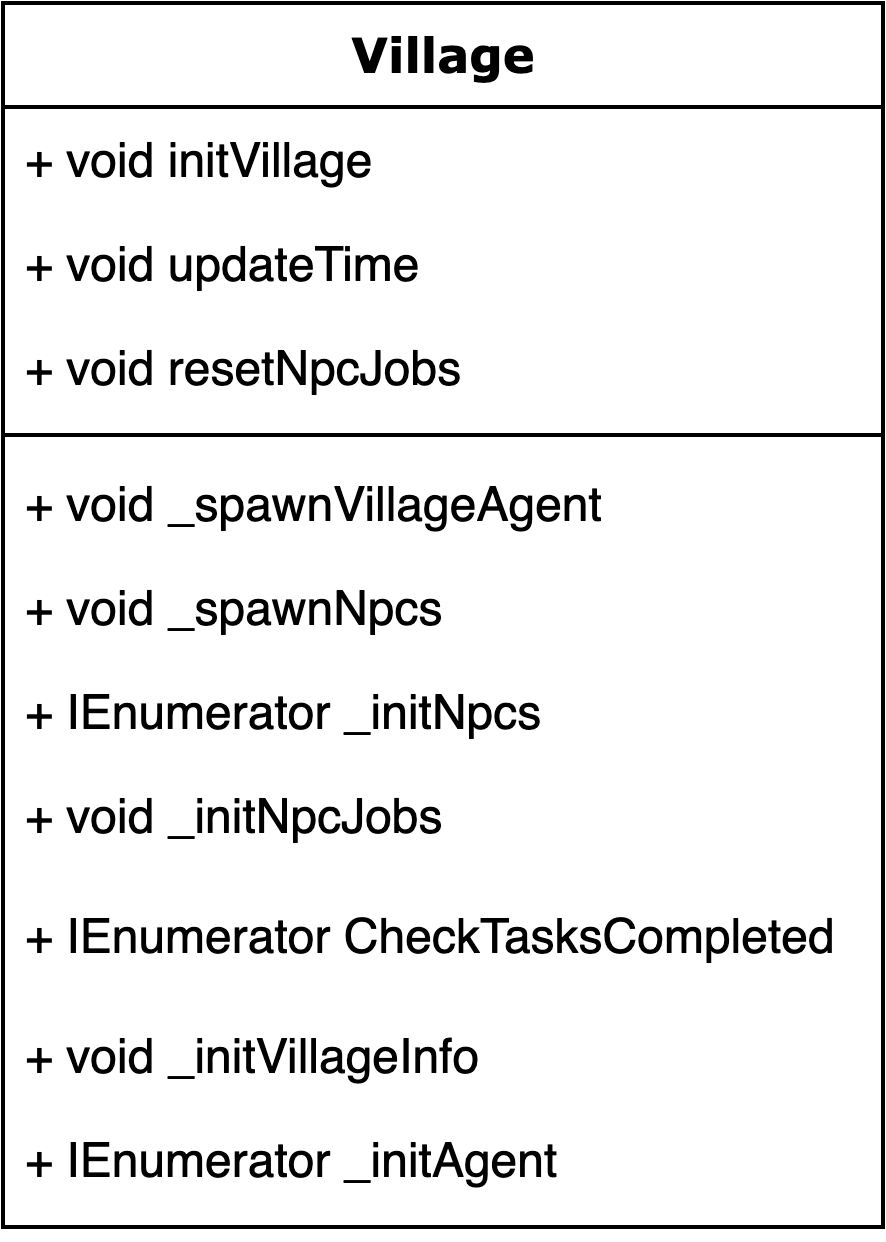
\includegraphics[scale=0.18]{images/village/architecture_diagram_village.png}
\caption{Methoden der Klasse \inlinecode{Village}}
\label{fig:architecture_diagram_village}
\end{figure}

\inlinecode{Village} erzeugt und initialisiert zunächst Handler-Klassen wie \inlinecode{TimeController}, \inlinecode{LocationHandler}, \inlinecode{ResourceHandler} und \inlinecode{LightHandler} in der Funktion \inlinecode{initVillage}. Anschließend werden weitere Funktionen aufgerufen, um innerhalb von Coroutinen asynchron Agenten zu erzeugen. Diese werden in \inlinecode{\_spawnNpcs} zunächst erstellt und dann in \inlinecode{\_initNpcs} initialisiert, wie in Listing \ref{lst:village_init_npcs} zu sehen.

\begin{minipage}{\linewidth}
\begin{lstlisting}[linewidth=16.4cm, label=lst:village_init_npcs, caption=Initialisierung von Agenten, xleftmargin=1cm]
private IEnumerator _initNpcs() {
    _npcLoadingTasks = new Dictionary<int, bool>();
    for (int i = 0; i < _villageNpcs.Count; i++) {
        _npcLoadingTasks[i] = false;
        _villageNpcs[i].StartCoroutine(_initAgent(i));
    }
    yield return StartCoroutine(CheckTasksCompleted());
    _villageAgent.init(this);
    GameAcademy.NPC_LOADING_DONE = true;
}
\end{lstlisting}
\end{minipage}

Für jeden Agenten wird eine einzelne Coroutine \inlinecode{\_initAgent} gestartet. Anschließend wird mit \inlinecode{yield return} auf die Ausführung einer weiteren Coroutine \inlinecode{CheckTasksCompleted} gewartet, die in bestimmten Abständen prüft, ob die weiteren Coroutinen beendet wurden.

Mit der Funktion \inlinecode{\_spawnVillageAgent} wird darüber hinaus die Klasse \inlinecode{VillageAgent} initialisiert (siehe Abschnitt \ref{village_village_agent}). Sobald alle \inlinecode{NpcAgent}s erfolgreich initialisiert wurden, wird auch der \inlinecode{VillageAgent} initialisiert.

\inlinecode{Village} speichert Referenzen auf alle Agenten \inlinecode{NpcAgent} des Dorfes und bietet eine Schnittstelle für weitere Komponenten, um Zugriff auf die Agenten zu erlangen. Zusätzlich verfügt das Dorf über eine Instanz der Klasse \inlinecode{VillageInfo}, die in der Methode \inlinecode{\_initVillageInfo} erzeugt wird. Darin werden Informationen über den aktuellen Zustand des Dorfes gespeichert. Dazu gehört beispielsweise die Anzahl der Agenten, die aktuell eine bestimmte Aktion ausführen. Diese Daten werden anschließend im UI der Simulation dargestellt. Aus diesem Grund verfügt \inlinecode{VillageInfo} über eine Vielzahl von Tracking-Funktionen, die diese Statistiken verwalten.




\subsection{GameAcademy}\label{gameacademy}
Die \inlinecode{GameAcademy} erbt von der ML-Agents Basisklasse \inlinecode{Academy} (siehe Kapitel \ref{ml_unity}) und erweitert diese um verschiedene Einstellungsmöglichkeiten sowie dem Ladevorgang des Dorfes. In Abbildung \ref{fig:architecture_diagram_gameacademy} wird der Aufbau der Klasse verdeutlicht:

\begin{figure}[H]
\centering
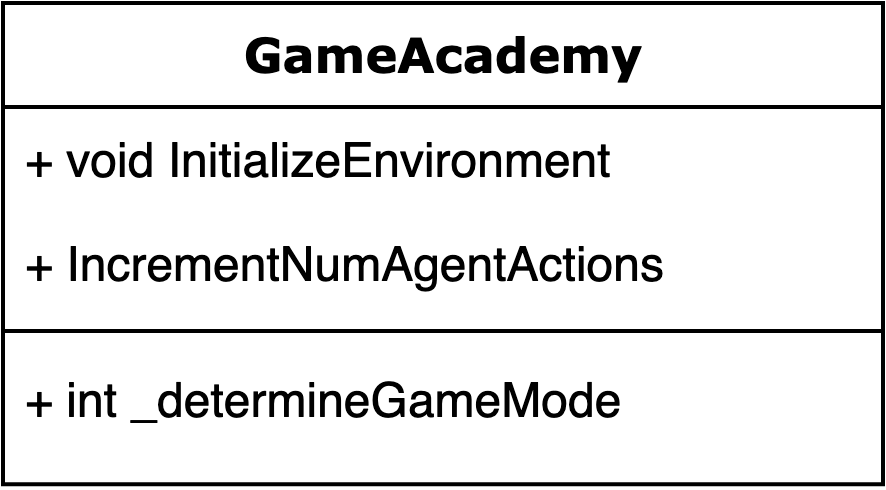
\includegraphics[scale=0.18]{images/village/architecture_diagram_gameacademy.png}
\caption{Methoden der Klasse \inlinecode{GameAcademy}}
\label{fig:architecture_diagram_gameacademy}
\end{figure}

Zunächst wird die Funktion \inlinecode{InitializeEnvironment} durch \inlinecode{ML-Agents} aufgerufen. Hier werden zunächst einige Parameter ausgewertet, die über den Unity Editor gesetzt werden können. Neben den Parametern der Oberklasse \inlinecode{Academy} können hier für die Simulation grundlegende Einstellungen vorgenommen werden, wie die Anzahl der zu erzeugenden NPCs oder die Auswahl des Inference-Modus zwischen den unterschiedlichen implementierten Verfahren wie beispielsweise Reinforcement Learning oder GOAP. Für jeden dieser Parameter existiert eine statische Variable, die von allen verwendeten Komponenten innerhalb des Dorfes einfach gelesen werden kann.
Aufgrund dieser Parameter sowie dem Rückgabewert von \inlinecode{GetIsInference} wird in der Funktion \inlinecode{\_determineGameMode} anschließend eine weitere Variable gesetzt, die den Spielmodus festlegt. Bestimmte Komponenten verhalten sich je nach Spielmodus auf eine andere Art und Weise (siehe Abschnitt \ref{modes_fake_inference_etc}).

Alle Komponente vom Typ \inlinecode{Village} werden anschließend durch die Anweisung \inlinecode{FindObjectsOfType<Village>()} hinzugefügt. Die \inlinecode{GameAcademy} startet dann den Ladevorgang der Simulation, indem alle Instanzen von \inlinecode{Village} initialisiert werden. Mehrere Dörfer mit jeweils einem \inlinecode{Village}-Modul können gleichzeitig verwendet werden, indem das Prefab für das Spielfeld dupliziert wird.

Die Funktion \inlinecode{IncrementNumAgentActions} ist ausschließlich für den \inlinecode{VillageAgent} relevant und wird im Abschnitt \ref{village_village_agent} behandelt.

Die in Tabelle \ref{tab:game_academy_parameters} zu sehenden Parameter können in der \inlinecode{GameAcademy} angepasst werden. Die Tabelle enthält für jeden Parameter eine kurze Beschreibung, die aus den entsprechenden Kommentaren im Programmcode entnommen wurden.

\smallskip
\begin{table}[H]
\footnotesize
\centering
\begin{tabular} {|  p{4.2cm}  |  p{11.4cm}  |} \hline
\textbf{Parameter} & \textbf{Beschreibung} \\ \hline

\inlinecode{numAgentsPerVillage25} & Define how many agents should be spawned per village. This should be in order of 25s (25, 50, 75...), for the jobs distribution to work properly. \\ \hline
\inlinecode{actionsPerAgentUntilReset} & Define how many decisions the agents should perform until they are reset. \\ \hline
\inlinecode{debugMode} & Tracks some additional data useful for debugging when activated. \\ \hline
\inlinecode{useFakeInference} & Since high timescale levels do not scale well with NavMeshAgents, a kind of fake inference will have to be used, in which agents teleport to their destinations and additionally wait for an amount of time that is equal to the time it would have taken to move there. \\ \hline
\inlinecode{verbose} & Prints some additional information when activated. \\ \hline
\inlinecode{actionsUntilVillageAction} & Decides how many steps will be performed per agent between VillageAgent decisions. \\ \hline
\inlinecode{villageDecisionsReset} & Decides how many decisions will be made by the VillageAgent until Done is called. \\ \hline
\inlinecode{useManualNpcDecisions} & Uses manual decisions instead of the trained model. \\ \hline
\inlinecode{ignoreVillageAgent} & Ignores the village agent and sticks with the initial distribution of jobs. \\ \hline
\inlinecode{useGoap} & Uses GOAP agents instead of a trained model. \\ \hline
\inlinecode{agentStoppingDistance} & Determines how far from his target an agent will stop when moving to a destination. \\ \hline
\inlinecode{agentRythmVariation} & Decides the amount of variation between the day/night cycles of the agents. \\ \hline
\inlinecode{logActionDurations} & Determines whether the duration of actions should be tracked in VillageInfo. \\ \hline
\inlinecode{logRewards} & Determines whether the rewards should be tracked for each action to gain some statistical information. \\ \hline
\inlinecode{logNeeds} & Logs the average needs of NPCs at certain times for later analysis. \\ \hline
\inlinecode{logAttributes} & Logs the average attributes of agents for each action. \\ \hline
\inlinecode{logActionMaskAmounts} & Determines whether to log the amount of actions that are masked respectively. \\ \hline
\inlinecode{ignoreAllResources} & Completely ignores all resource handling when set to true. \\ \hline
\inlinecode{ignoreJobMask} & Ignores the job that has been designated to an angent and instead doesn't mask jobs. \\ \hline


\end{tabular}
\caption{Konfigurierbare Parameter der \inlinecode{GameAcademy}}
\label{tab:game_academy_parameters}
\end{table}




\subsubsection{Nutzung mehrerer Villages}
Die Simulation ist nicht auf die Nutzung eines einzelnen Dorfes limitiert. Tatsächlich kann die Verwendung mehrerer Dörfer für den Trainingsvorgang vorteilhaft sein. Aus diesem Grund wurden sämtliche Komponenten so entwickelt, dass mehrere Dörfer reibungsfrei parallel betrieben werden. Zwar beeinflusst dies massiv die Performance des Testsystems, jedoch können dadurch deutlich mehr Agenten verwendet werden - bei der Verwendung eines einzelnen Dorfes würden die Kapazitäten der Gebäude sonst schnell überschritten werden. Weiterhin können dadurch Erfahrungen gesammelt werden, die diverser sind, da die Zustände der Umgebung in unterschiedlichen Dörfern voneinander abweichen.

Zur Verwendung mehrerer Dörfer muss das Prefab des Spielfeldes, das unter anderem das gesamte Mesh beinhaltet, dupliziert werden. Es ist wichtig, dass die Position des Prefabs verändert wird, damit keine Überschneidungen entstehen. Weiterhin sollten alle vorberechneten Daten wie Lichtinformationen oder das NavMesh (siehe Abschnitt \ref{agent_navigation} erneut berechnet werden.
Die \inlinecode{GameAcademy} ist unter anderem für die Initialisierung der Dörfer zuständig. Sie sucht nach allen \inlinecode{Village}-Komponenten in der gesamten Spielszene. Wie in Abbildung \ref{fig:architecture_villages_loading} erkennbar, werden die Dörfer einzeln und unabhängig voneinander geladen. Die Pfeile in der Grafik geben an, welche Klassen durch welche Komponenten instanziiert werden. Das gesamte Ökosystem eines Dorfes, inklusive der Ausführung von Aktionen, verläuft vollkommen unabhängig. Jedes Dorf stellt eine in sich gekapselte Einheit dar, die mit der Außenwelt innerhalb der Simulation, also mit anderen Dörfern, nicht kommuniziert. Jedes Dorf verfügt also über eigene Komponenten wie \inlinecode{ResourceHandler}, \inlinecode{LocationHandler} oder \inlinecode{Village}.

\bigskip
\begin{figure}[H]
\centering
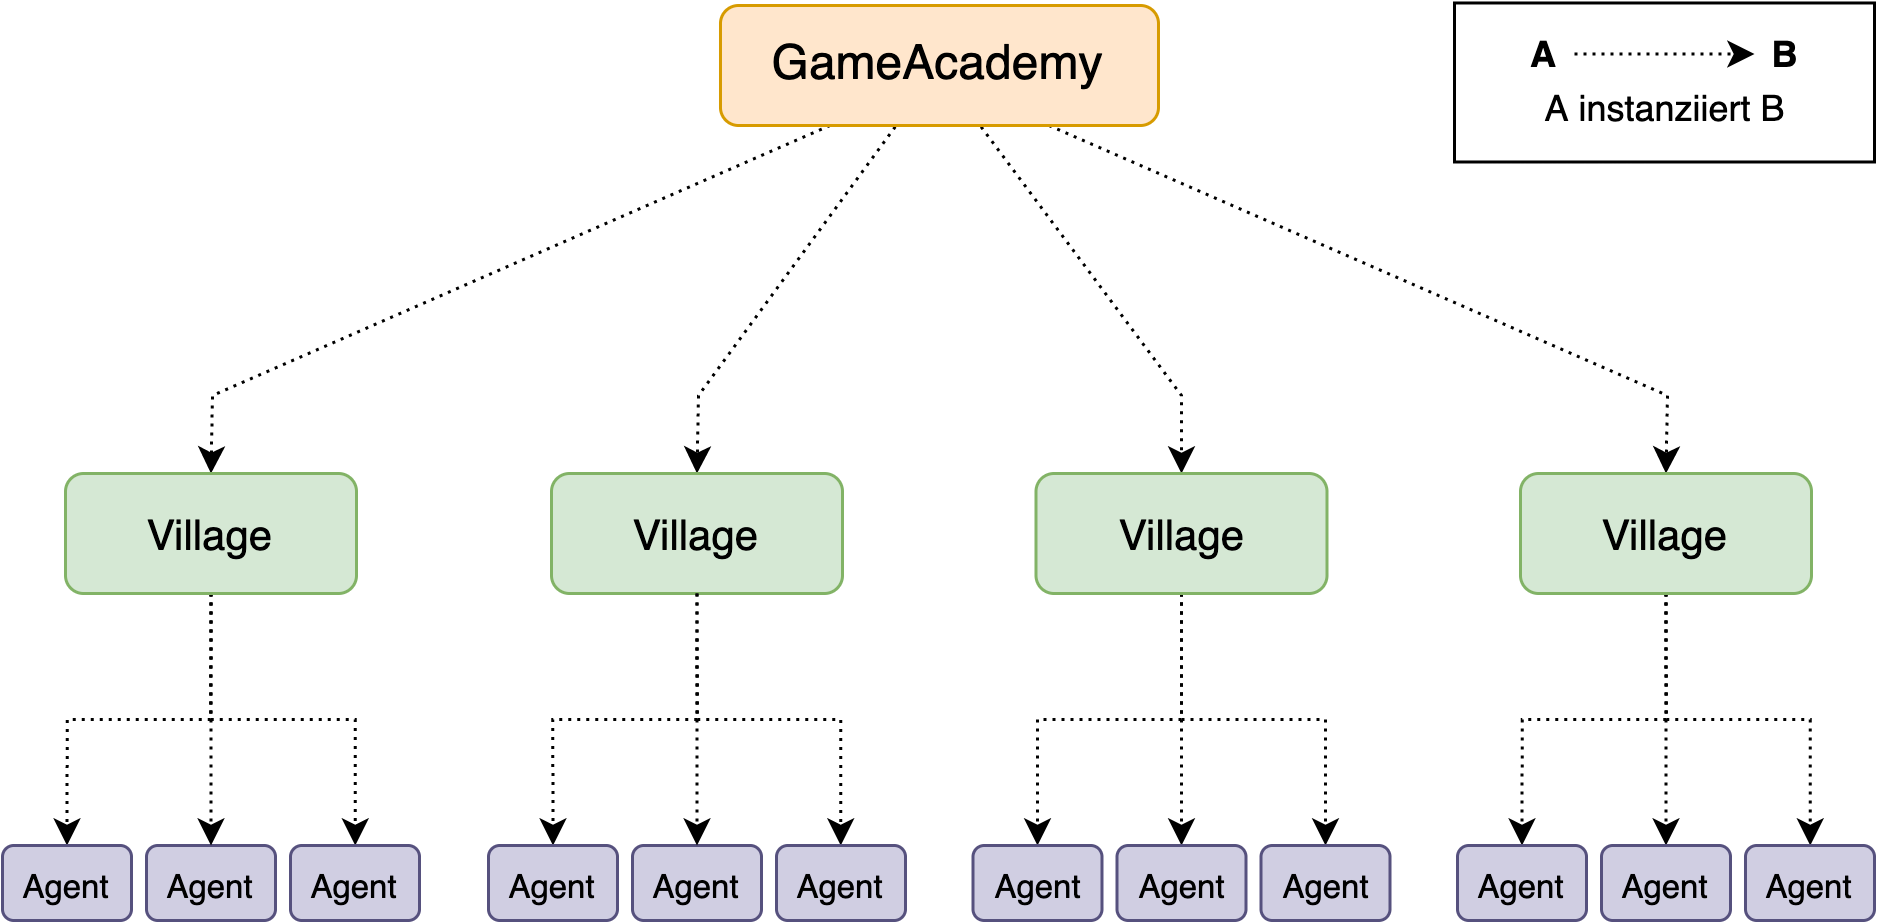
\includegraphics[scale=0.22]{images/village/Master-Thesis_Diagram_Architecture_1.png}
\caption{Architektur, Ladevorgang mehrer Dörfer}
\label{fig:architecture_villages_loading}
\end{figure}





% was verwaltet das dorf alles?

\subsection{LocationHandler}
Die Klasse \inlinecode{LocationHandler} kennt alle im Spiel verfügbaren Gebäude und Orte und bietet allen Agenten eine Schnittstelle, um mit diesen zu interagieren. Er ermöglicht somit neben der benötigten Navigation ebenfalls das Abfragen von Informationen zu bestimmten Gebäudetypen. Die Gebäude haben jeweils eine begrenzte Kapazität, es kann sich also nur eine bestimmte Anzahl von NPCs gleichzeitig in einem Haus befinden. Daher kümmert der \inlinecode{LocationHandler} sich weiterhin um die Verwaltung dieser verfügbaren \inlinecode{Slots}. Der \inlinecode{LocationHandler} wird ausdrücklich nicht für die eigentliche Navigation der Agenten verwendet, stattdessen werden lediglich Orte verwaltet und Positionen zurückgegeben.
Der \inlinecode{LocationHandler} wird durch die Klasse \inlinecode{Village} erzeugt. Abbildung \ref{fig:architecture_diagram_locationhandler} beschreibt den Aufbau.

\begin{figure}[H]
\centering
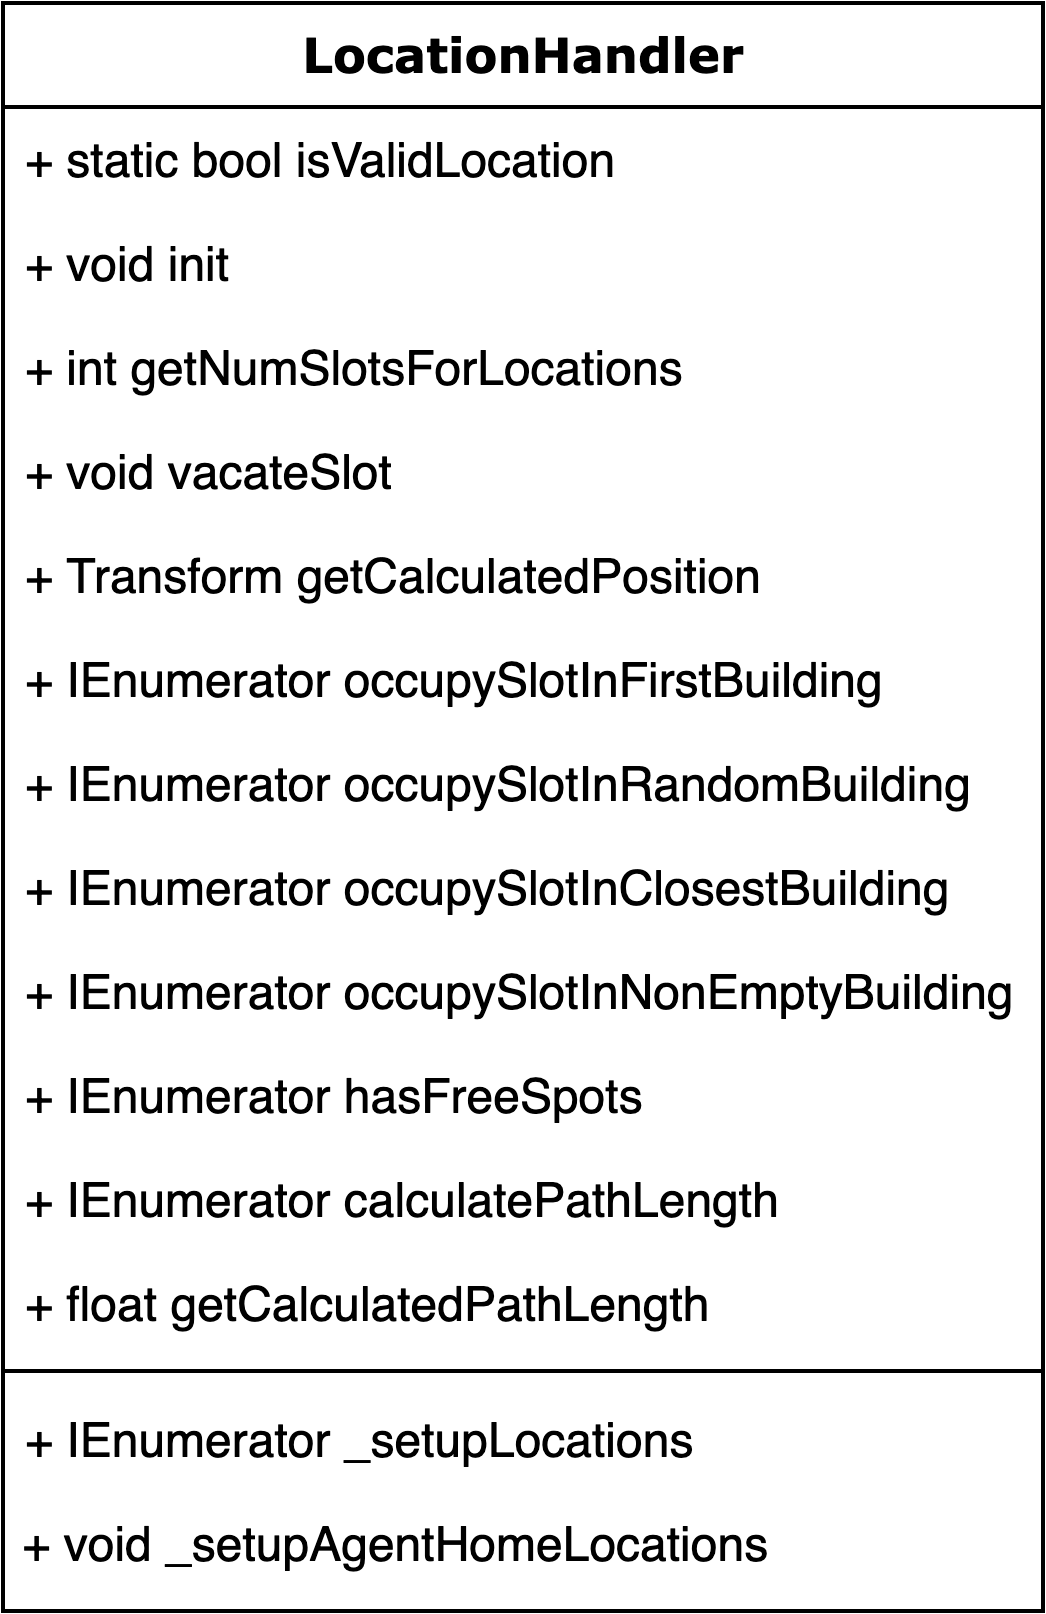
\includegraphics[scale=0.18]{images/village/architecture_diagram_locationhandler.png}
\caption{Methoden der Klasse \inlinecode{LocationHandler}}
\label{fig:architecture_diagram_locationhandler}
\end{figure}

Nach der Initialisierung durch \inlinecode{init} wird zunächst allen Agenten in der Funktion \inlinecode{\_setupAgentHomeLocations} ein Heim zugewiesen, in dem sie wohnen. In der Funktion \inlinecode{\_setupLocations} werden weiterhin alle Gebäude abhängig von ihrem Typ in einem Assoziativen Array gespeichert. in C\# wird dafür typischerweise ein \inlinecode{Dictionary} verwendet, daher ein Feld vom Typen \inlinecode{Dictionary<string, List<Building> >} genutzt. Die verschiedenen Gebäudetypen werden in der Klasse \inlinecode{LocationTypes} definiert, beispielsweise \inlinecode{FIELD\_GRAIN}, \inlinecode{BAKERY} oder \inlinecode{SCHOOL}. Diese werden als Schlüssel verwendet. Die Werte des Dictionary enthalten Listen von Gebäuden (\inlinecode{List<Building>}). Wenn der \inlinecode{LocationHandler} initialisiert wird, werden alle Gebäude des Dorfes gesucht und in die jeweilige Kategorie sortiert. Diese Suche wird beschleunigt, indem alle Gebäude mit einem Tag versehen werden.
Jedes Gebäude und jeder navigierbare Ort in der Stadt verfügt über die Komponente \inlinecode{Building}. In jedem Gebäude-Prefab werden sogenannte \inlinecode{BuildingNavPoint}s definiert, welche die tatsächlichen Orte bzw. \Fachbegriff{Slots} darstellen, zu denen die Agenten navigieren können. Dafür werden Objekte erstellt, die eine Position innerhalb des Gebäudes zugewiesen bekommen. Diesen wird die Komponente \inlinecode{BuildingNavPoint} angefügt. Die Menge der \inlinecode{BuildingNavPoint} in einem Gebäude bestimmt die Kapazität des Gebäudes. \inlinecode{BuildingNavPoint} können von nur einem NPC zur Zeit durch den Aufruf der Funktion \inlinecode{occupy} besetzt werden und müssen, sobald der Agent den Ort verlässt, anschließend durch die Funktion \inlinecode{vacate} wieder geräumt werden. Zusätzlich wird ein \inlinecode{DistanceNavPoint} definiert. Dieser wird verwendet, um die Distanz des Agenten zu einem bestimmten Gebäude zu ermitten und befindet sich daher im Eingang des Gebäudes. Falls es mehrere Eingänge gibt, wird die Mitte des Hauses gewählt. Die Abbildung \ref{fig:village_navpoints} zeigt beispielhaft, wie \inlinecode{BuildingNavPoint} und der \inlinecode{BuildingDistanceNavPoint} in einem beispielhaften Gebäude definiert werden. Zur besseren Darstellung wurde jedem \inlinecode{BuildingNavPoint} ein Mesh in Form von einer Kugel zugewiesen, die normalerweise deaktiviert ist. Für die Platzierung der Objekte kann dieses Mash aktiviert werden.

\begin{figure}[H]
\centering
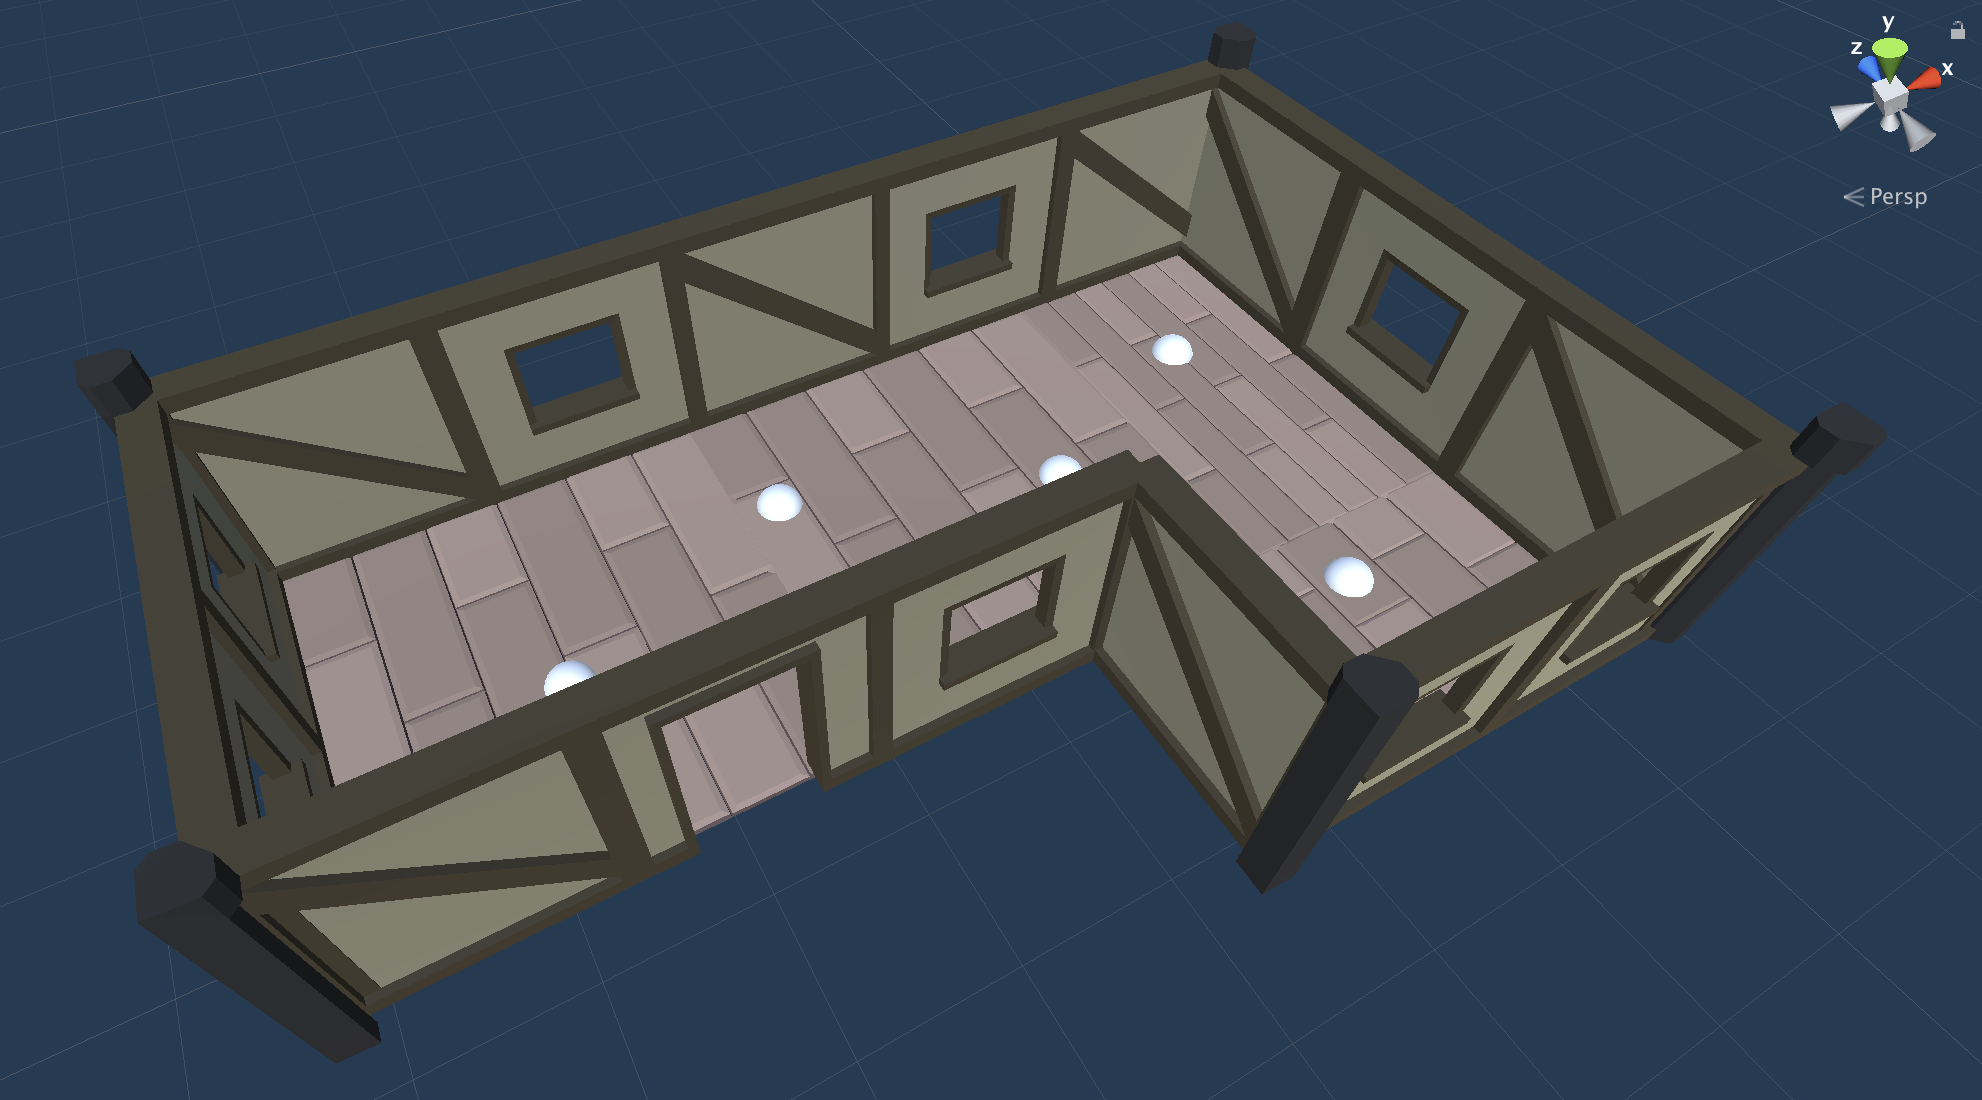
\includegraphics[scale=0.35]{images/village/village_navpoints_example.png}
\caption{Definition von \inlinecode{BuildingNavPoints} und \inlinecode{BuildingDistanceNavPoint}}
\label{fig:village_navpoints}
\end{figure}

\inlinecode{Building} enthält alle \inlinecode{BuildingNavPoint} des Gebäudes und verwaltet diese. Es werden Referenzen auf die bereits besetzten Slots in Gebäuden sowie den jeweiligen NPCs gehalten. Weiterhin ist für jeden Typ aus \inlinecode{LocationTypes} bekannt, wie viele offene Slots noch vorhanden sind.
Der \inlinecode{LocationHandler} bietet nun eine Menge von Funktionen. Diese stellen allesamt NPCs Orte zur Verfügung, unterscheiden sich jedoch leicht in ihrer Semantik:
\begin{itemize}
    \item \inlinecode{occupySlotInFoundBuilding} findet das erste Gebäude eines bestimmten Typs, das einen freien Slot hat und gibt die Position des ersten Slots in dem Gebäude zurück.
    \item \inlinecode{occupySlotInRandomBuilding} wird genutzt, um ein zufälliges Gebäude mit einem zufälligen Slot auszuwählen.
    \item \inlinecode{occupySlotInClosestBuilding} soll das nicht besetzte Gebäude finden, das sich von der Position des Agenten örtlich am wenigstens weit weg entfernt befindet.
    \item \inlinecode{occupySlotInNonEmptyBuilding} findet das erste Gebäude, das bereits mit mindestens einem Agenten besetzt ist. Falls kein Gebäude gefunden wird, wird eine zufällige Position zurückgegeben. Die Funktion wird unter anderem verwendet um zu simulieren, dass sich mehrere Agenten auf einem Marktplatz treffen, um miteinander zu kommunizieren. In diesem Fall wird stets ein Ort zurückgegeben, der bereits von einem \ac{npc} beansprucht wird, sodass diese sich \sogenannt{treffen} können und Gruppen entstehen.
\end{itemize}

Die Funktion \inlinecode{occupyFreeSlotInRandomBuilding} wird beispielhaft in Listing \ref{lst:village_location-handler_example} aufgeführt. Zunächst wird für alle Gebäude des Typs geprüft, ob sie über freie Plätze verfügen. Für diese Gebäude wird dessen Index in einer Liste gespeichert. Aus dieser Liste wird nun ein zufälliger Index \inlinecode{randomIndex} ausgewählt, der bestimmt, zu welchem Ort der Agent navigieren wird. In diesem Gebäude \inlinecode{chosenBuilding} wird ein Slot für den Agenten reserviert. Anschließend wird die Position des Slots, der einen \inlinecode{BuildingNavPoint} darstellt, anhand eines \inlinecode{Transform} in \inlinecode{\_calculatedPositions} hinterlegt. Später wird der Agent dieses Feld nutzen, um die Position abzufragen. Das ist nötig, weil die Funktion durch eine asynchrone Coroutine gestartet wird und diese deshalb keinen anderen Typen als \inlinecode{IEnumerator} zurückgeben kann (siehe Kapitel \ref{ml_unity}). Coroutinen werden bei der Gebäudesuche verwendet, um durch Threading eine höhere Leistung zu erreichen.

\begin{minipage}{\linewidth}
\begin{lstlisting}[linewidth=16.4cm, label=lst:village_location-handler_example, caption=Auswahl von zufälligen Gebäuden in der Klasse \inlinecode{LocationHandler} , xleftmargin=1cm]
public IEnumerator occupyFreeSlotInRandomBuilding(string locationType, int agentId, bool forceRandomSlot = false, bool getPositionOnly = false) {
    _calculatedPositions[agentId] = null;
    List<Building> locationTypeBuildings = _locations[locationType];
    List<int> freeBuildingIndices = new List<int>();
    int len = locationTypeBuildings.Count;
    for (int i = 0; i < len; i++) {
        if (!locationTypeBuildings[i].IsBuildingOccupied) freeBuildingIndices.Add(i);
    }
    if (freeBuildingIndices.Count == 0) {
        Debug.LogWarning("Attempted to occupy a free building for locationtype " + locationType + ", but there is none.");
        yield break;
    }
    int randomIndex = freeBuildingIndices[Mathf.RoundToInt(UnityEngine.Random.value * (freeBuildingIndices.Count - 1))];
    Building chosenBuilding = locationTypeBuildings[randomIndex];
    _agentsInBuildings[agentId] = chosenBuilding;

    Transform slotLocation = forceRandomSlot ? chosenBuilding.occupyRandomSlot(agentId) : chosenBuilding.occupySlot(agentId);
    if (slotLocation == null) {
        Debug.LogWarning("Failed to occupy free slot in random building for type " + locationType + ".");
        yield break;
    }
    _availableLocationTypeSlots[locationType]--;
    _calculatedPositions[agentId] = slotLocation;
    yield break;
}
\end{lstlisting}
\end{minipage}


Vor einer Zuweisung eines Agenten zu einem Slot kann die Funktion \inlinecode{hasFreeSpots} von außerhalb verwendet werden, um zu prüfen, ob Gebäude mit freien Plätzen existieren. Die Funktion prüft das Feld \inlinecode{private Dictionary<string, int> \_availableLocationTypeSlots}. Initial beschreibt das Feld die Gesamtanzahl der Slots, die für einen Gebäudetypen verfügbar sind. Jedes Mal wenn ein Agent einem Slot zugewiesen oder von ihm getrennt wird, wird die hinterlegte Anzahl für den Gebäudetypen angepasst.






\subsection{ResourceHandler}\label{resource_handler}
Es kommt ein Ressourcensystem zum Einsatz, bei dem die Klasse \inlinecode{ResourceHandler} als zentrale Verwaltungsstelle für alle Resourcen eines Dorfes agiert. Zu keiner Zeit verfügt ein Agent allein über eine Ressource, da der \inlinecode{ResourceHandler} alle im Dorf vorhandenen Ressourcen kennt und verwaltet. Aktionen können Ressourcen verbrauchen und Ressourcen produzieren. Daher nutzen besonders die Aktionen, die mit Berufen verbunden sind, das Ressourcensystem. Es sollen Abhängigkeiten von den NPCs untereinander geschaffen werden, da diese auf Ressourcen angewiesen sind, die von anderen NPCs produziert werden. Den Aktionen wird damit ein Sinn verliehen, der über die Bedürfnisbefriedigung und den visuellen Aspekt hinausgeht. Die Agenten sollen lernen, mit Ressourcen umzugehen.
Die Funktionen der Klasse sind in \ref{fig:architecture_diagram_resourcehandler} zu erkennen.

\begin{figure}[H]
\centering
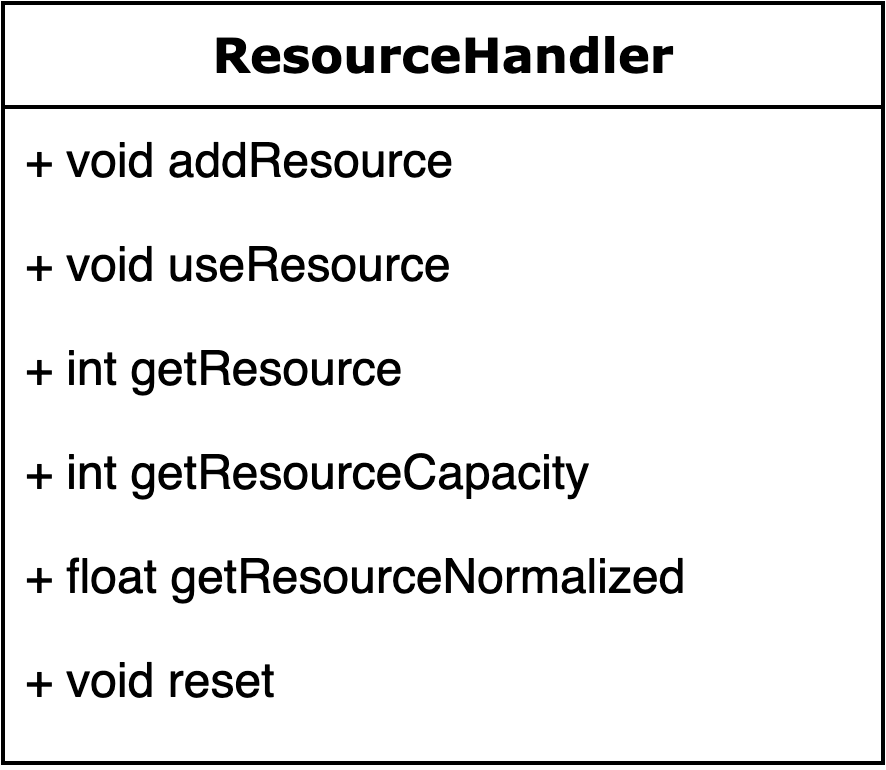
\includegraphics[scale=0.18]{images/village/architecture_diagram_resourcehandler.png}
\caption{Methoden der Klasse \inlinecode{ResourceHandler}}
\label{fig:architecture_diagram_resourcehandler}
\end{figure}

Eine Instanz des \inlinecode{ResourceHandler}s wird in der Klasse \inlinecode{Village} erzeugt und schließlich allen Agenten zugänglich gemacht. In der Funktion \inlinecode{reset} werden zunächst Obergrenzen für die Kapazitäten der einzelnen Ressourcen aufgrund der Anzahl der Agenten des Dorfes definiert. Je mehr Agenten vorhanden sind, desto höher ist die Kapazitätsgrenze, da sich die Menge der produzierten Ressourcen pro Aktion sowie die Menge der pro Agent verbrauchten Ressourcen nicht verändert. Weiterhin werden die Ressourcen zufällig initialisiert, werden aber durch Maximal- und Minimalwerte eingeschränkt. Die Funktion \inlinecode{reset} wird außerdem während des Trainings nach einer bestimmten Zeit aufgerufen, um die Ressourcen zurückzusetzen.
Die verschiedenen Typen von Ressourcen werden ebenfalls im \inlinecode{ResourceHandler} definiert. Über die Funktionen \inlinecode{addResource} und \inlinecode{useResource} können Agenten mit Ressourcen interagieren. Weiterhin besteht die Möglichkeit, in Abhängigkeit von der Kapazität einer Ressource durch die Funktion \inlinecode{getResourceNormalized} eine normalisierte Anzahl für eine Ressource zu erhalten. Der Wertebereich dieser Anzahl wird durch den Intervall $[0,1]$ definiert. Diese Normierung ist für die Observations wichtig, die idealerweise in dem genannten Intervall liegen sollten. Bei der Initialisierung der Simulation werden zufällige Werte für alle Ressourcen geliefert, die aber über einem Minimum und unter einem Maximum liegen.

\subsubsection{TimeController}
Der \inlinecode{TimeController} verwaltet das Voranschreiten der Zeit im Spiel. Der wird benötigt, um den Tagesablauf zu simulieren und die Bedürfnisse der Agenten aufgrund der vergangenen Zeit anzupassen. Abbildung \ref{fig:architecture_diagram_timecontroller} zeigt den Aufbau der Klasse.

\begin{figure}[H]
\centering
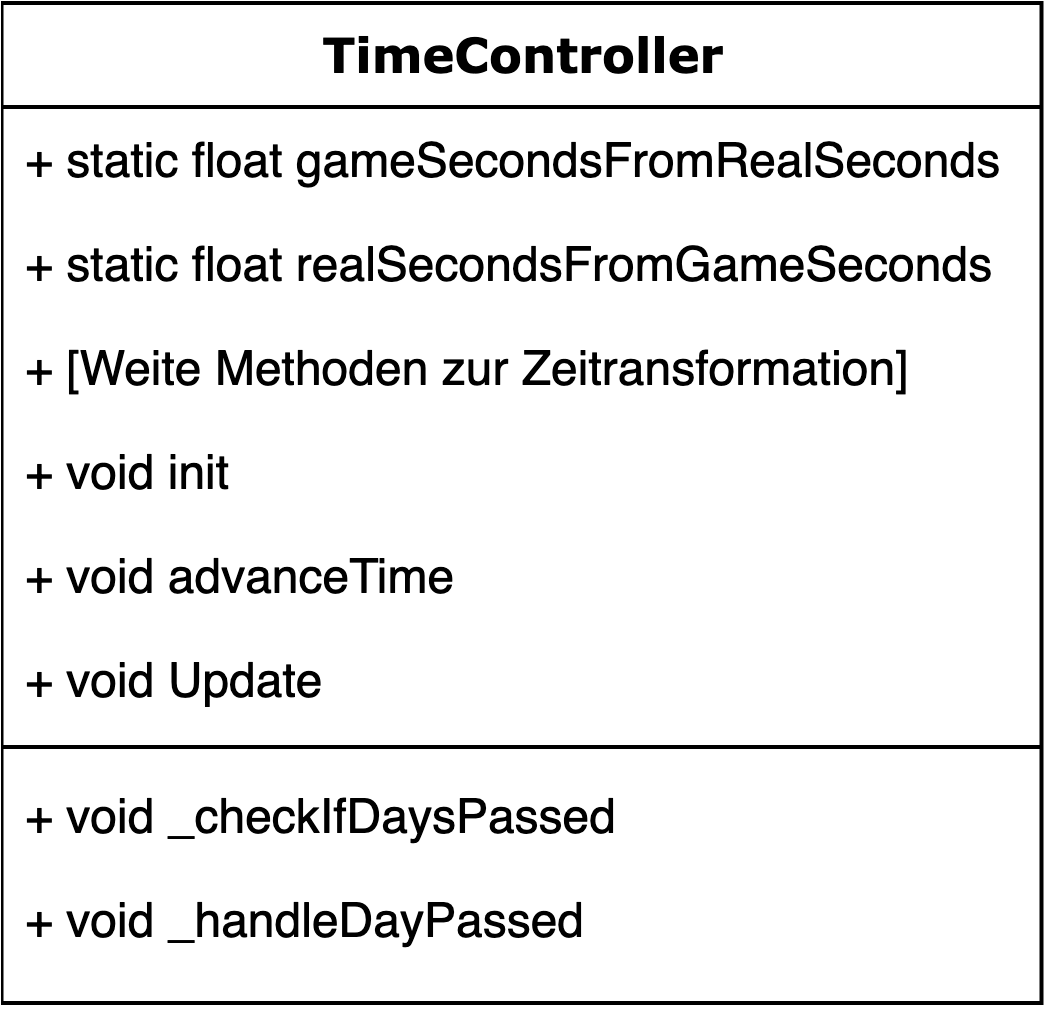
\includegraphics[scale=0.18]{images/village/architecture_diagram_timecontroller.png}
\caption{Methoden der Klasse \inlinecode{TimeController}}
\label{fig:architecture_diagram_timecontroller}
\end{figure}

Die Unityfunktion \inlinecode{Update} wird in Intervallen aufgerufen und ist dafür zuständig, alle Komponenten, die von der Zeit abhängig sind, mit der aktuellen Zeit zu versorgen. Konkret müssen der \inlinecode{LightHandler} und der \inlinecode{NpcState} jedes Agenten für jeden neuen Frame aktualisiert werden. Wie weit die Zeit voranschreitet, ist von der vergangen Zeit seit dem letzten Aufruf abhängig. Es wird in Sekunden gerechnet, da \inlinecode{Time.deltaTime} in Sekunden angegeben wird. Die Update-Funktion ruft für jeden neuen Frame die Funktion \inlinecode{advanceTime} auf:

\begin{minipage}{\linewidth}
\begin{lstlisting}[linewidth=16.4cm, label=lst:village_timecontroller_advancetime, caption=Funktion \inlinecode{advanceTime} im \inlinecode{TimeController}, xleftmargin=1cm]
public void advanceTime(float deltaTime) {
    _setCurrentTime(deltaTime);
    _village.updateTime(deltaTime, _currentTime, _daysPassed);
}
\end{lstlisting}
\end{minipage}

In der Funktion \inlinecode{\_setCurrentTime} findet anschließend die eigentliche Aktualisierung der Zeit statt:

\begin{minipage}{\linewidth}
\begin{lstlisting}[linewidth=16.4cm, label=lst:village_timecontroller_setcurrenttime, caption=Funktion \inlinecode{\_setCurrentTime} im \inlinecode{TimeController}, xleftmargin=1cm]
private void _setCurrentTime(float deltaTime) {
    _currentTime += deltaTime * ONE_SECOND_NORMALIZED * REAL_SECOND_INGAME_DURATION;
    _checkIfDaysPassed();
}
\end{lstlisting}
\end{minipage}

Wichtig ist dabei die Zeile 3. Die Konstante \inlinecode{ONE\_SECOND\_NORMALIZED} ist der auf einen ganzen Tag normierte Anteil einer Sekunde an diesem Tag:

$$ ONE\_SECOND\_NORMALIZED \;=\; \frac{1}{24 * 60 * 60} \approx 0.00012 $$

Der Wert von \inlinecode{\_currentTime} stellt die aktuelle Tageszeit dar, genormt auf einen Wert zwischen $0$ und $1$. Für jede im Spiel vergangene Sekunde wird \inlinecode{\_currentTime} also mit dem Wert $0.00012$ addiert. Im Spiel vergehen die Spiele jedoch schneller als in der Realität, weswegen \inlinecode{ONE\_SECOND\_NORMALIZED} mit \inlinecode{REAL\_SECOND\_INGAME\_DURATION} multipliziert wird.

Die Funktion \inlinecode{\_checkIfDaysPassed} prüft schließlich, ob ein Tag vergangen ist. Das ist der Fall, wenn $\_currentTime > 1f$.

\begin{minipage}{\linewidth}
\begin{lstlisting}[linewidth=16.4cm, label=lst:village_timecontroller_checkIfDaysPassed, caption=Funktion \inlinecode{\_checkIfDaysPassed} im \inlinecode{TimeController}, xleftmargin=1cm]
private void _checkIfDaysPassed() {
    _daysPassed = 0;
    while (_currentTime > 1f) {
        _days++;
        Monitor.Log("Days", _days.ToString());
        _currentTime -= 1f;
        _daysPassed += 1;
        _handleDayPassed();
    }
}
\end{lstlisting}
\end{minipage}

Die Funktion \inlinecode{advanceTime} ruft für jedes Update die Funktion \inlinecode{Village.updateTime} auf. Darin wird die neue Zeit an alle weiteren Komponenten weitergeleitet, die diese benötigen. Konkret sind das alle mit dem Dorf verbundenen Agenten mit ihren Bedürfnissen sowie der \inlinecode{LightHandler}:

\begin{minipage}{\linewidth}
\begin{lstlisting}[linewidth=16.4cm, label=lst:village_timecontroller_updatetime, caption=Funktion \inlinecode{updateTime} im \inlinecode{TimeController}, xleftmargin=1cm]
public void updateTime(float deltaTime, float currentTime, int daysPassed) {
    foreach (NpcAgent npc in _villageNpcs) {
        npc.updateNpc(deltaTime, currentTime, daysPassed);
    }
    _lightHandler.updateLights(currentTime);
}
\end{lstlisting}
\end{minipage}

Weiterhin bietet der \inlinecode{TimeController} durch die Funktionen \inlinecode{gameSecondsFromRealSeconds} und \inlinecode{realSecondsFromGameSeconds} sowie weiteren Methoden eine Schnittstelle für die Umrechnung zwischen Echtzeit und Spielzeit. In einer Konstante wird dafür die Dauer einer reellen Sekunde für spätere Berechnungen gespeichert. Zusätzlich wird ein normalisierter Wert für den Anteil einer Sekunde an einem Tag festgelegt:

\begin{minipage}{\linewidth}
\begin{lstlisting}[linewidth=16.4cm, label=lst:village_timecontroller_seconds_constants, caption=Berechnung der Dauer einer Sekunde in Simulationszeit, xleftmargin=1cm]
public const float REAL_SECOND_INGAME_DURATION = SECONDS_PER_DAY / DAY_CYCLE_REAL_SECONDS;
public const float ONE_SECOND_NORMALIZED = 1f / SECONDS_PER_DAY;
\end{lstlisting}
\end{minipage}

\inlinecode{SECONDS\_PER\_DAY} beträgt logischerweise $ 60 * 60 * 24 Sekunden $. Mithilfe dieser Werte kann die Realzeit nun in Simulationszeit umgerechnet werden:

\begin{minipage}{\linewidth}
\begin{lstlisting}[linewidth=16.4cm, label=lst:village_timecontroller_time_calculation, caption=Umrechnung von Simulationszeit und Realzeit, xleftmargin=1cm]
public static float realSecondsFromGameSeconds(float gameSeconds) {
    return gameSeconds / REAL_SECOND_INGAME_DURATION;
}

public static float gameSecondsFromRealSeconds(float realSeconds) {
    return ONE_SECOND_NORMALIZED * DAY_CYCLE_REAL_SECONDS * realSeconds;
}
\end{lstlisting}
\end{minipage}



\subsection{LightHandler}
Der \inlinecode{LightHandler} ist dafür zuständig, Tageszeiten zu simulieren, indem der Sonnenstand geregelt und Lichtquellen kontrolliert werden. In der Abbildung \ref{fig:architecture_diagram_lighthandler} wird der Aufbau der Klasse anhand ihrer Funktion verdeutlicht. 
Im \inlinecode{LightHandler} werden zusätzlich folgende Felder definiert:

\begin{itemize}
    \item \inlinecode{List<Light> \_agentLights}: Alle Lampen der Agenten. Jeder \ac{npc} verfügt über eine Lichtquelle, die sie an ihrem Körper tragen.
    \item \inlinecode{List<Light> \_villageLamps}: Alle Laternen, die im und um das Dorf herum positioniert wurden.
    \item \inlinecode{List<Light> \_bonfires}: Alle Lagerfeuer in der Simulation.
    \item \inlinecode{List<Transform> \_bonfireParticleTransforms}: Die Partikeleffekte der Lagerfeuer.
    \item \inlinecode{Light \_sun}: Eine Lichtquelle, die die Sonne simuliert.
\end{itemize}

\begin{figure}[H]
\centering
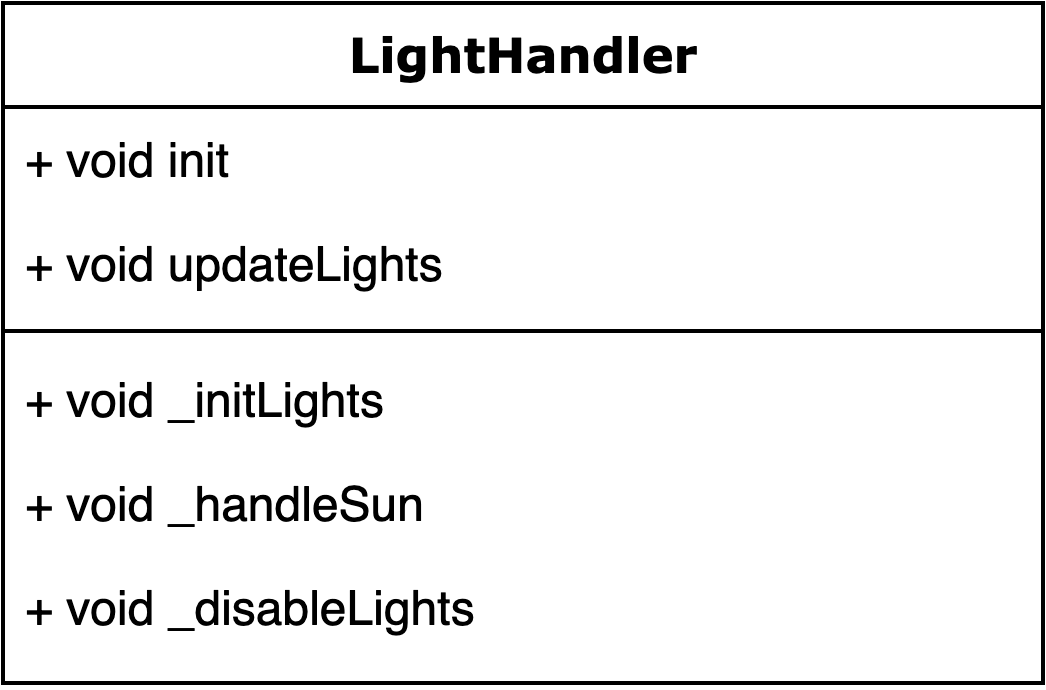
\includegraphics[scale=0.18]{images/village/architecture_diagram_lighthandler.png}
\caption{Methoden der Klasse \inlinecode{LightHandler}}
\label{fig:architecture_diagram_lighthandler}
\end{figure}

Die Funktion \inlinecode{\_initLights} sucht nach allen in der Szene enthaltenen Lichtquellen vom Typ \inlinecode{Light} und speichert diese. \inlinecode{Light} ist der Standardtyp für Lichtquellen in Unity. \inlinecode{Light} ist eine Komponente, die an ein \inlinecode{GameObject} angefügt wird.
Innerhalb der Funktion \inlinecode{updateLights} werden bestimmte Parameter der Lichtquellen in Abhängigkeit von der aktuellen Zeit verändert. Die Lichtquellen der Agenten sowie die Laternen im Dorf werden, zu einer bestimmten Uhrzeit an- und zu einer bestimmten Uhrzeit wieder ausgeschaltet. Nachts leuchten diese Lichtquellen also durchgehend. Weiterhin gibt es in der Stadt eine Menge von Lagerfeuern. Tagsüber glühen diese leicht, mit zunehmender Dunkelheit erhöht sich ihre Intensität. Die Partikeleffekte werden dann zusätzlich leicht nach oben verschoben, sodass sie weiter aus dem Boden herausragen und es so wirkt, als würde das Feuer stärker brennen. Jeder einzelne Partikel des Lagerfeuers stellt eine kleine Lichtquelle dar, um einen realistischen Feuereffekt zu simulieren.
Weiterhin wird in der Funktion \inlinecode{\_handleSun} sowohl die Intensität als auch die Position und Ausrichtung der Sonne in Abhängigkeit von der Zeit angepasst, wie in \ref{lst:lighthandler_sun} zu sehen.

\begin{minipage}{\linewidth}
\begin{lstlisting}[linewidth=16.4cm, label=lst:lighthandler_sun, caption=Anpassung der Sonne durch den \inlinecode{LightHandler}, xleftmargin=1cm]
private void _handleSun(float currentTime) {
    _sun.transform.localRotation = Quaternion.Euler((currentTime * 360f) - 90f, 170f, 0f);

    float multiplier = 1f;
    if (currentTime <= 0.28f) {
        multiplier = Mathf.Clamp01((currentTime - 0.25f) * (1f / 0.03f));
    }
    else if (currentTime >= 0.75f) {
        multiplier = Mathf.Clamp01(1f - ((currentTime - 0.78f) * (1f / 0.03f)));
    }
    _sun.intensity = multiplier * 1.5f;
}
\end{lstlisting}
\end{minipage}

Damit die Sonne sich wie eine Sonne verhält, muss die entsprechende Lichtquelle in den Lichteinstellungen der Unity-Szene als \Fachbegriff{Sun} markiert werden. Sie erhält dann automatisch das Aussehen einer Sonne und wird entsprechend positioniert. Unity übernimmt dann die eigentliche Beleuchtung und passt das \inlinecode{Light} so an, dass es eine überzeugende Sonne darstellt. Weiterhin verändert die Position der Sonne nun die Farbgebung der verwendeten Skybox - sobald die Sonne sich an den Rand des Horizonts bewegt, wird ein Sonnenuntergang bzw. Sonnenaufgang dargestellt. Wenn sie sich unter dem Horizont befindet, wird eine andere Textur für die Skybox verwendet, die in diesem Fall einen dunklen Sternenhimmel zeigt. Nun muss nur noch die Rotation der Sonne angepasst werden. Dadurch beschreibt die Position der Sonne im Verlauf des Tages eine Kreisbahn um das Dorf herum. Weiterhin wird die Intensität angepasst, sodass die Lichtverhältnisse mit der Tageszeit übereinstimmen. In den Abbildungen \ref{fig:village_village_night_1} und \ref{fig:village_village_night_2} ist beispielhaft zu erkennen, wie die Stadt nachts beleuchtet wird. Zum Vergleich wurden hier die selben Motive und Kameraeinstellungen verwendet, wie bereits in den Grafiken \ref{fig:village_village_day_1} und \ref{fig:village_village_day_2}.

\begin{figure}[H]
\centering
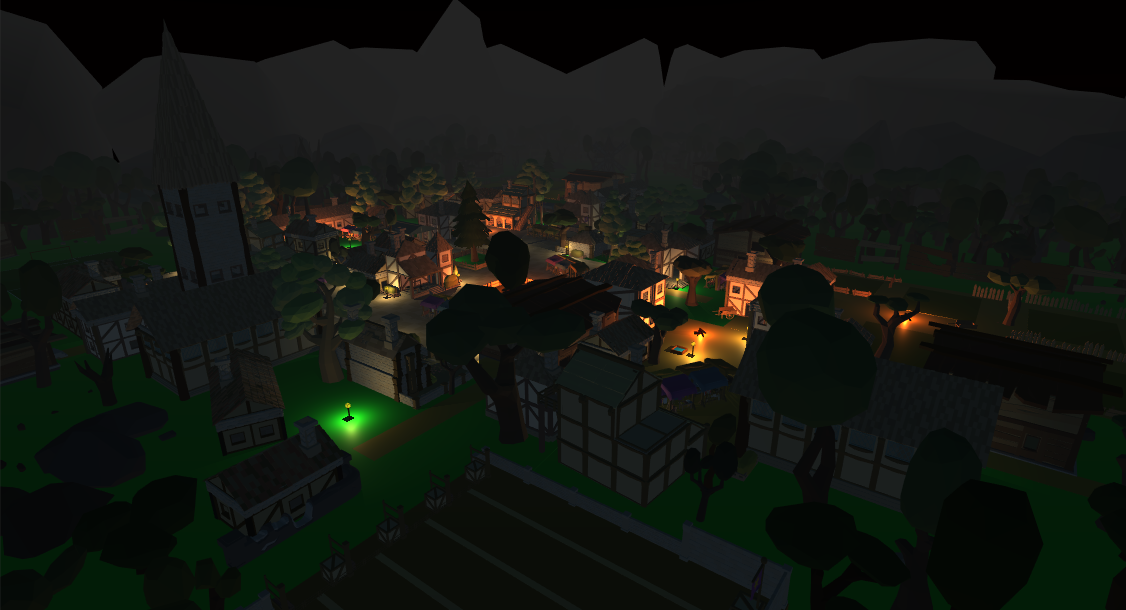
\includegraphics[scale=0.55]{images/village/village_village_night_1.PNG}
\caption{Modellierte Stadt, äußere Ansicht, nächtliche Beleuchtung}
\label{fig:village_village_night_1}
\end{figure}

\begin{figure}[H]
\centering
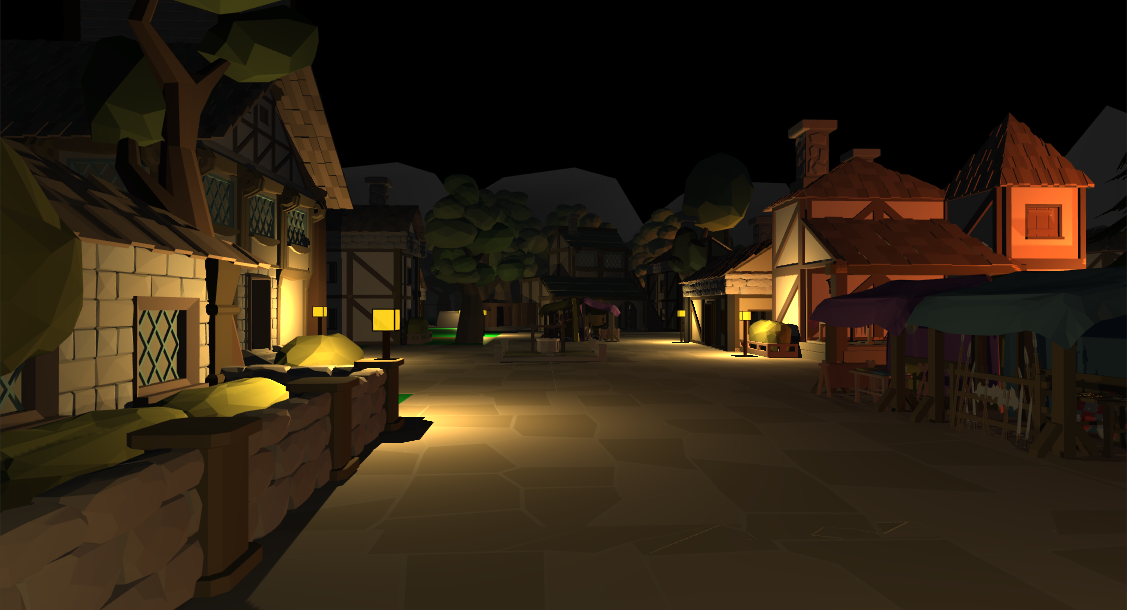
\includegraphics[scale=0.55]{images/village/village_village_night_2.png}
\caption{Modellierte Stadt, innere Ansicht, nächtliche Beleuchtung}
\label{fig:village_village_night_2}
\end{figure}


Für das Training des Agenten ist die Performance der Anwendung ausschlaggebend. Da die Entscheidungsfindung der Agenten in keiner Weise von der Beleuchtung der Szene abhängt, jedoch einen großen Teil der aufgewendeten Leistung in einer Simulation beansprucht, werden alle Lichtquellen während des Trainings automatisch deaktiviert. Dafür wird \inlinecode{GameAcademy.IS\_TRAINING} geprüft. In diesem Fall wird der \inlinecode{Lighthandler} nur initialisiert und dann deaktiviert, da keine Lichtquellen mehr zeitabhängig angepasst werden müssen.







\subsection{Implementierung des Agenten und dessen Subkomponenten}
Insgesamt wurden 16 Observations und 29 diskrete Aktionen verwendet, die dem Agenten zur Auswahl stehen. Es werden ausschließlich On Demand Decisions verwendet (siehe Kapitel \ref{ml_unity}). Der Agent wird während des Trainings nach einer festgelegten Anzahl von Entscheidungen zurückgesetzt. Das Training erfolgt mit dem \ac{ppo}-Algorithmus (siehe Abschnitt \ref{proximal_policy_optimization}) und verwendet ein neuronales Netz mit mehreren Schichten und mehreren hundert Neuronen. Es können beliebig viele Agenten verwendet werden. Zunächst werden die grundsätzlichen Funktionen der Klasse \inlinecode{NpcAgent} betrachtet, welche für die Realisierung der Agenten erstellt wurde.
Die Funktionen der Klasse werden in der Abbildung \ref{fig:architecture_diagram_agent} dargestellt.

\begin{figure}[H]
\centering
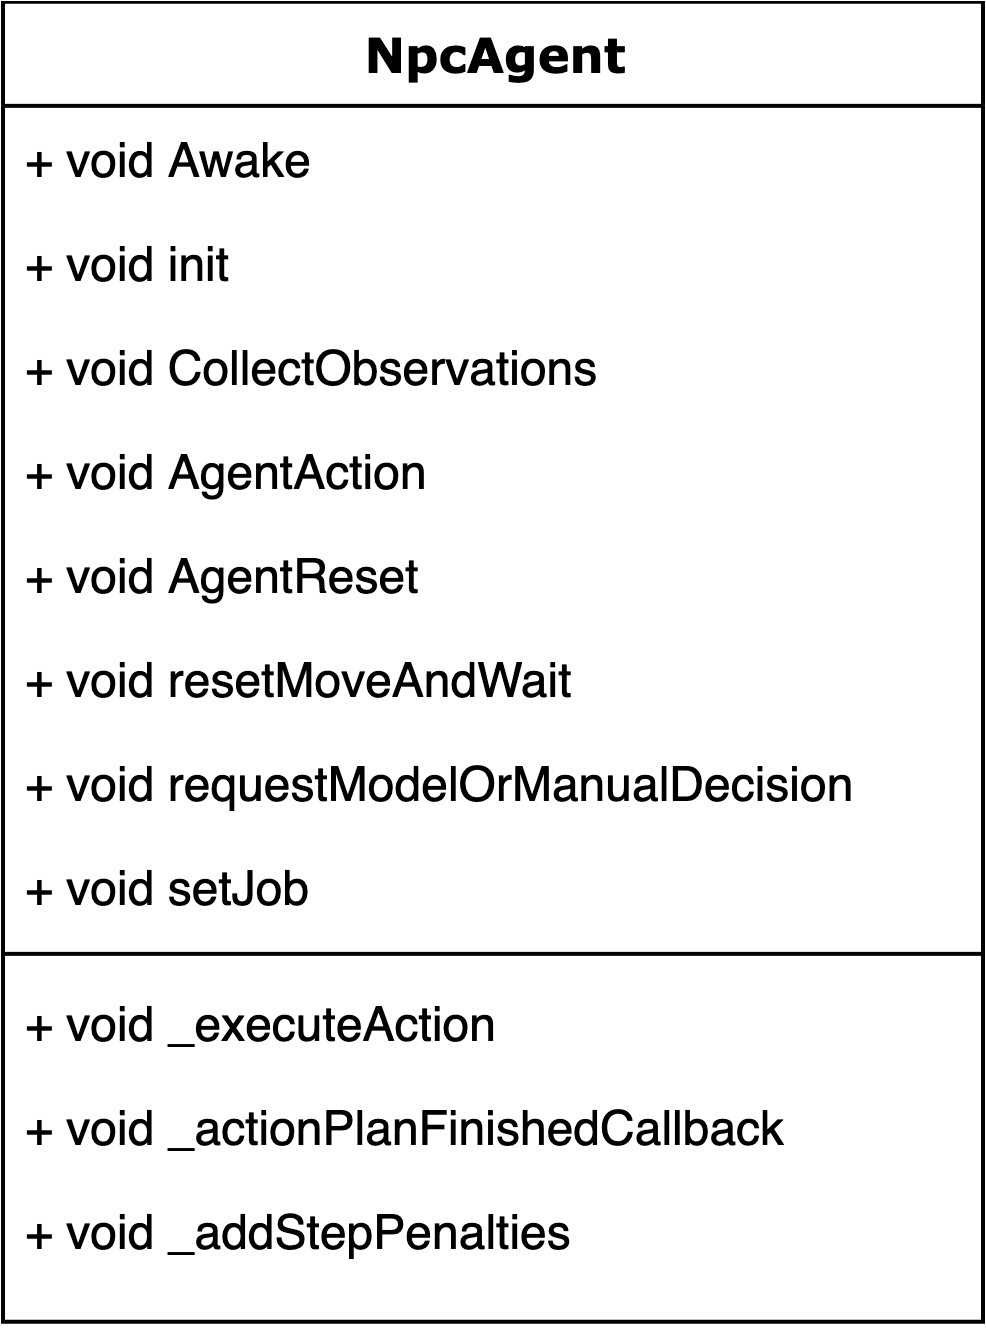
\includegraphics[scale=0.18]{images/village/architecture_diagram_agent.png}
\caption{Methoden der Klasse \inlinecode{NpcAgent}}
\label{fig:architecture_diagram_agent}
\end{figure}

Der \inlinecode{NpcAgent} verwendet sogenannte \Fachbegriff{ActionPlans} für die sequentielle Ausführung von Aktionen. Diese werden im späteren Abschnitt \ref{action_plans} behandelt.

Die Funktionen \inlinecode{CollectObservations}, \inlinecode{AgentAction}, \inlinecode{AgentReset} und \inlinecode{Awake} sind bereits bekannt (siehe Kapitel \ref{ml_unity}).
Die Funktionen \inlinecode{Awake} \inlinecode{setJob} und \inlinecode{init} werden benötigt, um den Agenten zu intitialisieren. Weiterhin werden \inlinecode{resetMoveAndWait} und \inlinecode{AgentReset} verwendet, um den Agenten beispielsweise nach dem Abschließen einer Episode zurückzusetzen. In der Funktion \inlinecode{\_actionPlanFinishedCallback} wird nach dem Ausführen einer Aktion geprüft, ob eine Episode abgeschlossen ist oder eine neue Entscheidung mit \inlinecode{requestModelOrManualDecision} angefragt werden soll. In der Funktion \inlinecode{\_addStepPenalties} werden darüber hinaus Bestrafungen ausgeschüttet. Konkret wird für jedes Bedürfnis des Agenten, das unter einer bestimmten Grenze liegt, eine Bestrafung zugewiesen.

Der Beobachtungsraum des Agenten wird durch die in der Funktion \inlinecode{CollectObservations} getätigten Observations beschrieben, wie in Listing \ref{lst:village_agent_observations} zu sehen:

\begin{minipage}{\linewidth}
\begin{lstlisting}[linewidth=16.4cm, label=lst:village_agent_observations, caption=Beobachtungen des Agenten, xleftmargin=1cm]
public override void CollectObservations() {
    AddVectorObs(_npcState.NeedHunger);
    AddVectorObs(_npcState.NeedThirst);
    AddVectorObs(_npcState.NeedEducation);
    AddVectorObs(_npcState.NeedCommunication);
    AddVectorObs(_npcState.NeedFaith);
    AddVectorObs(_npcState.Recreation);
    AddVectorObs(_npcState.Exhaustion);
    AddVectorObs(_npcState.AttFittness);
    AddVectorObs(_npcState.AttIntelligence);
    AddVectorObs(_npcState.AttCompanionship);
    AddVectorObs(_npcState.AttCommodities);
    AddVectorObs(_npcState.AttFerocity);
    AddVectorObs(_npcState.Sleep);
    AddVectorObs(_npcState.Work);
    AddVectorObs(_npcState.getMoneyNormalized());
    AddVectorObs(_currentTime);

    SetActionMask(_actionMaskingHandler.getIntActionMask(this));
}
\end{lstlisting}
\end{minipage}

Als Input für das neuronale Netz werden also sämtliche Bedürfnisse sowie die Attribute, die Menge des Geldes des Agenten und die aktuelle Zeit verwendet. Insgesamt kommen so 16 Observations zustande.
Der Handlungsraum besteht aus 29 möglichen Aktionen für die Befriedigung von Bedürfnissen. Die Funktion \inlinecode{AgentAction} ist in Listing \ref{lst:agent_agentaction} zu erkennen:

\begin{minipage}{\linewidth}
\begin{lstlisting}[linewidth=16.4cm, label=lst:agent_agentaction, caption=Funktion \inlinecode{AgentAction} des Agenten, xleftmargin=1cm]
public override void AgentAction(float[] vectorAction, string textAction) {
    _executeAction(NpcActions.actionNameFromId(Mathf.RoundToInt(vectorAction[0])));
}

private void _executeAction(string actionId) {
    [...] // Logging etc.
    _action = actionId;
    _academy.IncrementNumAgentActions();
    _numActions++;
    _actionHandler.runActionPlan(actionId);
}
\end{lstlisting}
\end{minipage}

Zunächst wird aus dem Float-Wert, der von ML-Agents geliefert wird, ein Integer gemacht. Das ist sinnvoll, weil hier diskrete Entscheidungen verwendet werden, die durch einen Integer-Wert referenziert werden. In der Funktion \inlinecode{\_executeAction} werden schließlich nach einigen Logging-Anweisungen Zähler inkrementiert und durch die Anweisung \inlinecode{\_actionHandler.runActionPlan} der \inlinecode{ActionHandler} aufgerufen, der dem Identifier der Aktion einen ausführbaren ActionPlan zuweist. Im nächsten Abschnitt wird dieses Vorgehen erläutert. Es wird darauf eingegangen, wie die Aktionen des Agenten beschrieben und ausgeführt werden können.


\subsubsection{ActionPlans}\label{action_plans}
Für die Ausführung von Aktionen wurde eine eigene Kontroll- und Datenstruktur entwickelt, die eine Reihe von untergeordneten Aktionen enthält. Die Struktur ist allgemein für sequentielle Ausführungen von Aufgaben nutzbar, deren zeitliche Dauer zum Zeitpunkt der Ausführung unbekannt sein kann. In dieser Arbeit wurden diese \Fachbegriff{ActionPlans} genannten Konstrukte für die Ausführung der Aktionen des Agenten angefertigt. Im Folgenden werden sie näher erläutert.
ActionPlans erben von der Basisklasse \inlinecode{BaseActionPlan}. Die Abbildung \ref{fig:architecture_diagram_baseactionplan} zeigt die Funktionen der Klasse:

\begin{figure}[H]
\centering
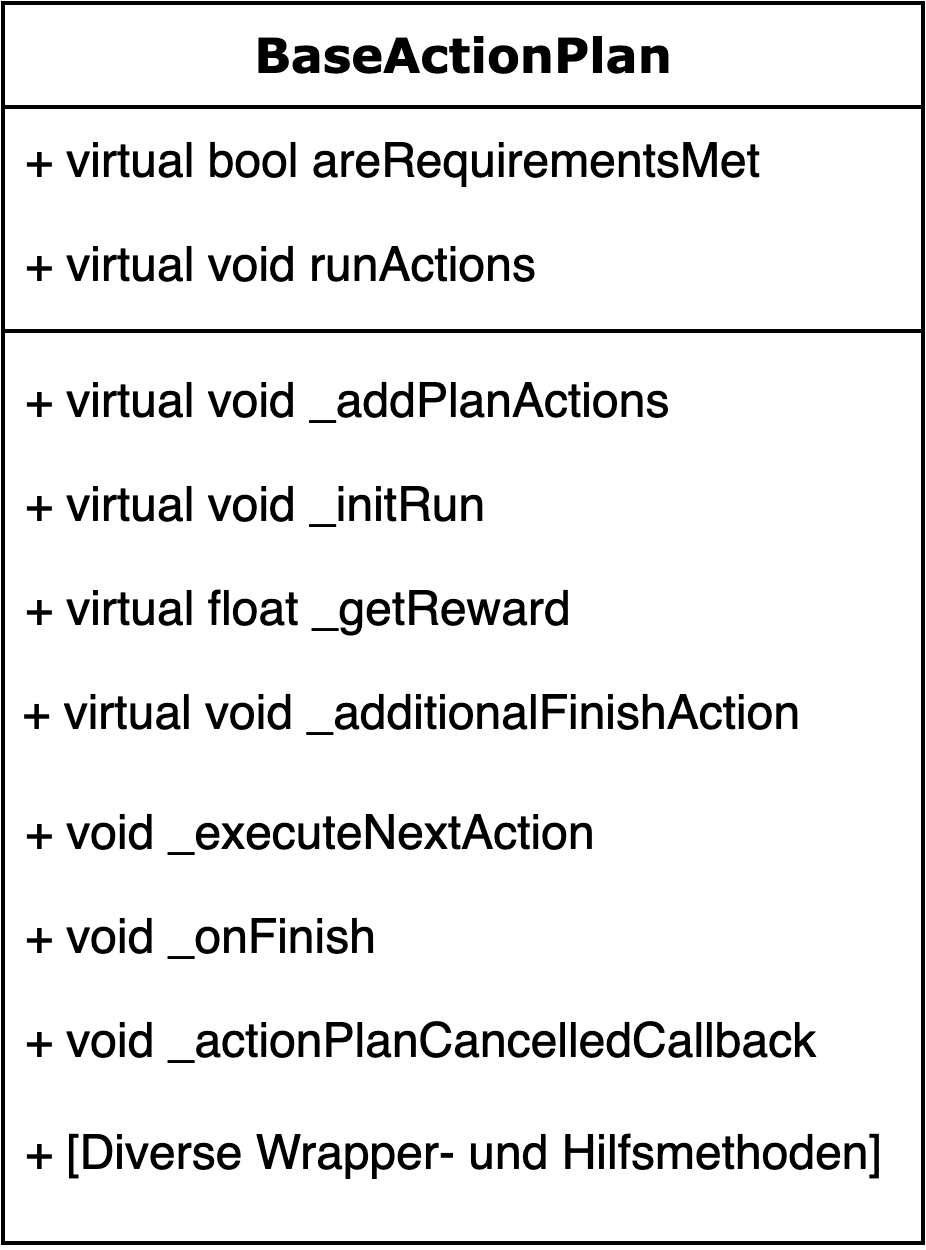
\includegraphics[scale=0.18]{images/village/architecture_diagram_baseactionplan.png}
\caption{Methoden der Klasse \inlinecode{BaseActionPlan}}
\label{fig:architecture_diagram_baseactionplan}
\end{figure}

In der Klasse \inlinecode{NpcActions} werden String-Identifier für alle Aktionen definiert, zum Beispiel \inlinecode{NpcActions.HUNGER\_BREAD}. \inlinecode{NpcActions} liefert weiterhin ein Mapping dieser Identifier zu den numerischen Identifiern von Aktionen, die ML-Agents beim Aufruf der Funktion \inlinecode{AgentAction} liefert. Anhand dieser Identifier wird jeder Aktion aus dem Aktionsraum des neuronale Netzes genau ein übergeordneter ActionPlan zugewiesen. 
Die Menge aller Sub-Aktionen eines ActionPlans beschreibt genau eine übergeordnete Aktion. Von der Basisklasse \inlinecode{BaseActionPlan} müssen bestimmte Funktionen überschrieben werden. Innerhalb der Funktion \inlinecode{\_addPlanActions} werden eine Reihe von Aktionen definiert, die sequentiell ausgeführt werden, wie beispielsweise das Navigieren des Agenten zu einer Zielposition. Zusätzlich zur Ausführung von Aktionen werden hier Effekte und Voraussetzungen für Aktionen verwaltet. Die Ausführung der einzelnen Teilaktionen erfolgt in der Funktion \inlinecode{nextActionExecutedCallback}. Nach der Ausführung jeder Einzelaktion wird ein Callback aufgerufen, wie in Listing \ref{lst:village_actionplan_single_action_callback} zu erkennen. Es handelt sich um eine einfache Funktion ohne Parameter, die jeder Einzelaktion im Konstruktor mitgegeben wird.

\begin{minipage}{\linewidth}
\begin{lstlisting}[linewidth=16.4cm, label=lst:village_actionplan_single_action_callback, caption=ActionPlan-Callback, xleftmargin=1cm]
private void nextActionExecutedCallback()
{
    _currentAction += 1;

    if (_currentAction >= _actions.Count) {
        _onFinish();
        _allActionsExecutedCallback();
    } else {
        _executeNextAction();
    }
}
\end{lstlisting}
\end{minipage}

Wenn weitere Aktionen vorhanden sind, wird die nächste Aktion aus der Liste ausgeführt. Auf die Terminierung der letzten Aktion folgt der Aufruf eines weiteren, übergeordneten Callbacks \inlinecode{\_allActionsExecutedCallback}. Auch hier handelt es sich um eine einfache parameterlose Funktion. Der Callback ruft im \inlinecode{NpcAgent} die Funktion \inlinecode{\_actionPlanFinishedCallback} auf und führt zu einer Anfrage an das ML-Agents Toolkit für eine neue Entscheidung. Nach der Ausführung der Aktionen wird weiterhin eine Belohnung oder eine Bestrafung für den Agenten ausgeschüttet, indem \inlinecode{\_onFinish} aufgerufen wird. Zusätzlich können abschließend beispielsweise Ressourcen hinzugefügt werden, die die Aktion produziert hat.

Zum Start des ActionPlans wird die in Listing \ref{lst:village_actionplan_runactions} dargestellte Funktion \inlinecode{runActions} verwendet:

\begin{minipage}{\linewidth}
\begin{lstlisting}[linewidth=16.4cm, label=lst:village_actionplan_runactions, caption=Starten eines ActionPlans, xleftmargin=1cm]
public void runActions() {
    _npc.VillageInfo.changeAmountForAction(true, _actionType);
    _currentAction = 0;
    _initRun();

    if (_actions == null || _actions.Count == 0) {
        _onFinish();
        _allActionsExecutedCallback();
    } else {
        _executeNextAction();
    }
}
\end{lstlisting}
\end{minipage}

Im Konstruktor von \inlinecode{BaseActionPlan} wird die abstrakte Funktion \inlinecode{\_addPlanActions} definiert, welche von Unterklassen überschrieben werden muss. Darin müssen die Aktionen des ActionPlans hinzugefügt werden, indem sie durch \inlinecode{\_actions.Add(newAction)} in eine \inlinecode{List<BaseAction>} geschrieben werden. In \inlinecode{runActions} wird zunächst die erste dieser Aktionen mit dem Index $\_currentAction = 0$ ausgeführt. Nach jeder ausgeführten Aktion wird der Index erhöht und die nächste Funktion ausgeführt.

Ein Beispiel für eine Implementierung eines vollständigen ActionPlans ist in \ref{lst:village_butcher-actionplan} zu finden. Der ActionPlan \inlinecode{ReligionChurchActionPlan} beschreibt den Vorgang eines Agenten, die Kirche zu besuchen, um sein Bedürfnis nach \Fachbegriff{Glauben} aufzufüllen.

\begin{minipage}{\linewidth}
\begin{lstlisting}[linewidth=16.4cm, label=lst:village_butcher-actionplan, caption=Beispielhafter ActionPlan \inlinecode{ReligionChurchActionPlan}, xleftmargin=1cm, basicstyle=\footnotesize]
public class ReligionChurchActionPlan : BaseActionPlan
{
    public ReligionChurchActionPlan(Action allActionsExecutedCallback,
                                   NpcAgent npc)
        : base(NpcActions.RELIGION_CHURCH, allActionsExecutedCallback, npc) { }

    public override bool areRequirementsMet() {
        if (!_hasFreeSpot(LocationTypes.CHURCH)) return false;
        return true;
    }

    protected override float _getReward() {
        return _getNeedReward(NpcState.NEED_FAITH, NEED_REWARD_MULTIPLIER);
    }

    protected override void _addPlanActions() {
        _addMoveAction(LocationTypes.CHURCH);
        _addWaitAction(DEFAULT_ACTION_SECONDS);
        _addVacateAction(LocationTypes.CHURCH);
    }

    protected override void _additionalFinishAction() {
        _npcState.satisfyNeedByType(NpcState.NEED_FAITH, DEFAULT_NEED_GAIN);
    }
}
\end{lstlisting}
\end{minipage}

Bevor die Entscheidung getroffen wird, welcher ActionPlan ausgeführt werden soll, wird die Funktion \inlinecode{areRequirementsMet} jedes ActionPlans aufgerufen. Diese prüft einige Bedingungen, die erfüllt sein müssen, damit der ActionPlan ausgeführt werden darf. Die Voraussetzung für die Ausführung in dem obigen Beispiel stellt die Bedingung auf, dass mindestens ein freier Slot in einem Gebäude des Typs \inlinecode{CHURCH} vorhanden sein muss.
Die einzelnen Teilaktionen des ActionPlans werden in \inlinecode{\_addPlanActions} definiert. Zunächst wird eine \inlinecode{MoveAction} definiert, die den Agenten zur Kirche bewegt. Diese Aktion beinhaltet die Reservierung eines Slots für den Agenten. Weiterhin wird eine \inlinecode{WaitAction} definiert, welche typischerweise genutzt wird, um die Ausführung einer beliebigen Tätigkeit zu simulieren. Effektiv bleibt der Agent an einem Ort stehen und wartet, bis eine gewisse Zeit abgelaufen ist. Anschließend wird eine \inlinecode{VacateAction} ausgeführt, welche dafür sorgt, dass zum Ende des Ausführungsprozesses des ActionPlans der reservierte Slot für den Agenten wieder freigegeben wird.
Nach der Ausführung der Aktionen wird schließlich durch die Funktion \inlinecode{\_getReward} die Belohnung definiert. Diese hängt von dem initialen Bedürfnis nach Glauben ab, das zu Beginn der Ausführung des ActionPlans festgestellt wurde. Der Vorgang wird im \inlinecode{BaseActionPlan}, unter anderem in der Funktion \inlinecode{\_initRun}, beschrieben. Als letztes wird das Bedürfnis des Agenten nach Glauben aufgefüllt.

Alle ActionPlans eines Agenten werden im \inlinecode{ActionHandler} erzeugt. Mithilfe des in \inlinecode{NpcActions} definierten Mappings werden die ActionPlans in einem \inlinecode{Dictionary<String,BaseActionPlan>} hinterlegt. Sobald eine neue Aktion des Agenten mit \inlinecode{AgentAction} gestartet wird, wählt der \inlinecode{ActionHandler} den zum Identifier der Aktion passenden ActionPlan aus.

In der Abbildung \ref{fig:architecture_diagram_actionhandler} ist der Aufbau der Klasse \inlinecode{ActionHandler} zu erkennen:

\begin{figure}[H]
\centering
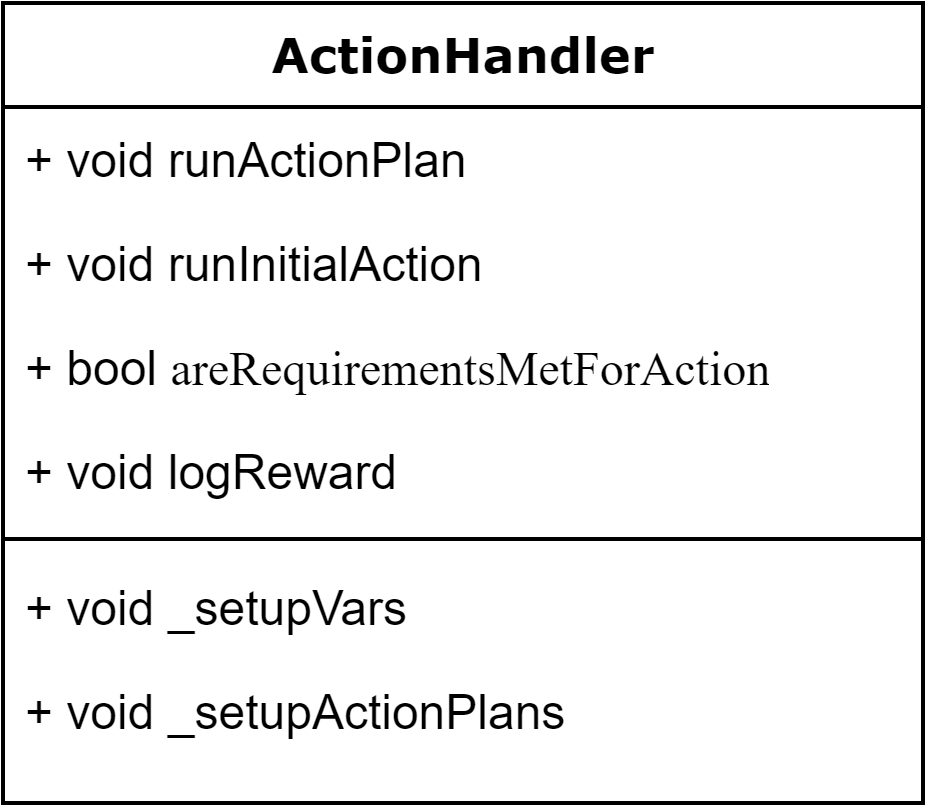
\includegraphics[scale=0.18]{images/village/architecture_diagram_actionhandler.png}
\caption{Methoden der Klasse \inlinecode{ActionHandler}}
\label{fig:architecture_diagram_actionhandler}
\end{figure}

Die Funktion \inlinecode{runInitialAction} wird verwendet, um nach der Initialisierung des Dorfes für jeden Agenten eine \inlinecode{WaitAction} mit zufälliger Dauer durchzuführen, sodass nicht alle Agenten zur selben Zeit anfangen, Aktionen auszuführen. Damit wird vermieden, dass Engpässe bezüglich der Kapazität bestimmter Gebäude entstehen.
Die Funktion \inlinecode{areRequirementsMetForAction} dient lediglich als Wrapper für die \inlinecode{areRequirementsMet}-Funktionen der einzelnen ActionPlans und wird vom \inlinecode{ActionMaskingHandler} aufgerufen.


\paragraph{Belohnungen}
Die Belohnungen der Aktionen des Agenten werden ebenfalls in den ActionPlans definiert. Dafür wurde eine Reihe von Hilfsfunktionen erstellt, zum Beispiel \inlinecode{\_getNeedReward} oder \inlinecode{\_getRecreationReward}. Die Zusammensetzung der Belohnungen kann in den jeweiligen ActionPlans im Programmcode betrachtet werden.


\paragraph{Teilaktionen des ActionPlans}
Zusätzlich zu den genannten Methoden werden diverse weitere Wrapper- und Hilfsmethoden implementiert, wie beispielsweise die Funktion \inlinecode{\_moveAndWaitRealSeconds}, die automatisch die Teilaktionen \inlinecode{MoveAction}, \inlinecode{VacateAction} und \inlinecode{WaitAction} hinzufügt, um zu einem Ort zu navigieren und dort zu verweilen. Diese Teilaktionen des ActionPlans erben von der Klasse \inlinecode{BaseAction}. Die Implementierung dieser Basisklasse ist im folgenden Listing zu erkennen:

\begin{minipage}{\linewidth}
\begin{lstlisting}[linewidth=16.4cm, label=lst:implementation_baseaction, caption=Implementierung von \inlinecode{BaseAction}, xleftmargin=1cm, basicstyle=\footnotesize]
public class BaseAction {
    protected string _actionType;
    protected NpcAgent _npc;
    protected TimeController _timeController;

    public BaseAction(string actionType, NpcAgent npc) {
        _actionType = actionType;
        _npc = npc;
        _timeController = GameObject.FindObjectOfType<TimeController>();
    }

    public virtual IEnumerator execute(Action callback,
                                       Action cancelCallback) {
        throw new System.NotImplementedException("Function execute not implemented for " + this.GetType());
    }
}
\end{lstlisting}
\end{minipage}

Klassen, die von \inlinecode{BaseAction} erben, müssen nur die \inlinecode{execute}-Funktion überschreiben und eine Callbackfunktion aufrufen, sobald die Teilaktion abgeschlossen wurde.

Um den Agenten zu einem Zielort zu bewegen wird die \inlinecode{MoveAction} verwendet. Diese interagiert zunächst mit dem \inlinecode{LocationHandler}, um einen Zielort zu erlangen und schließlich mit dem \inlinecode{MoveHandler}, um den Agenten zum Ziel zu navigieren. In der Abbildung \ref{fig:architecture_diagram_movehandler} wird der Aufbau der Klasse \inlinecode{MoveHandler} verdeutlicht:

\begin{figure}[H]
\centering
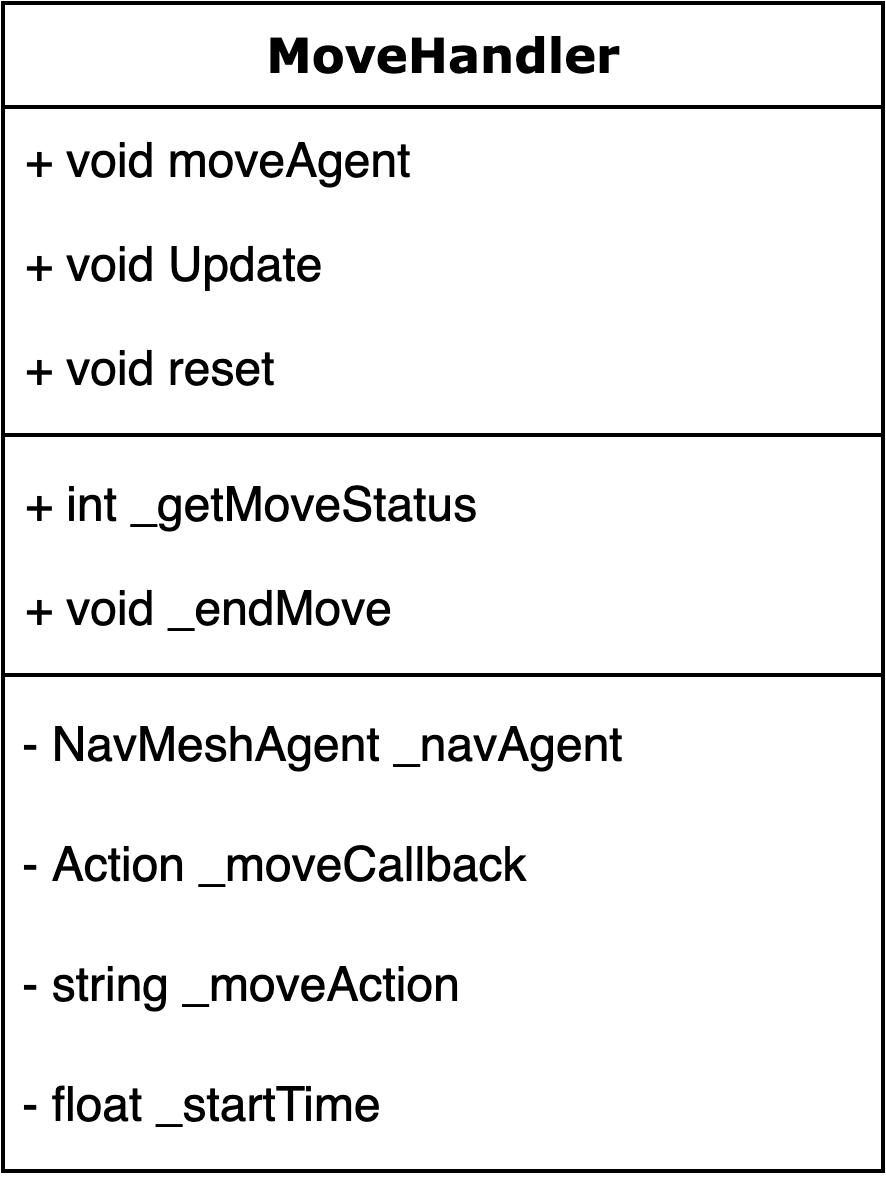
\includegraphics[scale=0.18]{images/village/architecture_diagram_movehandler.png}
\caption{Methoden der Klasse \inlinecode{MoveHandler}}
\label{fig:architecture_diagram_movehandler}
\end{figure}

Die Funktion \inlinecode{moveAgent} startet die Navigation zum Ziel. Das Feld \inlinecode{\_navAgent} referenziert den \inlinecode{NavMeshAgent}, der verwendet wird, um auf dem NavMesh zu navigieren (siehe Abschnitt \ref{agent_navigation}). Durch die Anweisung \inlinecode{\_navAgent.SetDestination(destination)} wird die Navigation des Agenten zu seinem Zielort gestartet. Zu Logging-Zwecken wird außerdem die Startzeit der Aktion im Feld \inlinecode{\_startTime} gespeichert. Die \inlinecode{Update}-Funktion prüft anschließend mit jedem neuen Frame den Status des Agenten mithilfe der Funktion \inlinecode{\_getMoveStatus}. Sobald diese Funktion den Status \inlinecode{MOVE\_STATUS\_STOPPED} zurückgibt, hat der Agent sein Ziel erreicht und ein Callback wird aufgerufen, um zurück zur \inlinecode{MoveAction} zu springen, welche wiederum einen weiteren Callback zum jeweiligen ActionPlan ausführt.

\begin{figure}[H]
\centering
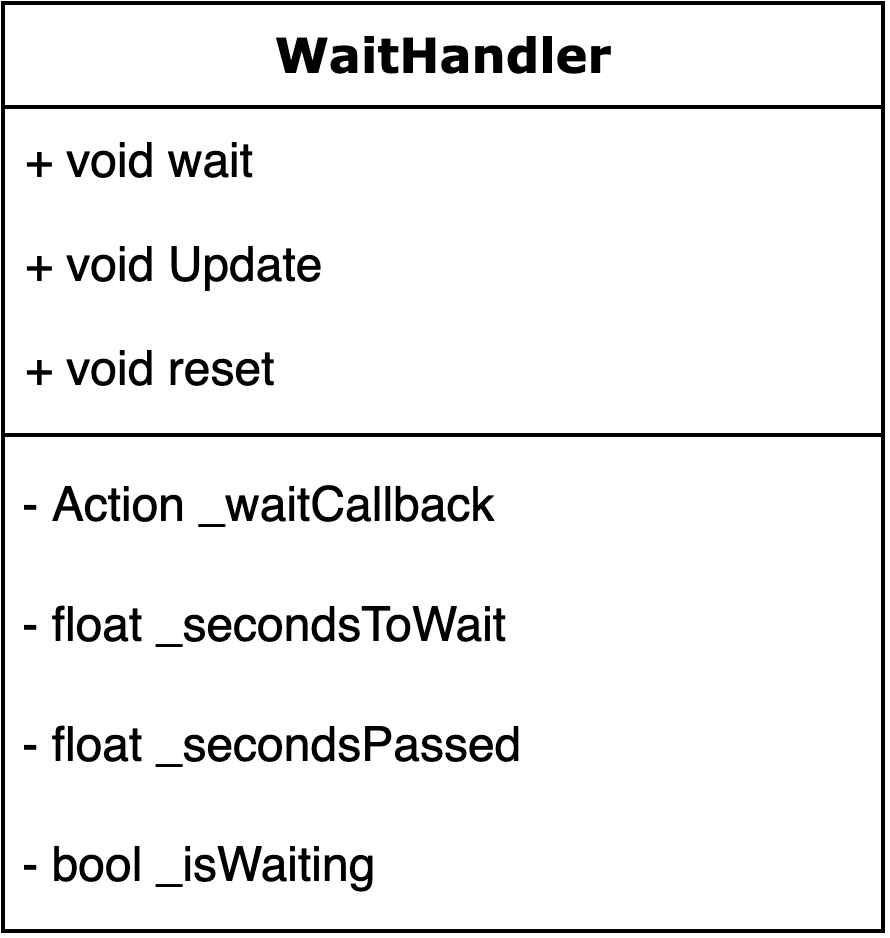
\includegraphics[scale=0.18]{images/village/architecture_diagram_waithandler.png}
\caption{Methoden der Klasse \inlinecode{WaitHandler}}
\label{fig:architecture_diagram_waithandler}
\end{figure}

Eine weitere essentielle Teilaktion ist die \inlinecode{WaitAction}. Diese funktioniert grundsätzlich wie die \inlinecode{MoveAction}, gibt dem zugrunde liegenden \inlinecode{WaitHandler} jedoch kein örtliches Ziel vor, sondern teilt diesem eine Wartezeit mit. Der Aufbau der Klasse \inlinecode{WaitHandler} ist in Abbildung \ref{fig:architecture_diagram_waithandler} zu erkennen.

Durch die Funktion \inlinecode{wait} wird der Wartevorgang eingeleitet. Der Parameter der Funktion bestimmt, wie lange gewartet werden muss. Dieser Wert wird im Feld \inlinecode{\_secondsToWait} gespeichert. Die Variable \inlinecode{\_secondsPassed} sagt aus, wie lange der Wartevorgang bereits andauert. In der Funktion \inlinecode{Update} wird nun \inlinecode{\_secondsPassed} mit \inlinecode{Time.deltaTime} addiert. Sobald gilt, dass \inlinecode{\_secondsPassed >= \_secondsToWait}, wird der Callback \inlinecode{\_waitCallback} aufgerufen und die Variablen der Instanz des \inlinecode{WaitHandler} durch die Funktion \inlinecode{reset} zurückgesetzt. Da \inlinecode{Time.deltaTime} automatisch skaliert wird, funktioniert das Vorgehen auch bei hohen Timescale-Faktoren.



\paragraph{ActionPlans für Berufe}
Die ActionPlans, die berufliche Tätigkeiten darstellen sollen, bauen indirekt aufeinander auf. Durch eine verkettete Beziehung der Ressourcen untereinander entstehen zwischen den einzelnen Ressourcen gewisse Abhängigkeiten. Insgesamt gibt es fünf Endressourcen, die produziert werden müssen: \Fachbegriff{Werkzeuge}, \Fachbegriff{Feuerholz}, \Fachbegriff{Bier}, \Fachbegriff{Fleisch} und \Fachbegriff{Brot}. Für die Herstellung der Werkzeuge muss zunächst ein Minenarbeiter Erz produzieren, welches dann vom Schmied in Werkzeuge verarbeitet werden kann. Für das Feuerholz muss zunächst ein Waldarbeiter Holz hacken, für das Bier muss zunächst Hopfen geerntet und anschließend zu Bier verarbeitet werden und für die Produktion von Fleisch ist zunächst das Jagen von Wild nötig (das nicht dargestellt wird), welches dann zu Fleisch weiterverarbeitet wird. Die einzige Produktionskette mit drei Schritten ist die Herstellung von Brot - erst muss dafür Weizen abgebaut werden, dann muss dieser in der Windmühle zu Mehl verarbeitet und erst dann kann daraus vom Bäcker Brot gebacken werden. Zwischen den ActionPlans besteht kein direkter Zusammenhang, doch falls eine Ressource nicht ausreichend vorhanden ist, kann die Kette unterbrochen werden, sodass ebenfalls weitere Ressourcen nicht hergestellt werden können.
Alle Berufe verbrauchen zudem Werkzeuge. Das gilt nur nicht für Minenarbeiter und Schmiede, da diese die Werkzeuge herstellen.






\paragraph{Übersicht über ausführbare Aktionen}
Es wurden insgesamt 29 ausführbare ActionPlans erstellt, die die Aktionen des Agenten beschreiben. Diese werden durch den \inlinecode{ActionHandler} verwaltet und dort in einem Mapping den Identifiern der Aktionen zugewiesen.

Die ActionPlans werden in die Kategorien \Fachbegriff{Communication}, \Fachbegriff{Education}, \Fachbegriff{Exhaustion}, \Fachbegriff{Hunger}, \Fachbegriff{Recreation}, \Fachbegriff{Religion}, \Fachbegriff{Sleep}, \Fachbegriff{Thirst} und \Fachbegriff{Work} eingeteilt. Für jedes der Bedürfnisse der Agenten gibt es mindestens einen ActionPlan, der dieses Bedürfnis befriedigt.

\smallskip
Das folgende Listing enthält eine kurze Beschreibung der jeweiligen Aktionen.


\begin{table}[H]
\footnotesize
\centering
\begin{tabular} {|  p{4.8cm}  |  p{7.3cm}  |  p{1.8cm}  |  p{0.9cm}|} \hline
\textbf{ActionPlan} & \textbf{Beschreibung} & \textbf{Ort} & \textbf{Dauer} \\ \hline

\inlinecode{CommunicationChatActionPlan} &  Befriedigt Kommunikationsbedürfnis. Agenten treffen sich dafür in Gruppen und kommunizieren. & Markplatz & Kurz \\ \hline
\inlinecode{EducationCollegeActionPlan} & Befriedigt Bildungsbedürfnis. Verfügbar für Agenten zwischen 19 und 35 Jahren. & College & Mittel \\ \hline
\inlinecode{EducationLibraryActionPlan} & Befriedigt Bildungsbedürfnis. Verfügbar für Agenten ab 36 Jahren. & Bibliothek & Mittel \\ \hline
\inlinecode{EducationSchoolActionPlan} & Befriedigt Bildungsbedürfnis. Verfügbar für Agenten zwischen 0 und 18 Jahren. & Bibliothek & Mittel \\ \hline
\inlinecode{ExhaustionRestActionPlan} & Verbessert Erschöpfungslevel des Agenten. & Zuhause & Mittel \\ \hline
\inlinecode{HungerBreadActionPlan} & Befriedigt Hungerdedürfnis und verbraucht Brot. & Markt & Kurz \\ \hline
\inlinecode{HungerMeatActionPlan} & Befriedigt Hungerdedürfnis und verbraucht Fleisch. & Markt & Kurz \\ \hline
\inlinecode{RecreationBarbecueActionPlan} & Freizeitaktion. Agenten treffen sich in Gruppen am Lagerfeuer. & Lagerfeuer & Mittel  \\ \hline
\inlinecode{RecreationCafeActionPlan} & Freizeitaktion. Agent besucht Cafe. & Cafe & Mittel \\ \hline
\inlinecode{RecreationShootingActionPlan} & Freizeitaktion. Agent besucht Schießstand. & Schießstand & Mittel \\ \hline
\inlinecode{RecreationShopActionPlan} & Freizeitaktion. Agent besucht Laden. & Shop & Mittel \\ \hline
\inlinecode{RecreationSoccerActionPlan} & Freizeitaktion. Agent besucht Fußballplatz. & Fußballplatz & Mittel \\ \hline
\inlinecode{RecreationTavernActionPlan} & Freizeitaktion. Agent besucht Taverne. & Taverne & Mittel \\ \hline
\inlinecode{RecreationTheaterActionPlan} & Freizeitaktion. Agent besucht Theater. & Theater & Mittel \\ \hline
\inlinecode{RecreationVisitActionPlan} & Freizeitaktion. Agent besucht Haus eines anderen NPC (Auswahl erfolgt zufällig). & Fremdes Zuhause & Mittel \\ \hline
\inlinecode{ReligionChurchActionPlan} & Befriedigt Glaubensbedürfnis. Agent besucht Kirche. & Kirche & Kurz \\ \hline
\inlinecode{SleepActionPlan} & Befriedigt Schlafbedürfis. & Zuhause & Lang \\ \hline
\inlinecode{ThirstActionPlan} & Befriedigt Durstbedürfis. Der Agent trinkt vom Brunnen. & Brunnen & Sehr Kurz \\ \hline
\inlinecode{WorkBeerBreweryActionPlan} & Befriedigt Arbeitsbedürfis. Agent arbeitet als Braumeister. Verbraucht Hopfen. & Brauerei & Lang \\ \hline
\inlinecode{WorkBeerFarmHopsActionPlan} & Befriedigt Arbeitsbedürfis. Agent arbeitet als Hopfenbauer. & Hopfenfarm & Lang \\ \hline
\inlinecode{WorkBreadBakeryActionPlan} & Befriedigt Arbeitsbedürfis. Agent arbeitet als Bäcker. Stellt Brot her. Verbraucht Mehl. & Bäckerei & Lang \\ \hline
\inlinecode{WorkBreadFarmGrainActionPlan} & Befriedigt Arbeitsbedürfis. Agent arbeitet als Weizenbauer. Stellt Weizen her. & Weizenfarm & Lang \\ \hline
\inlinecode{WorkBreadWindmillActionPlan} & Befriedigt Arbeitsbedürfis. Agent arbeitet als Müller. Stellt Mehl her. Verbraucht Weizen. & Windmühle & Lang \\ \hline
\inlinecode{WorkMeatButcherActionPlan} & Befriedigt Arbeitsbedürfis. Agent arbeitet als Fleischer.  Stellt verarbeitetes Fleisch her. Verbraucht rohes Fleisch. & Fleischerei & Lang \\ \hline
\inlinecode{WorkMeatHuntingActionPlan} & Befriedigt Arbeitsbedürfis. Agent arbeitet als Jäger. Stellt rohes Fleisch her. & Wald & Lang \\ \hline
\inlinecode{WorkToolsBlacksmithActionPlan} & Befriedigt Arbeitsbedürfis. Agent arbeitet als Schmied. Stellt Werkzeuge her. Verbraucht Eisen. & Schmied & Lang \\ \hline
\inlinecode{WorkToolsMiningActionPlan} & Befriedigt Arbeitsbedürfis. Agent arbeitet als Minenarbeitet. Stellt Eisenerz her. & Mine & Lang \\ \hline
\inlinecode{WorkWoodCarpenterActionPlan} & Befriedigt Arbeitsbedürfis. Agent arbeitet als Zimmermann. Stellt Holz her. Verbraucht Holzstämme. & Zimmermann & Lang \\ \hline
\inlinecode{WorkWoodLoggingActionPlan} & Befriedigt Arbeitsbedürfis. Agent arbeitet als Holzfäller. Stellt Holzstämme her. & Wald & Lang \\ \hline

\end{tabular}
\caption{Auflistung aller ActionPlans}
\label{tab:action_plans}
\end{table}







\subsubsection{NpcState}
In der Klasse \inlinecode{NpcState} wird der Zustand des Agenten inklusive seiner Bedürfnisse und Attribute beschrieben. Die Abbildung \ref{fig:architecture_diagram_npcstate} zeigt die Funktionen der Klasse:

\begin{figure}[H]
\centering
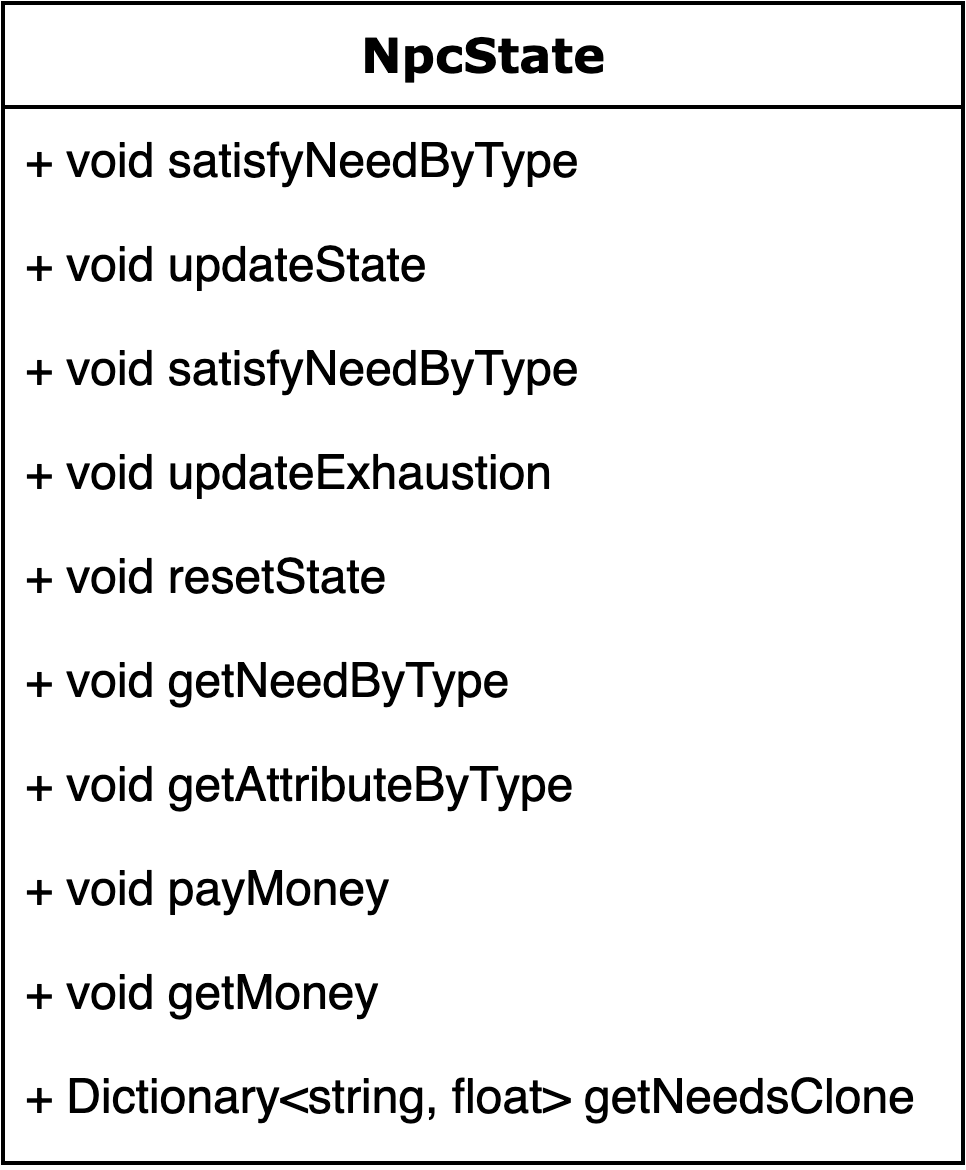
\includegraphics[scale=0.18]{images/village/architecture_diagram_npcstate.png}
\caption{Methoden der Klasse \inlinecode{WaitHandler}}
\label{fig:architecture_diagram_npcstate}
\end{figure}

Die Methoden \inlinecode{payMoney} und \inlinecode{gainMoney} werden genutzt, um die Geldmenge des Agenten zu verändern, beispielsweise wenn eine Aktion als Voraussetzung gewisse Kosten erfordert. Zusätzlich zu den im \inlinecode{ResourceHandler} definierten Ressourcen verfügt der Agent über eine spezielle Ressource \Fachbegriff{Money}, die im \inlinecode{NpcState} definiert wird. Im Gegensatz zu normalen Ressourcen verfügt jeder Agent über einen individuellen Wert für die Geldmenge, die er besitzt. Bestimmte Aktionen sind mit Kosten verbunden, die der Agent bezahlen muss. Geld kann nur durch Arbeits-Aktionen dazugewonnen werden. In einem ActionPlan kann durch die Veränderung der Variable \inlinecode{\_money} ein Wert für die Kosten der Aktion gesetzt werden. Dadurch soll der Agent über den Reward hinaus dazu angeregt werden, zu arbeiten. Außerdem führt dies dazu, dass bestimmte teure Aktionen von bestimmten Bevölkerungsgruppen, die mehr Geld verdienen, bevorzugt werden. Ein Bäcker verdient beispielsweise mehr Geld als ein Bauer.


Es werden einige Funktionen definiert, um Bedürfnisse und Attribute zu aktualisieren und abzufragen. In der Funktion \inlinecode{resetState} findet weiterhin nach dem Abschließen einer Episode ein Zurücksetzen der Werte statt. Da für die verteilte Belohnung in ActionPlans die initialen Bedürfnisse bekannt sind wurde die Funktion \inlinecode{getNeedsClone} implementiert. Sie gibt eine Kopie der aktuellen Werte aller Bedürfnisse zurück, die zu Beginn der Ausführung eines ActionPlans bezogen werden und nach der Ausführung verwendet werden kann.
Die Funktion \inlinecode{updateState} wird vom \inlinecode{TimeController} in regelmäßigen Abständen aufgerufen. Sie aktualisiert den Zustand des Agenten durch die Bereitstellung der neuen aktuellen Zeit und verändert damit seine Bedürfnisse. Die Funktion ist in Abbildung \ref{lst:npcstate_updatestate} zu sehen:

\begin{minipage}{\linewidth}
\begin{lstlisting}[linewidth=16.4cm, label=lst:npcstate_updatestate, caption=Funktion \inlinecode{updateState} in \inlinecode{NpcState}, xleftmargin=1cm, basicstyle=\footnotesize]
public void updateState(float currentTime, float deltaTime) {
    _exhaustion += 0.0002f * deltaTime;

    List<string> needsToUpdate = new List<string>();
    foreach (string needType in _needs.Keys) needsToUpdate.Add(needType);
    foreach (string needType in needsToUpdate) {
        _secondsSinceSatisfaction[needType] += deltaTime;
        _needs[needType] = _needCycleHandler.getUpdatedNeedValue(needType, _secondsSinceSatisfaction[needType]);
        if (_useGoap && _needs[needType] < 0.1f) _goapEffectSetter.setGoapEffect(needType, true);
    }
    _recreation = _needCycleHandler.calculateRecreationValue(_needs);
    _sleep = _needCycleHandler.calculateSleepValue(currentTime);
    _work = _needCycleHandler.calculateWorkValue(currentTime);
}
\end{lstlisting}
\end{minipage}

Neben den Werten für Exhaustion und Recreation (siehe Kapitel \ref{npc_needs_architecture}) werden ebenfalls die Bedürfnisse des Agenten angepasst, indem zusätzliche Funktionen aufgerufen werden. Die Bedürfnisse Schlaf und Arbeit werden dabei gesondert behandelt. Die genaue Funktionsweise der Bedürfnisse wird im folgenden Abschnitt \ref{npc_needs_architecture} behandelt.


\subsubsection{Bedürfnisse}\label{npc_needs_architecture}
Für die Simulationen werden Utility-Based Agents verwendet (siehe Abschnitt \ref{utility_agents}). Konkret werden diese so implementiert, dass sie über verschiedene menschliche Bedürfnisse verfügen. Im \inlinecode{NeedCycleHandler} werden jeweils Funktionen $g_b(x)$ definiert, die diese Bedürfnisse in Abhängigkeit von der verstrichenen Zeit verändern.

Ein Bedürfniswert von $g_b(x) = 1$ bedeutet, dass der Agent hinsichtlich dieses spezifischen Begehrens vollkommen befriedigt ist. Ein Bedürfniswert von $g_b(x) = 0$ hingegen bedeutet, dass der Agent ein starkes Bedürfnis hat, das es zu befriedigen gilt.
Als Grundbedürfnisse werden \textit{Hunger}, \textit{Durst}, \textit{Bildung}, \textit{Kommunikation}, und \textit{Glauben} definiert. Weiterhin gibt es die Bedürfnisse \textit{Schlaf} und \textit{Arbeit}. Im Spiel werden diese als \textit{NEED\_HUNGER}, \textit{NEED\_THIRST}, \textit{NEED\_EDUCATION}, \textit{NEED\_COMMUNICATION}, \textit{NEED\_FAITH}, \textit{SLEEP} und \textit{WORK} implementiert.

Die Werte für die fünf Grundbedürfnisse hängen davon ab, wann das Bedürfnis zuletzt befriedigt wurde. Sie verwenden die folgende Grundfunktion $g_b(x)$:

\begin{minipage}{\linewidth}
\begin{lstlisting}[linewidth=16.4cm, label=lst:village_needs_base_function, caption=Grundfunktion für die Abnahme der Grundbedürfnisse, xleftmargin=1cm]
private float _getFunctionValue(float cycleLengthSeconds, float exponent, float xValue) {
    float baseVal = xValue / cycleLengthSeconds;
    float pow = Mathf.Pow(baseVal, exponent);
    return Mathf.Clamp(1f - pow, 0f, 1f);
}
\end{lstlisting}
\end{minipage}

Für jede der Basisfunktionen $g_b(x)$ werden die in der Grundfunktion verwendeten Parameter wie \inlinecode{exponent}, \inlinecode{baseVal} und \inlinecode{cycleLengthSeconds} eigens definiert. Wenn die Bedürfnisse akutalisiert werden, wird für die Berechnung der einzelnen Werte ein \Fachbegriff{Switch-Case}-Konstrukt verwendet, wie in Listing \ref{lst:village_needs_switchcase} zu sehen.

\begin{minipage}{\linewidth}
\begin{lstlisting}[linewidth=16.4cm, label=lst:village_needs_switchcase, caption=Aufruf der Grundfunktion bei einer Anpassung der Bedürfnisse, xleftmargin=1cm]
public float getUpdatedNeedValue(string needType, float timeSinceSatisfaction) {
    switch(needType) {
        case NpcState.NEED_HUNGER:
            return _getFunctionValue(HUNGER_CYCLE_SECONDS,
                HUNGER_DROP_RATE, timeSinceSatisfaction);
        case NpcState.NEED_THIRST:
            return _getFunctionValue(THIRST_CYCLE_SECONDS,
                THIRST_DROP_RATE, timeSinceSatisfaction);
        [...] // Cases with other needs.
    }
    return -1f;
}
\end{lstlisting}
\end{minipage}


Das folgende Beispiel betrachtet exemplarisch die Hungerfunktion $g_{hunger}(x)$ des Agenten. Wenn die verwendeten Konstanten eingesetzt werden, ergibt sich der folgende Aufruf:

\begin{minipage}{\linewidth}
\begin{lstlisting}[linewidth=16.4cm, label=lst:village_needs_hunger_call, caption=Aufruf der Grundfunktion bei einer Anpassung der Bedürfnisse, xleftmargin=1cm]
_getFunctionValue(
    cycleLengthSeconds = DAY_CYCLE_SECONDS * 0.5f,
    exponent = 2.5f,
    xValue = timeSinceSatisfaction
);
\end{lstlisting}
\end{minipage}

Durch Einsetzen der Werte verändert das die Grundfunktion wie folgt:

\begin{minipage}{\linewidth}
\begin{lstlisting}[linewidth=16.4cm, label=lst:village_needs_base_function_eingesetzt, caption=Grundfunktion für Bedürfnisse (Beispiel Hungerbedürfnis), xleftmargin=1cm]
float baseVal = timeSinceSatisfaction / (DAY_CYCLE_SECONDS * 0.5f);
float pow = Mathf.Pow(baseVal, 2.5f);
return Mathf.Clamp(1f - pow, 0f, 1f);
\end{lstlisting}
\end{minipage}

Nun ist leicht zu sehen, dass sich folgende mathematische Funktion daraus ergibt: 

$$ g_{hunger}(x) = 1 - {(x / 500)}^2.5 $$

Die Funktionen für das Schlaf- und Arbeitsbedürfnis wurden anhand von Abbildung \ref{fig:village_diagram_hunger-function} visualisiert. Für die Variable \inlinecode{DAY\_CYCLE\_SECONDS}, die den Tageszyklus bestimmt. wird dabei eine Dauer von 1000 Sekunden genutzt.

\begin{figure}[H]
\centering
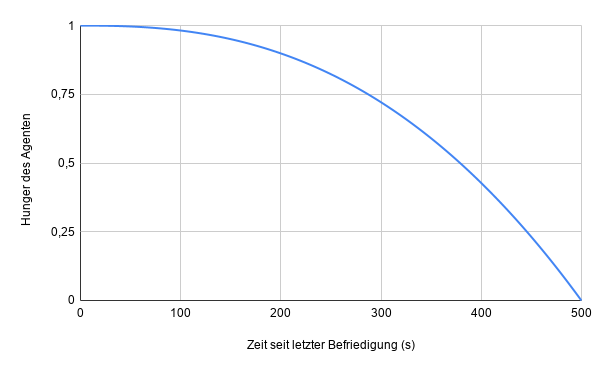
\includegraphics[scale=0.7]{images/village/village_diagram_hunger-function.png}
\caption{Hungerfunktion des Agenten}
\label{fig:village_diagram_hunger-function}
\end{figure}

Die Bedürfnisse \Fachbegriff{Schlaf} und \Fachbegriff{Arbeit} verhalten sich anders. Diese sind nicht davon abhängig, wann das Bedürfnis das letzte mal befriedigt wurde, sondern hängen von der Tageszeit ab. Das Listing \ref{lst:village_sleep_function} zeigt, wie das Schlafbedürfnis berechnet wird.

\begin{minipage}{\linewidth}
\begin{lstlisting}[linewidth=16.4cm, label=lst:village_sleep_function, caption=Funktion für das Schlafbedürfnis, xleftmargin=1cm]
public float calculateSleepValue(float currentTime) {
    float baseOffsetX = -0.125f;

    bool exceedsBorders = _exceedsBorders(0.125f - baseOffsetX, 0.625f - baseOffsetX, currentTime);
    if (!exceedsBorders) return 1f;

    float frequency = 4f * Mathf.PI;
    float offset = currentTime + baseOffsetX;
    float funcRes = Mathf.Sin(frequency * offset) * 0.5f + 0.5f;
    return Mathf.Clamp(funcRes, 0f, 1f);
}
\end{lstlisting}
\end{minipage}

Daraus ergibt sich folgende Funktion:

$$ g_{sleep}(x) =  \sin{(4 \pi * (x - 0.125))} * 0.5 + 0.5  $$

Diese Funktionen werden als Basis für eine partielle Funktion verwendet. Die Funktion \inlinecode{\_exceedsBorders} prüft, ob die Werte der X-Achse bestimmte Grenzen überschreiten. Falls dies der Fall ist, wird der Funktionswert nicht durch die oben definierten Funktionen berechnet, sondern entspricht automatisch dem Wert $1$. Die Intervalle, die diese Grenzen für das Schlaf- und Arbeitsbedürfnis definieren, heißen $I_{sleep}$ bzw. $I_{work}$.

$$ g_{sleep}(x)= \left\{
    \begin{array}{ll}
        x \in I_{sleep},     \;\;\;     \sin{(4 \pi * (x - 0.125))} * 0.5 + 0.5     \\
        x \not\in I_{sleep}, \;\;\;   1
    \end{array}
\right.  $$

Die Berechnung des Arbeitsbedürfnis verläuft auf die gleiche Art und Weise. Hier wird lediglich der Offset in der Funktion anders berechnet, wie in Listing \ref{lst:village_work_function_offset} zu sehen. In das Offset wird die Schlafdauer des Agenten mit einbezogen und ein zusätzliches Offset einberechnet. Der Agent soll idealerweise morgens aufwachen und nach kurzer Zeit einen Zuwachs seines Arbeitsbedürfnisses verspüren.

\begin{minipage}{\linewidth}
\begin{lstlisting}[linewidth=16.4cm, label=lst:village_work_function_offset, caption=Berechnung des Offset für das Arbeitsbedürfnis, xleftmargin=1cm]
float sleepDuration = SleepActionPlan.SLEEP_DURATION_HOURS / 24f;
float baseOffsetX = -0.125f - sleepDuration - WORK_SLEEP_OFFSET;
\end{lstlisting}
\end{minipage}

Für das Arbeitsbedürfnis ergibt sich folgende Funktion:

$$ g_{work}(x)= \left\{
    \begin{array}{ll}
        x \in I_{work},     \;\;\;     \sin{(4 \pi * (x - O_{sw}))} * 0.5 + 0.5     \\
        x \not\in I_{work}, \;\;\;   0
    \end{array}
\right.  $$
\begin{centering}  wobei $ O_{sw} = -0.125f - sleepDuration - WORK\_SLEEP\_OFFSET $  \end{centering}
\bigskip

$O_{sw}$ beschreibt den Offset zwischen Werten der Schlaf- und der Arbeitsfunktion.
$g_{work}(x)$ und $g_{sleep}(x)$ können nun berechnet werden. Sie können in Abbildung \ref{fig:village_diagram_sleep_work_functions} betrachtet werden.

\begin{figure}[H]
\centering
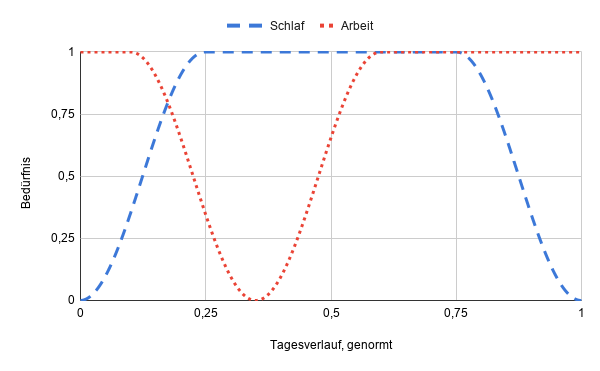
\includegraphics[scale=0.7]{images/village/village_diagram_work_sleep_functions.png}
\caption{Bedürfnisfunktionen des Agenten für Arbeit und Schlaf}
\label{fig:village_diagram_sleep_work_functions}
\end{figure}


Für die Berechnung der Schlaf- und Arbeitsfunktion wird weiterhin ein für jeden Agenten unterschiedlicher Wert verwendet. Bei der Initialisierung des Agenten wird dem Feld \inlinecode{\_rythmVariation} ein zufälliger Wert zugewiesen, um jedem Agenten einen leicht versetzten Rhytmus zu verleihen. Die maximale Amplitude dieses Werts kann durch eine Anpassung der Variable \inlinecode{agentRythmVariation} in der Klasse \inlinecode{GameAcademy} gesteuert werden. Ohne disen OFfset kann es dazu kommen, dass viele - oder alle - Agenten zur selben Zeit schlafen bzw. arbeiten gehen und sich identische Tagesabläufe abbilden.

Zusätzlich zu den genannten Bedürfnissen wurden ein \Fachbegriff{Recreation}-Wert und ein \Fachbegriff{Exhaustion} eingeführt. Der Recreation-Wert ist für das Auslösen von Freizeitaktivitäten verantwortlich. Er berechnet sich wie folgt:

\begin{minipage}{\linewidth}
\begin{lstlisting}[linewidth=16.4cm, label=lst:village_recreation_function, caption=Berechnung des Recreationwerts, xleftmargin=1cm]
public float calculateRecreationValue(Dictionary<string, float> needs) {
    float recreationValue = 0f;
    foreach (string needType in needs.Keys)
    {
        float need = needs[needType];
        if (need < BaseActionPlan.NEED_PENALTY_THRESHOLD) recreationValue += (1f - need) * 100;
        else if (need < 0.3f) recreationValue += (1f - need) * 10f;
        else if (need < 0.4f) recreationValue += (1f - need) * 3f;
        else recreationValue += 1f - need;
    }
    recreationValue = recreationValue / needs.Count / 1.5f;
    return Mathf.Clamp(recreationValue, 0f, 1f);
}
\end{lstlisting}
\end{minipage}

Recreation ist also abhängig von allen Grundbedürfnissen des Agenten. Je \sogenannt{glücklicher} ein Agent ist, also je höher die Werte seiner Grundbedürfnisse sind, desto niedriger ist der Recreationwert. Sobald ein Agent hinsichtlich all seiner Bedürfnisse befriedigt ist, soll er durch einen dann niedrigen Recreationwert Freizeitaktivitäten nachgehen.

Exhaustion wird verwendet, um die Erschöpfung des Agenten zu simulieren. Der Exhaustionwert wird mit jeder \Fachbegriff{MoveAction} und durch das Arbeiten reduziert. Der Wert kann durch Ausruhen, Schlafen oder langes Warten wieder aufgefüllt werden.


\subsubsection{Navigation}\label{agent_navigation}
Während der \inlinecode{LocationHandler} für die Auswahl von Gebäuden zuständig ist und dahingehend Zielpositionen zur Verfügung stellt, ist der \inlinecode{MoveHandler} für die tatsächliche Navigation der Agenten verantwortlich. Dafür wird ein sogenannter \Fachbegriff{NavMeshAgent} verwendet \cite{unity_navmeshagent}. Es handelt sich dabei um ein Feature, das lediglich in der kommerziellen Pro-Version von Unity nutzbar ist. Der \Fachbegriff{NavMeshAgent} nutzt ein \Fachbegriff{NavMesh}, das vorher generiert werden muss. Die Vorberechnung des NavMesh nennt sich \Fachbegriff{Baking}. Das NavMesh ist eine abstrakte Datenstruktur aus zweidimensionalen Polygonen, die für die Wegfindung des Agenten genutzt wird \cite{unity_navmesh}. Es definiert Flächen, die von einem Agenten traversiert werden können. Um Wege zwischen den Polygonen des NavMesh zu finden, können klassische Pathfinding-Algorithmen wie A* verwendet werden. Durch die Verwendung performanter Algorithmen und der Vorberechnung des NavMesh verläuft das Pathfinding sehr effektiv. Im weiteren Verlauf wird angenommen, dass das gesamte NavMesh in der Simulation statisch ist. Kollisionen von Agenten mit der Umgebung kommen daher nicht vor. Weiterhin werden Kollisionen von Agenten untereinander ignoriert.

\begin{figure}[H]
\centering
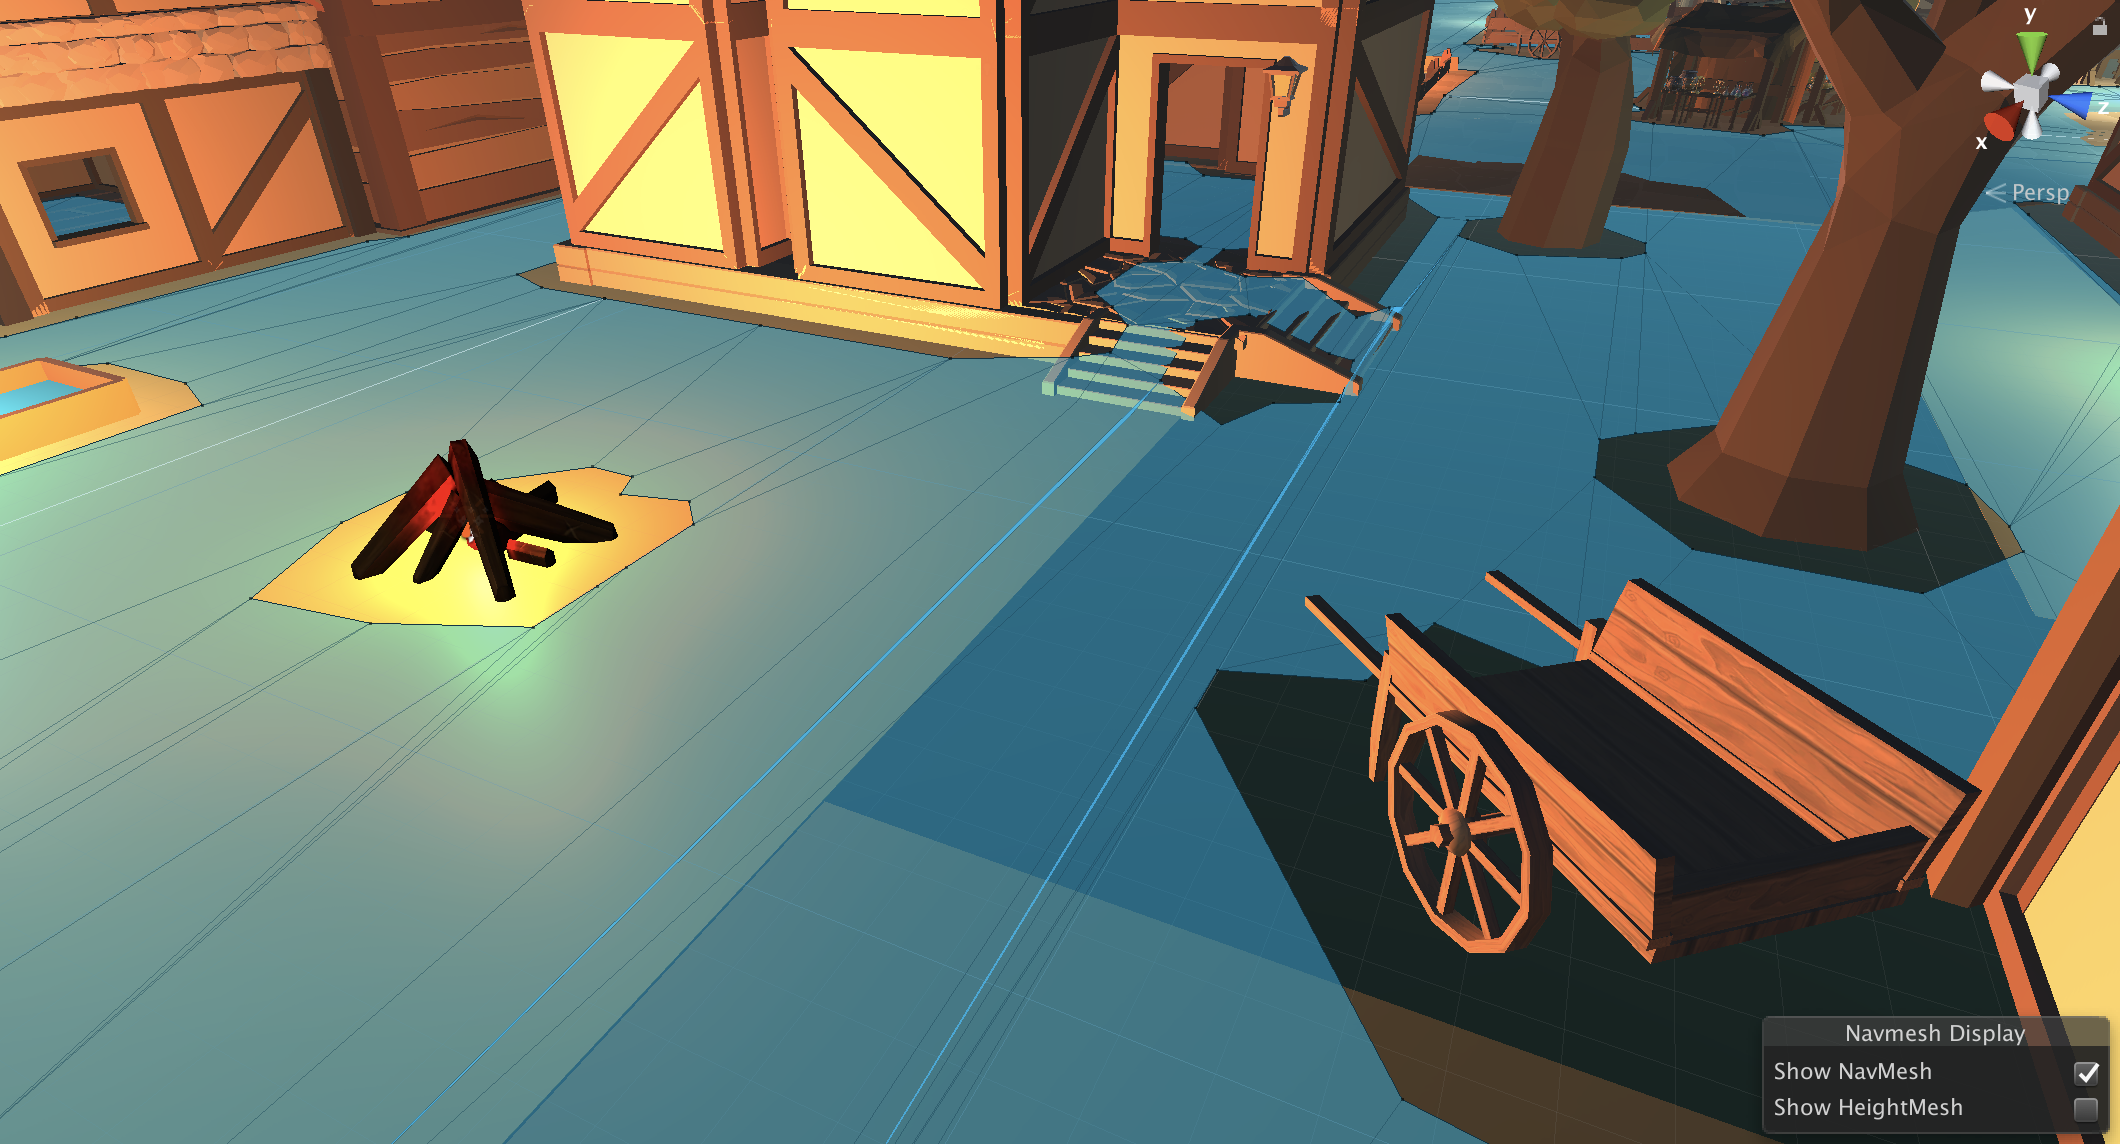
\includegraphics[scale=0.4]{images/village/village_navmesh_1.png}
\caption{Beispielhafter Ausschnitt des generierten NavMesh}
\label{fig:village_navmesh_1}
\end{figure}

Abbildung \ref{fig:village_navmesh_1} zeigt einen beispielhaften Ausschnitt aus dem für die Dorfsimulation generierten NavMesh. Auf der Abbildung ist gut zu erkennen, dass nicht-begehbare Objekte das NavMesh unterbrechen. Beispielsweise bilden der Karren im Vordergrund sowie die Bäume, die Häuser oder das Lagerfeuer Einschnitte in das NavMesh.
Um das NavMesh zu erzeugen, muss für Objekte gekennzeichnet werden, ob sie in die Berechnung mit einbezogen werden oder nicht. Für die Generierung müssen weiterhin einige Parameter gesetzt werden, die die Maße des Agenten beschreiben, sodass Abstände korrekt berücksichtigt werden. Außerdem muss festgelegt werden, wie hoch der Agent springen und welche Steigungen er überwinden kann. Im hinteren Teil der Abbildung \ref{fig:village_navmesh_1} ist dies anhand der Treppe gut zu erkennen. Das blaue NavMesh liegt ebenfalls über der Treppe, weil ihre Steigung vergleichsweise gering ist, sodass der Agent sie ohne weiteres erklimmen kann. Für die Berechnung des NavMesh wurde die Voxelgröße auf 0,125 festgelegt, was bei einem Agentenradius von 0,6 Einheiten 4,8 Voxeln pro Agentenradius entspricht. Dieser Parameter steuert effektiv die Auflösung des NavMesh. Bei der gewählten Größe benötigt die Berechnung, bzw. der \Fachbegriff{Baking}-Vorgang, für ein einzelnes Dorf etwa 30 Sekunden. Um das NavMesh zu nutzen, muss nach erfolgreicher Generierung des NavMesh die Komponente NavMeshAgent an den zu steuernden Agenten angefügt werden. Eine Menge von Einstellungen wie die Geschwindigkeit und Beschleunigung des Agenten können darin gewählt werden.

Der \inlinecode{MoveHandler} hat die Aufgabe, dem NavMeshAgent ein Ziel zu geben. Über die Funktion \inlinecode{moveAgent}, welche als Parameter unter anderem eine Zielposition erhält, wird ein Pfad zum ausgewählten Ziel berechnet und die Wegfindung des Agenten gestartet. Für jeden neuen Frame prüft anschließend die Update-Methode der Klasse, ob das Ziel des Agenten erreicht wurde. Sobald dies der Fall ist wird eine Callbackfunktion aufgerufen, welche die Move-Aktion des Agenten abschließt und die nächste auszuführende Aktion des entsprechenden ActionPlans startet. Die Abbildung \ref{fig:village_navmesh_2} zeigt einige Agenten, die über das NavMesh navigieren.

\begin{figure}[H]
\centering
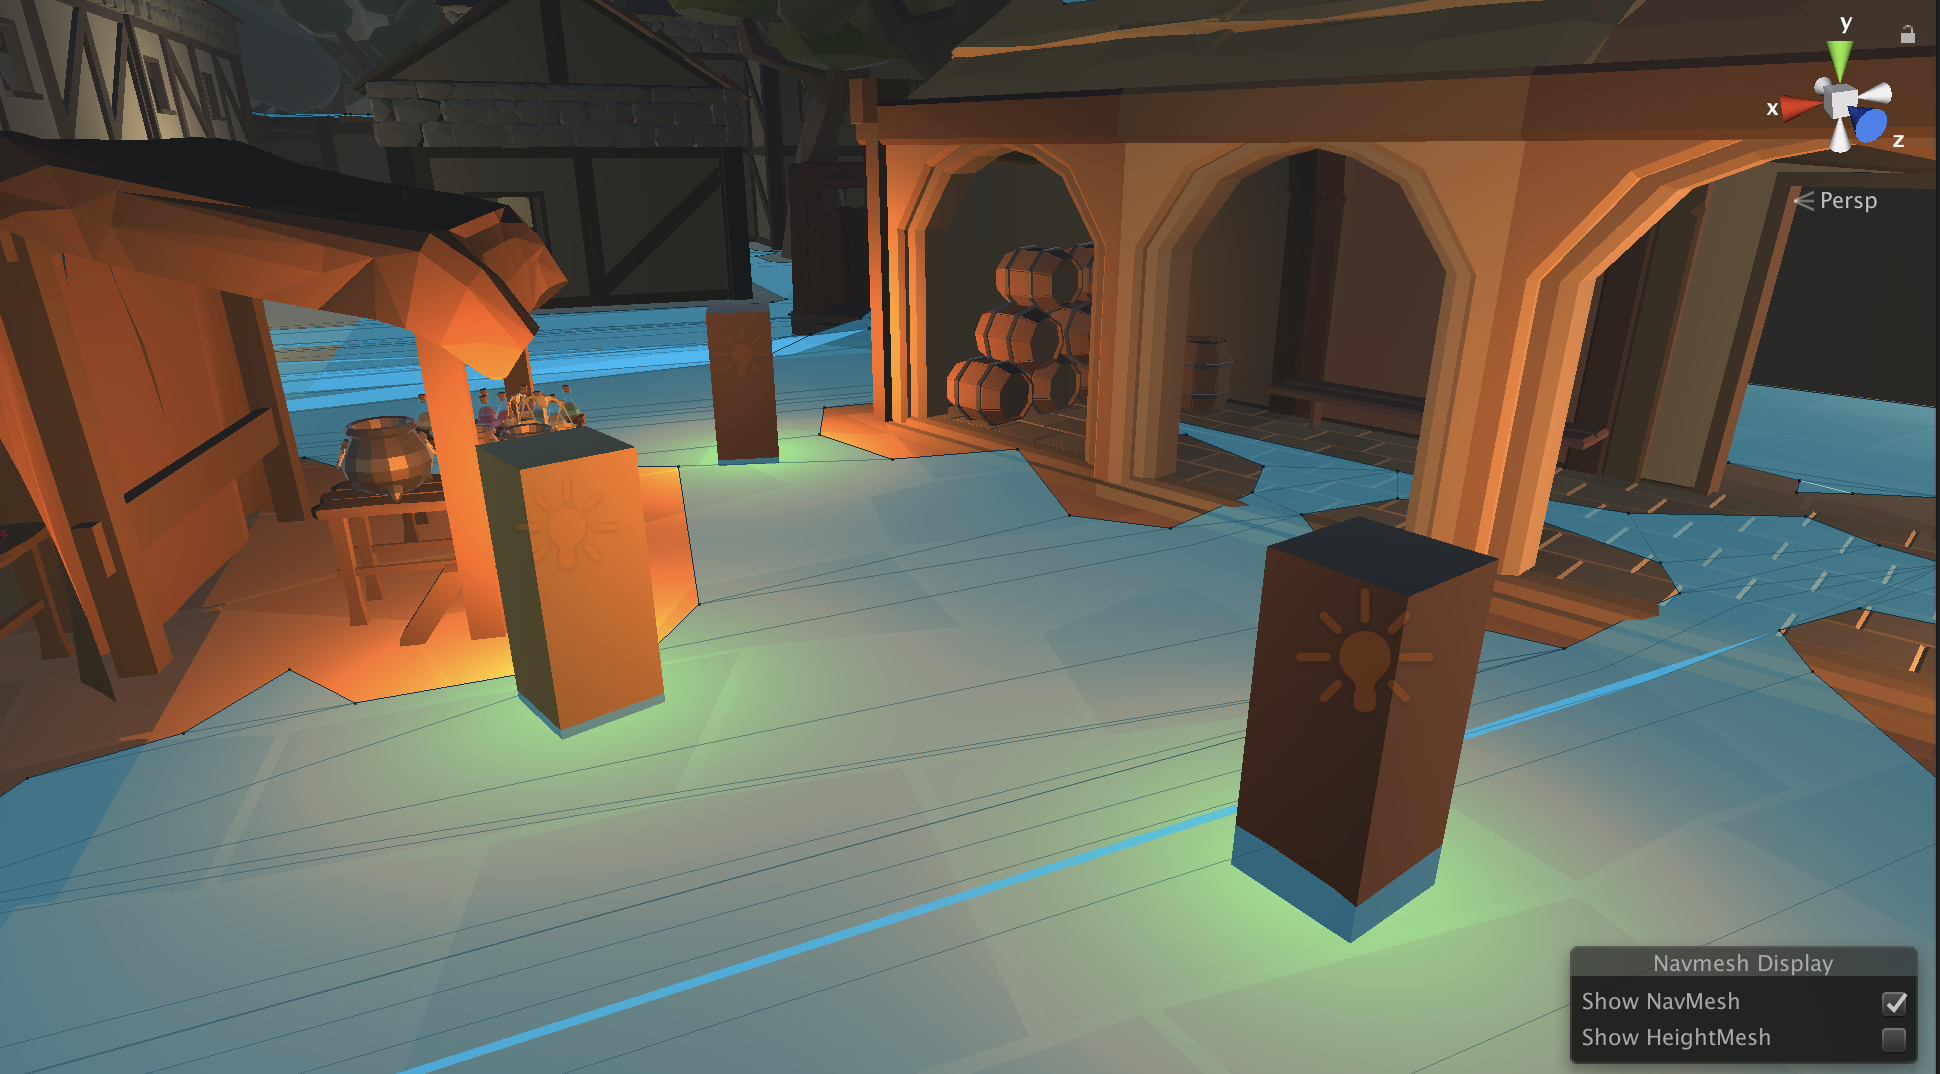
\includegraphics[scale=0.4]{images/village/village_navmesh_2.png}
\caption{Agenten navigieren über das NavMesh}
\label{fig:village_navmesh_2}
\end{figure}


\subsubsection{Maskieren von Aktionen}
Die Größe des Aktionsraum des Agenten ändert sich mit dem Simulationszustand und den Parametern des Agenten. Nicht zu jeder Zeit sind alle Aktionen ausführbar. Stattdessen ist jeder ActionPlan, den der Agent ausführen kann, an bestimmte Bedingungen geknüpft. ML-Agents bietet die Möglichkeit, Aktionen zu \Fachbegriff{maskieren}. Das bedeutet, dass diese Aktionen bei der Entscheidungsfindung nicht in Erwägung gezogen werden. Das neuronale Netz liefert also garantiert einen Output, bei dem die maskierten Aktionen nicht gewählt werden.
Die Erzeugung der \Fachbegriff{ActionMask} ist im folgenden Listing \ref{lst:village_action_mask_creation} erkennbar.

\begin{minipage}{\linewidth}
\begin{lstlisting}[linewidth=16.4cm, label=lst:village_action_mask_creation, caption=Erzeugung der \Fachbegriff{ActionMask} für Aktionen, xleftmargin=1cm]
_actionMask = new List<string>();

foreach (string actionId in NpcActions.ALL_ACTIONS) {
    if (!_actionHandler.areRequirementsMet(actionId)) _actionMask.Add(actionId);
}
\end{lstlisting}
\end{minipage}

Im Abschnitt \ref{action_plans} wurde bereits beschrieben, wie Aktionen mit String-Identifiern verbunden werden. Die Maskierung wird im \inlinecode{ActionMaskingHandler} vorgenommen. Der Aufbau dieser Klasse ist in der folgenden Abbildung \ref{fig:architecture_diagram_actionmaskinghandler} zu erkennen:

\begin{figure}[H]
\centering
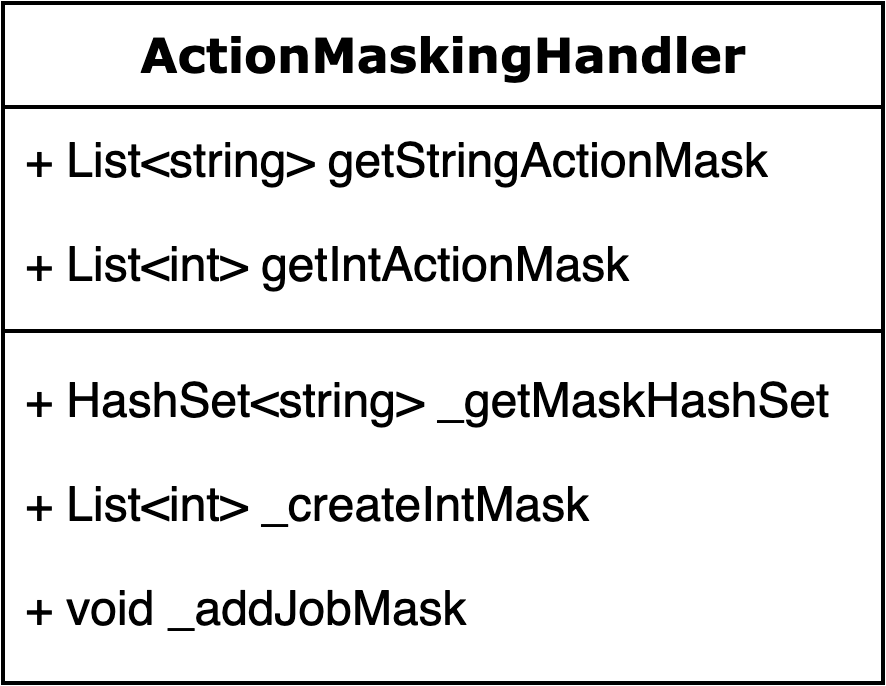
\includegraphics[scale=0.18]{images/village/architecture_diagram_actionmaskinghandler.png}
\caption{Methoden der Klasse \inlinecode{ActionMaskingHandler}}
\label{fig:architecture_diagram_actionmaskinghandler}
\end{figure}

Die eigentliche Erzeugung der ActionMask geschieht in der Funktion \inlinecode{\_getMaskHashSet}. Der \inlinecode{ActionMaskingHandler} iteriert dort über die Identifier aller möglichen Aktionen. Über den Identifier der Aktion erhält dieser vom \inlinecode{ActionHandler} den jeweiligen ActionPlan und ruft dessen Funktion \inlinecode{areRequirementsMet} auf. Wenn eine oder mehrere Bedingungen nicht zutreffen, wird die Aktion maskiert, sodass sie nicht ausgeführt wird. Es wird ein \inlinecode{HashSet<string>} verwendet, welches wie ein Dictionary funktioniert, in dem jedem Schlüssel nur ein einzelner Wert zugewiesen werden kann. Maskierte Aktionen können daher nur einmal in der Kollektion vorkommen - dies wird von ML-Agents gefordert.
Weiterhin wird für das Maskieren ein numerischer Identifier erwartet. Für spätere Verfahren werden hingegen Identifier in Form von \inlinecode{string}s erwartet. Daher wird ein umgekehrtes Mapping verwendet, das aus den String-Identifiern erneut numerische Identifier erzeugt. Weiterhin wird ein Wert vom Typ \inlinecode{List} statt \inlinecode{HashSet} erwartet. Für das Abfragen von integerbasierten oder stringbasierten ActionMasks gibt es daher die Funktionen \inlinecode{getStringActionMask} und \inlinecode{getIntActionMask}.


\subsubsection{Ausführungsfluss des Agenten}
Während der Durchführung von Aktionen interagiert der Agent mit einer Reihe verschiedener Komponenten. Die Architektur des Ausführungsflusses lässt sich anhand eines Komponentendiagramms beschreiben, wie in Abbildung \ref{fig:architektur_agent} zu sehen.

Das Diagramm dient als ergänzende Beschreibung zusätzlich zur generellen Architekturübersicht in Abbildung \ref{fig:architecture_general} und zeigt daher Gemeinsamkeiten. Hier wird jedoch mehr ins Detail gegangen und es besteht ein näherer Bezug zum Agenten selbst.

\bigskip
\begin{figure}[H]
\centering
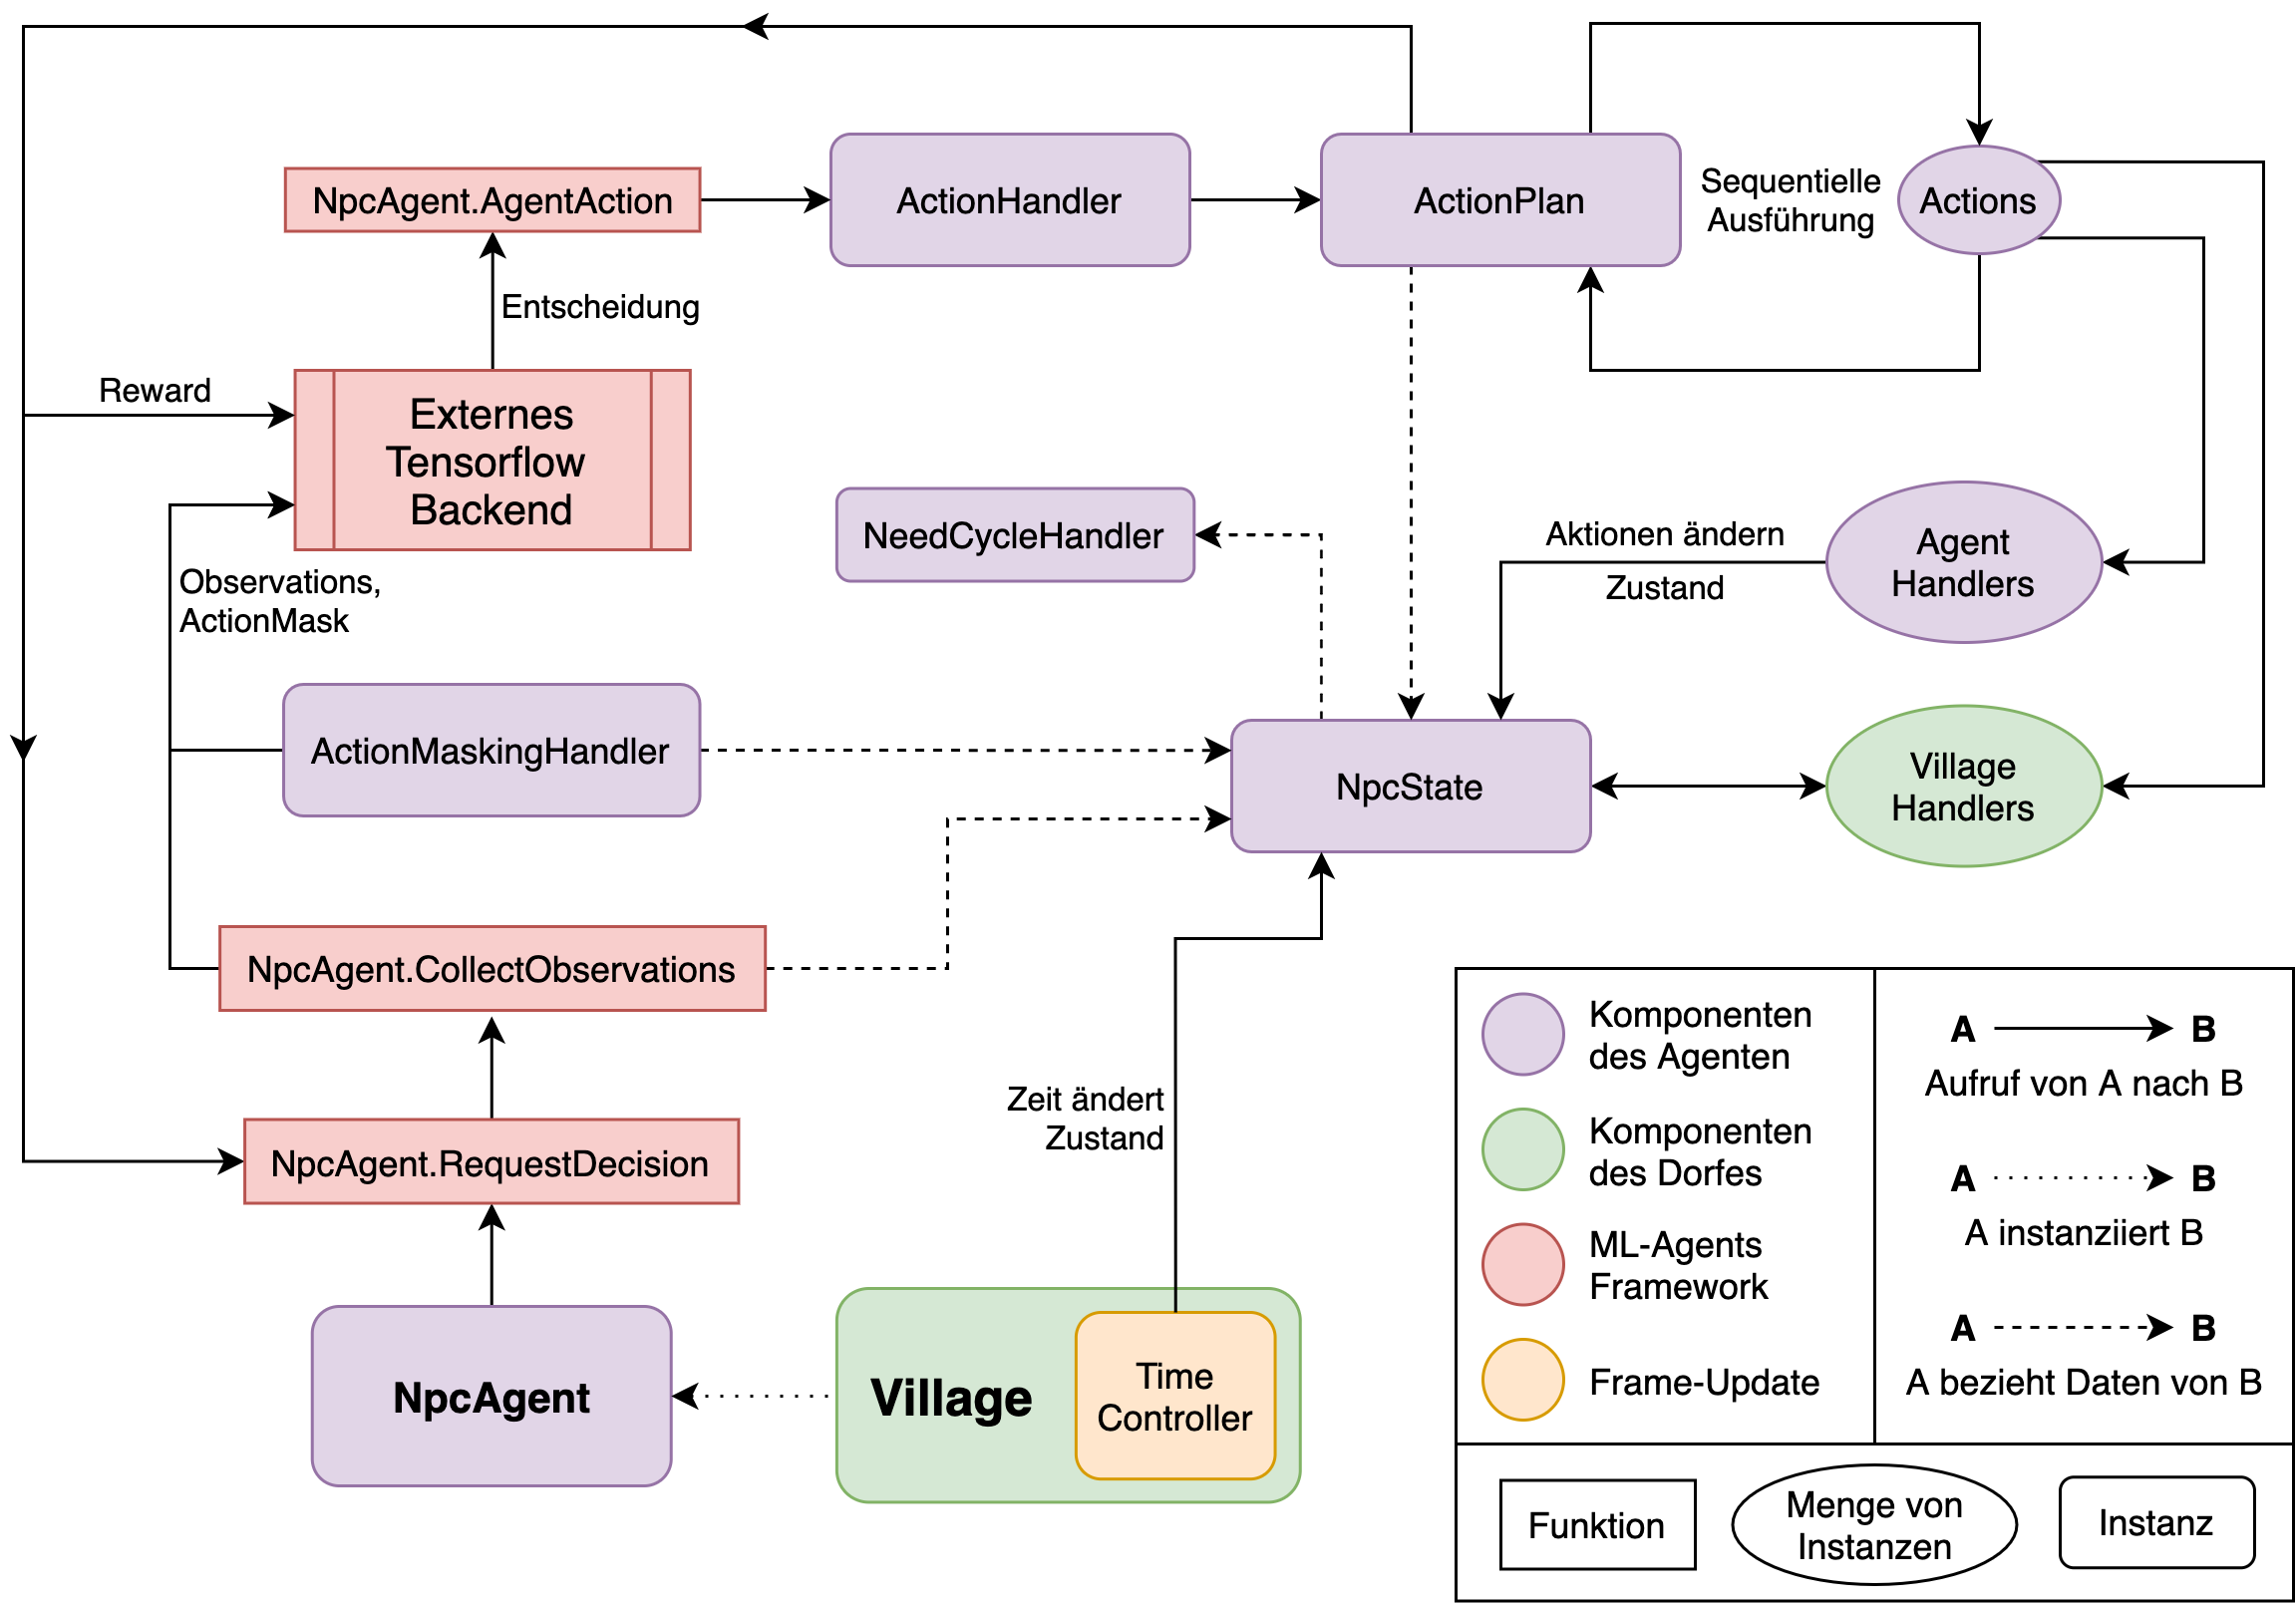
\includegraphics[scale=0.20]{images/village/Master-Thesis_Diagram_Architecture_3.png}
\caption{Architektur der Agenten}
\label{fig:architektur_agent}
\end{figure}

Als erstes sammelt der \ac{npc} eine Menge von Observations. Für die Observations wird der \inlinecode{NpcState} konsultiert. Weiterhin wird der \inlinecode{ActionMaskingHandler} aufgerufen, um den Aktionsraum zu begrenzen. ActionMask und Observations werden dann über die Verbindung des ML-Agents-Frameworks zum externen Tensforflow-Backend geschickt. Als Antwort darauf erhält der Agent eine neue Aktion. Die Funktion \inlinecode{AgentAction} wird aufgerufen und stellt die neue Aktion bereit. Diese wird durch den \inlinecode{ActionHandler} behandelt, der den entsprechenden ActionPlan bereitstellt. Nun werden die einzelnen Sub-Aktionen des ActionPlans ausgeführt. In der Regel sind das \Fachbegriff{Move}- und \Fachbegriff{Wait}-Aktionen. Weitere Aktionen werden in diesem Diagramm vernachlässigt. Die Move-Aktionen werden durch den \inlinecode{MoveHandler} ausgeführt, der mit dem \inlinecode{LocationHandler} kommuniziert. Der \inlinecode{WaitHandler} führt die Wait-Aktionen aus.
Wenn der Agent schließlich alle Sub-Aktionen ausgeführt hat, wird der \inlinecode{NpcState} aktualisiert. Aktionen haben Auswirkungen sowohl auf den Zustand des Agenten als auch unter Umständen auf den Zustand des Dorfes. Die neuen Bedürfnisse werden vom \inlinecode{NeedCycleHander} berechnet. Ressourcen werden aktualisiert und Bedürfnisse angepasst oder zurückgesetzt. Außerdem wird der \inlinecode{MonitorHandler} mit neuen Werten aus dem \inlinecode{NpcState} aktualisiert, um im HUD der Simulation aktuelle Werte anzuzeigen.
Außerdem wird eine Belohnung bzw. Bestrafung für die Aktion verteilt. Über eine Callbackfunktion im ActionPlan schließt sich der Ausführungskreislauf. Eine neue Aktion wird durch den Agenten gestartet, indem \inlinecode{RequestDecision} aufgerufen wird.
Zusätzlich zu diesem Ausführungsablauf wird in regelmäßigen Abständen die Update-Funktion der Komponente \inlinecode{TimeController} des Moduls \inlinecode{Village} aufgerufen, welche die Zustände aller Agenten verändert, indem sich durch das Voranschreiten der Zeit deren Bedürfnisse verändern.











\subsubsection{Belohnungen}\label{agents_rewards}
Die Belohnungen des Agenten hängen grundsätzlichen von seinen Bedürfnissen und dem Zweck der Aktion ab. Sie werden jeweils am Ende einer Aktionen verteilt und in den ActionPlans definiert. Jeder ActionPlan ist mit einem bestimmten Bedürfnis des Agenten verbunden, das durch ihn befriedigt wird. Die Berechnung der Belohnung berücksichtigt, wie ausgeprägt dieses bestimmte Bedürfnis zum Zeitpunkt der Ausführung war. Wenn der Agent beispielsweise sehr hungrig ist, also etwa einen Hungerwert $g_{hunger} = 0$ hat und eine Aktion \Fachbegriff{Essen} auswählt, welche das Hungergefühl stillt, so wird er eine hohe Belohnung bekommen. Wenn er bereits vollkommen gesättigt ist ($g_{hunger} = 1$) und die Aktion \Fachbegriff{Essen} auswählt, wird er eine Bestrafung erhalten. Der Agent soll dadurch lernen, Aktionen zu wählen, die seine Bedürfnisse sinnvoll befriedigen. Wenn alle Bedürfnisse befriedigt sind hat der Agent einen niedrigen Recreationwert, sodass er Freizeitaktivitäten nachgehen kann. Die Belohnungen funktionieren hier auf eine ähnliche Art und Weise. Dies ist ebenfalls beim Arbeits- und Schlafbedürfnis der Fall, obwohl diese Bedürfnisse nicht durch die Aktion aufgefüllt werden, sondern von der Tageszeit abhängen.


Die Belohnungen bestimmter Aktionen hängen außerdem von den Attributen der Agenten ab. Um den Agenten eine Persönlichkeit zu verleihen, werden Attribute wie \Fachbegriff{Intelligence}, \Fachbegriff{Companionship} oder \Fachbegriff{Fitness} im \inlinecode{NpcState} festgelegt.
Dadurch sollen allgemeine Unterschiede zwischen den Agenten, aber auch Unterschiede zwischen verschiedenen Gruppen von Agenten entstehen. Diese Gruppen werden durch die Berufe der Agenten bestimmt. Grundsätzlich werden die Attribute zufällig verliehen, zusätzlich wird bestimmten Berufen die Tendenz gegeben, bei bestimmten Attributen durchschnittlich höhere Werte zu erzielen als andere Berufe. Die Verleihung von Attributen aufgrund des Berufs spiegelt nicht die realen Welt, sondern wurde willkürlich festgelegt. Die Festlegung dieser Attribute wird in der statischen Klasse \inlinecode{AttributeHandler} durchgeführt. Die statische Methode \inlinecode{getAttributesByJobId} erhält als Parameter einen Identifier für den Job des Agenten und gibt ein \inlinecode{Dictionary<string,float>} mit den jeweiligen Attributen zurück. In einer \inlinecode{switch-case}-Anweisung werden die Attribute aufgrund des Berufs vergeben. Die Funktion wird vom \inlinecode{NpcState} aufgerufen.
Beispielsweise wird im ActionPlan \inlinecode{RecreationTavernActionPlan} eine Freizeitaktion definiert, die Agenten besuchen dabei die Taverne. Die Belohnung der Aktion skaliert invertiert mit dem Fitness- und Intelligenzlevel des \ac{npc}. Je niedriger die Fitness- und Intelligenzattribute des Agenten sind, desto höher fällt die Belohnung aus. So kommt es dazu, dass man mehr Minenarbeiter als Jäger in der Taverne antrifft, weil diese durchschnittlich über einen niedrigen Fitnesslevel sowie einen leicht niedrigeren Intelligenzlevel verfügen. Jäger werden mit einem überdurchschnittlich hohen Fitnesslevel häufiger auf dem Fußballplatz statt in der Taverne angetroffen. Beim Training werden diese Gegebenheiten durch die Veränderung des Rewards automatisch in den Lernvorgang mit einbezogen.

Für die Festlegung von Belohnung werden unter anderem die Hilfsfunktionen \inlinecode{\_getNeedReward}, \inlinecode{\_getRecreationReward}, \inlinecode{\_getNeedReward} der Klasse \inlinecode{BaseActionPlan} und die Funktion \inlinecode{\_getWorkReward} der Klasse \inlinecode{WorkActionPlan} verwendet. Mithilfe von Funktionen wie \inlinecode{\_calculateAttributeMultReward} werden Multiplikatoren für die Attribute berechnet, um die Belohnungen negativ oder positiv zu beeinflussen.
Weiterhin wird für sämtliche Belohnungen, die am Ende einer Aktion ausgeführt wurden, stets die Werte des Zustands des Agenten verwendet, die zum Anfang der Ausführung der Aktion vorhanden waren. Dadurch wird verhindert, dass der berechnete Reward direkt mit den vorher gesammelten Observations des Agenten übereinstimmen und eine Beziehung aufgebaut werden kann.











%  Der \inlinecode{JobHandler} ist unter anderem dafür zuständig, den Agenten in Abhängigkeit von den aktuell verfügbaren Ressourcen Berufe zuzuweisen.
\subsection{VillageAgent}\label{village_village_agent}
Den Agenten werden bei der Initialisierung Berufe zugewiesen. Für die Behandlung der Berufe der Agenten können mit der Anpassung des Parameters \inlinecode{ignoreJobMask} der Klasse \inlinecode{GameAcademy} zwei Modi gewählt werden. Der Parameter wurde eingeführt da sich beim Training herausgestellt hat, dass die Wahl der beruflichen Aktionen der Agenten eine Schwierigkeit darstellt.

Wenn der Parameter gesetzt ist wird der Beruf des Agenten ignoriert. Der Aktionsraum eines jeden Agenten verfügt dann über alle möglichen Berufsaktionen. Es wird also jeweils die berufliche Aktion gewählt, die für den Agenten voraussichtlich die höchste zukünftige Belohnung zuweist. Dadurch soll gewährleistet werden, dass das Ressourcensystem in einem stabilen Zustand gehalten wird, da das Ressourcenmanagement durch die Auswahl der beruflichen Aktivitäten der Agenten automatisch in einer Balance gehalten wird. Wenn von einer benötigte Ressource nur noch geringe Mengen vorhanden sind, sollten Agenten automatisch den Beruf ausführen, der die entsprechende Ressource herstellt. Die Agenten müssen in diesem Fall also Observations über die vorhandenen Ressourcen sammeln.    

Wenn der Parameter \inlinecode{ignoreJobMask} nicht gesetzt wird werden hingegen alle Jobs, die nicht dem Job des Agenten entsprechen, permanent maskiert und deren Ausführung dadurch blockiert. Der Agent hat dann also einen festen Job und wird von allen weiteren Jobs ausgeschlossen. Vor dem Trainingsvorgang ist allerdings nicht bekannt, wie viele Agenten welchen Job ausführen müssen, um eine Balance im Ressourcensystem herzustellen, wie oben beschrieben. Die Agenten müssen in diesem Fall keine Observations über die vorhandenen Ressourcen sammeln, da ohnehin keine Auswahl des Jobs möglich ist.    

Aus diesem Grund wird neben dem \inlinecode{NpcAgent} ein weiterer \ac{reinforcement_learning}-basierter Agent verwendet, der ML-Agents nutzt und sich darum kümmern soll, den Agenten in Abhängigkeit von den vorhandenen Ressourcen Jobs zuzuweisen. Die Implementierung ist in der Klasse \inlinecode{VillageAgent} zu finden. Die Aufgabe dieses Agenten ist es, den NPCs in Abhängigkeit von den vorhandenen Ressourcen in der Simulation Jobs zuzuweisen. Der Agent hat keinerlei visuelle Repräsentation im Spiel, sondern nimmt eine Art Beobachterrolle ein.
Nach einer gewissen Anzahl von Aktionen der Agenten wird durch die Academy automatisch eine neue Aktion des \inlinecode{VillageAgent} mittels \inlinecode{RequestDecision} gestartet. Der \inlinecode{VillageAgent} analysiert die Ressourcen und ermittelt, welche Ressource am wenigsten vorhanden ist. Weiterhin prüft er, welche Ressource am meisten vorhanden ist. Durch ein Mapping von den Ressourcen zu den dazugehörigen Jobs werden anschließend neue Jobs zugewiesen, wie in Listing \ref{lst:village_village_agent_actions} zu sehen. Der Agent verwendet anders als der \inlinecode{NpcAgent} insgesamt elf kontinuierliche Aktionen. Statt 24 diskreten, auswählbaren Aktionen wird hier für jede der elf Ressourcen immer ein kontinuierlicher Wert geliefert.

\begin{minipage}{\linewidth}
\begin{lstlisting}[linewidth=16.4cm, label=lst:village_village_agent_actions, caption=Aktionen des \inlinecode{VillageAgent}, xleftmargin=1cm]
public override void AgentAction(float[] vectorAction, string textAction) {
    float smallestValue = 1;
    int smallestIndex = -1;
    float largestValue = -1;
    int largestIndex = -1;
    for (int i = 0; i < vectorAction.Length; i++) {
        float value = vectorAction[i];
        if (value < smallestValue) {
            smallestValue = value;
            smallestIndex = i;
        } else if (value > largestValue) {
            largestValue = value;
            largestIndex = i;
        }
    }
    // Don't do anything, no change needed.
    if (largestValue < 0.3f && smallestValue > -0.3f) return; 

    string negJob = _indexToJob[smallestIndex];
    string negResource = _jobToResource[negJob];
    string posJob = _indexToJob[largestIndex];
    string posResource = _jobToResource[posJob];

    _assignNewWorkerJob(negJob, posJob);
    _addRewardsNew(negJob, posJob);
}
\end{lstlisting}
\end{minipage}

Wenn die Differenz groß genug ist, wird dem Beruf, der am meisten Ressourcen produziert hat, ein \inlinecode{NpcAgent} entzogen und dem Beruf, der am wenigsten produziert hat, hinzugefügt. So soll automatisch eine Balance gefunden werden, da die Berufe nicht alle gleich viele Ressourcen produzieren. Die kontinuierlichen Werte, die im Parameter \inlinecode{vectorAction} enthalten sind, beschreiben also, in welchen Berufen zu viele und in welchen Berufen zu wenige Agenten arbeiten.
Für die Belohnung des Agenten werden die durchschnittlichen Abweichungen der jeweiligen Ressourcen für den hinzugefügten und entfernten Job verwendet. Wenn einem Agent ein Job zugewiesen wird, in dem aktuell nur wenige Ressourcen vorhanden sind, so resultiert dies also in einer hohen Belohnung. Eine Zuweisung in einen Beruf mit bereits hohen verbundenen Ressourcenwerten resultiert in einer Bestrafung.
Der \inlinecode{VillageAgent} wird durch die Funktion \inlinecode{IncrementNumAgentActions} in der Klasse \inlinecode{GameAcademy} zurückgesetzt. Für jede Aktion eines Agenten wird diese Funktion aufgerufen und inkrementiert einen Zähler. Wenn dieser Zähler einen bestimmten Wert erreicht, der von den Parametern der \inlinecode{GameAcademy} abhängt, werden der \inlinecode{VillageAgent} und die Berufe aller Agenten zurückgesetzt. 







\subsection{UI}
Um Informationen zur Simulation an einem zentralen, leicht zugänglichen Ort anzeigen zu lassen, wurden verschiedene UI-Elemente entwickelt. Im Folgenden werden diese erläutert.

\paragraph{Dorfstatistiken}
Für das UI wird die Klasse \inlinecode{Monitor} aus dem ML-Agents Framework verwendet. Auf dieser Grundlage wurde eine eigene Klasse \inlinecode{GameMonitor} erstellt. Sie bietet eine einfache Möglichkeit, Informationen als UI-Elemente anzeigen zu lassen und erweitert die Klasse \inlinecode{Monitor} um einige anwendungsspezifische Funktionen. Bei den verwendeten UI-Elementen handelt es sich um Textelemente und Balken. Der visuelle Aspekt spielt hier keine wesentliche Rolle, sondern die Vermittlung von Informationen. Zusätzlich wurden in der Basisklasse \inlinecode{Monitor} einige Änderungen vorgenommen, um die Darstellung von Informationen anzupassen und für das zugrunde liegende Szenario zu verbessern.
Die nötigen Informationen werden in der Klasse \inlinecode{VillageInfo} gesammelt. Zum Beispiel wird immer dann, wenn ein Agent eine Aktion ausführt, ein entsprechender Zähler in der Klasse verändert. Im UI wird für alle möglichen Aktionen ein Textfeld eingeblendet, das die jeweilige Anzahl der Agenten beschreibt, die in diesem Moment die Aktion ausführen. Zusätzlich werden Werte wie Ressourcen und die aktuelle Zeit dargestellt.


\paragraph{Agentenspezifische Informationen}
Während der Ausführung der Simulation kann auf Agenten geklickt werden, um im UI agentenspezifische Informationen anzeigen zu lassen. Dafür muss eine bestimmte Kamera ausgewählt werden, die über die Komponente \inlinecode{OrbitCameraBehaviour} verfügt. Diese verfügt über ein Script, das eine Steuerung der Position und Rotation der Kamera über Tastatureingaben ermöglicht \cite{unity_camera_rotation_script}. Das Script wurde so modifiziert, dass es nun möglich ist, innerhalb der Simulation NPCs anzuklicken. Dieses Verhalten wird durch die Klasse \inlinecode{InteractionHandler} geregelt. Die Kamera wird dann mit dem Transform des Agenten verbunden, sodass diese ihm folgt und man die virtuelle Welt aus den Augen des NPCs betrachtet. Weiterhin wird in der Klasse \inlinecode{NpcAgent} der Boolsche Wert \inlinecode{\_shouldMonitor} gleich \inlinecode{true} gesetzt. Eine Instanz der Klasse \inlinecode{MonitorHandler} prüft in regelmäßigen Abständen den Zustand dieser Variable. Dadurch werden weitere UI-Elemente aktiviert, die für diesen spezifischen Agenten Informationen zu seinen Bedürfnissen, der aktuellen Aktion etc. anzeigt. Alternativ kann im Editor der Wert \inlinecode{\_shouldMonitor} für beliebige Agenten direkt beeinflusst werden, um bestimmte Informationen anzuzeigen. Jeder Agent besitzt die beiden Komponenten \inlinecode{MonitorHandler} und \inlinecode{InteractionHandler}.
In der Abbildung \ref{fig:village_ui_example_1} ist ein Beispiel für das im Spiel angezeigte UI aus der Perspektive eines Agenten erkennbar.

\begin{figure}[H]
\centering
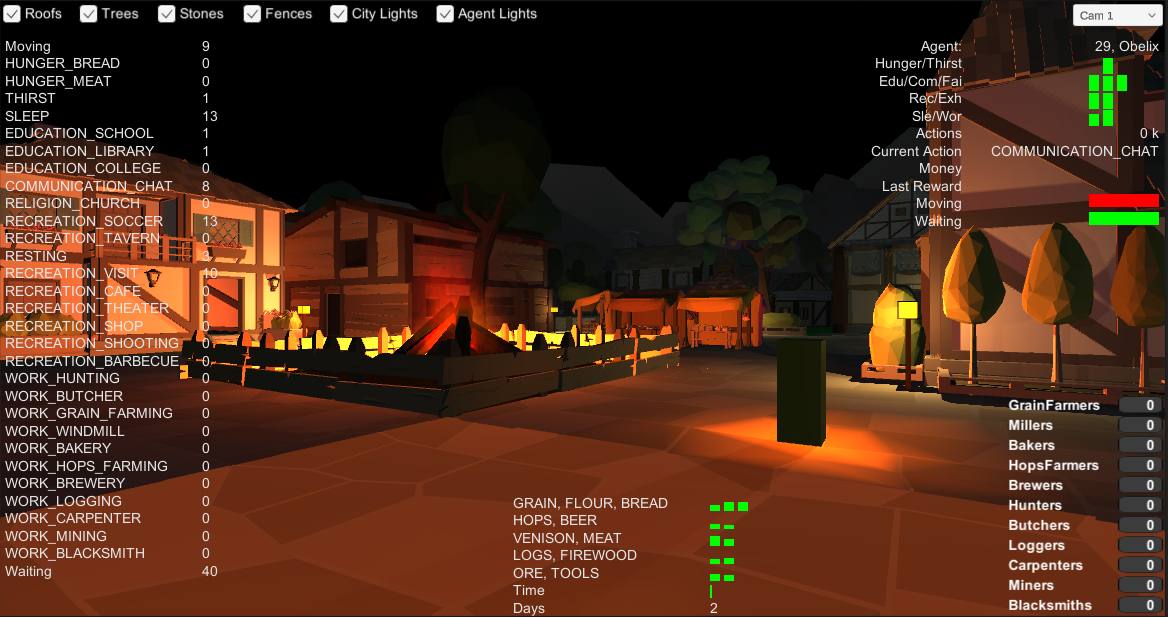
\includegraphics[scale=0.53]{images/village/village_ui_example_1.PNG}
\caption{UI aus Sicht eines Agenten}
\label{fig:village_ui_example_1}
\end{figure}

\paragraph{Anpassung der Szene}\label{szene_anpassung_ui}
Weiterhin wurden UI-Elemente entwickelt, um Anpassungen in der Szene vorzunehmen. Sämtliche Dächer der Gebäude im Dorf können über einen Agenten deaktiviert und aktiviert werden. Dadurch kann besser gesehen werden, wo die Agenten sich aufhalten. Zusätzlich können weitere Mesh-Elemente deaktiviert werden, um die Performance der Simulation zu erhöhen oder einen besseren Überblick zu bekommen. Konkret lässt sich das Mesh von Bäumen, Zäunen, Gebäuden und Felsen über einen Button deaktivieren. Zusätzlich können sämtliche Lichter in der Stadt deaktiviert werden. Dabei wird zwischen den Lichtquellen der Agenten und den Lichtquellen der Stadt unterschieden.
Weiterhin besteht die Möglichkeit, über einen Dropdown-Menü die Wahl der aktiven Kamera anzupassen. Dadurch kann ebenfalls die Spielerkamera aktiviert werden, sodass der \Fachbegriff{Player} gesteuert werden kann (siehe Abschnitt \ref{player}).
Diese Anpassungen werden in der Klasse \inlinecode{GameUI} vorgenommen. Die Klasse steuert die entsprechenden UI-Elemente bzw. nimmt Befehle von ihnen entgegen. Bei einer Verwendung mehrerer Dörfer wird nicht zwischen einzelnen Dörfern unterschieden. Die Änderungen treten stets für die gesamte Szene in Kraft. Die Komponente \inlinecode{GameUI} ist ein MonoBehavior und wird schon vor der Ausführung an ein GameObject angehängt. Innerhalb der Funktion \inlinecode{Start} werden Meshelemente und Lichtquellen innerhalb der Szene gesucht. Anschließend wird durch die Klasse \inlinecode{GameAcademy} die Funktion \inlinecode{initAgents} aufgerufen, nachdem die Initialisierung der Dörfer und Agenten abgeschlossen ist. Die Funktion \inlinecode{initAgents} bekommt eine Liste aller Agenten als Parameter und bezieht daraus deren Lichtquellen.


\subsection{Logging}\label{village_logging}
Für eine erleichterte Analyse der Simulation wird eine Menge von Daten mitgeschrieben. Informationen zu den Aktionen der Agenten werden gesammelt, die für die Auswertung der trainierten Policy relevant sind. Dabei werden keine Daten in Dateien geschrieben, sondern in Dictionaries gespeichert, die durch Debugging ausgelesen werden können. Neben den für die Darstellung im UI gesammelten Daten werden zusätzlich die Dauer von Aktionen sowie deren durchschnittliche Dauer mitgeschrieben (\inlinecode{VillageInfo.addActionDuration}). Außerdem werden die akkumulierten Belohnungen sowie die durchschnittlichen Belohnungen für getätigte Aktionen gespeichert (\inlinecode{ActionHandler.logReward}). Zusätzlich wird für alle Aktionen eine \inlinecode{Queue} gespeichert, sodass die letzten 100 konkreten Belohnungen abgefragt werden können. In der Klasse \inlinecode{VillageInfo} werden außerdem die durchschnittlichen Attribute der Agenten für die jeweiligen Aktionen gespeichert. Die \inlinecode{ActionMask}s können darüber hinaus nachvollzogen werden, indem sie im \inlinecode{ActionMaskingHandler} mitgeschrieben werden.

Um den Tagesablauf der Agenten anhand ihrer Bedürfnisse sichtbar zu machen, musste weiterhin ein Weg gefunden werden, die Bedürfnisse der Agenten zu bestimmten Zeitpunkten zu speichern. In der Klasse \inlinecode{Village} werden in der Funktion \inlinecode{updateTime} immer dann, wenn bestimmte zeitliche Thresholds überschritten wurden, die Bedürfnisse aller Agenten in einer verschachtelten Datenstruktur aus \inlinecode{List} und \inlinecode{Dictionary} hinterlegt. Durch die Nutzung eines Debuggers kann ein Schreibvorgang gestartet werden, der einen String aus der Datenstruktur erstellt und die enthaltenenen Daten in eine CSV-Datei schreibt. Dieser Vorgang wurde verwendet, um die im nachfolgenden Kapitel erkennbaren Abbildungen \ref{fig:reinforcement_needs_day_cycle} und \ref{fig:rulebased_day_cycle} zu erstellen. Die Granularität der Datenpunkte kann im \inlinecode{TimeController} durch eine Anpassung der Konstante \inlinecode{NEED\_LOG\_TIME\_INTERVAL} angepasst werden. Standardmäßig wurde der Wert so gewählt, dass nach jeweils zehn im Spiel vergangenen Minuten ein Logpunkt erstellt wird.

Das Logging kann in den Parametern der \inlinecode{GameAcademy} aktiviert werden (siehe Abschnitt \ref{gameacademy}).





\subsection{Fake Inference}\label{modes_fake_inference_etc}
Mit der Erhöhung des TimeScale-Faktors werden alle physikalische Vorgänge, die in der Engine beschrieben werden, ungenauer, da für jedes Update relativ gesehen mehr Zeit vergeht. Simuliert man beispielsweise den Wurf eines Balls und verzehnfacht die TimeScale, so werden während dieses Wurfes bei gleichbleibender Framerate nur ein Zehntel so häufig die Update-Funktionen aufgerufen.
Für die Navigation des Agenten über das NavMesh stellt dies ein essentielles Problem dar. Besonders die Navigation in engen Bereichen wird dadurch erschwert. Das hat zur Folge, dass NavMeshAgents mit steigender Timescale Türen verfehlen. Man stelle sich vor, dass ein Agent links von einer Tür steht und hindurch gehen möchte. Dazu muss er ein Stück weit nach rechts gehen. Wenn die Timescale zu hoch ist, so hat der Agent sich unter Umständen bereits beim Aufruf der nächsten Update-Funktion so weit nach rechts bewegt, dass er nun rechts von der Tür steht. Der Agent fängt nun an, zu oszillieren und schafft es nicht, die Tür zu durchschreiten. Durch eine Anpassung von Geschwindigkeit, Beschleunigung und Drehgeschwindigkeit kann dieses Phänomen nur bis zu einem bestimmten Grade unterbunden werden. Weiterhin wirken die Bewegungen der Agenten dann möglicherweise bei einer normalen Timescale falsch.

Aus diesem Grund wurde der sogenannte \Fachbegriff{Fake Inference}-Modus entwickelt, in dem keinerlei Bewegung der Agenten durch das NavMesh vorkommt. Die \inlinecode{MoveAction} agiert dann auf andere Weise und ruft nicht mehr den \inlinecode{MoveHandler} für die Navigation auf. Stattdessen wird die Zeit berechnet, die ein Agent normalerweise bei seiner durchschnittlichen Geschwindigkeit benötigen würde, um den Weg zu einem Ziel zu beschreiten. Mithilfe des NavMesh findet im \inlinecode{LocationHandler} die Berechnung des Pfades statt, den der NavMeshAgent normalerweise wählen würde. Diese Berechnung wurde in der Funktion \inlinecode{calculatePathLength} implementiert, die in Listing \ref{lst:calculate_path_length} zu erkennen ist.


\begin{minipage}{\linewidth}
\begin{lstlisting}[linewidth=16.4cm, label=lst:calculate_path_length, caption=Berechnung der Pfadlänge durch \inlinecode{calculatePathLength}, xleftmargin=1cm]
public IEnumerator calculatePathLength(Vector3 origin, Vector3 destination, NavMeshAgent navMeshAgent, int agentId) {
    yield return Ninja.JumpToUnity;
    NavMeshPath path = new NavMeshPath();
    navMeshAgent.CalculatePath(destination, path);
    yield return Ninja.JumpBack;

    float pathLength = 0f;
    Vector3[] wayPoints = new Vector3[path.corners.Length + 2];
    wayPoints[0] = origin;
    wayPoints[wayPoints.Length - 1] = destination;

    for (int i = 0; i < path.corners.Length; i++) {
        wayPoints[i + 1] = path.corners[i];
    }
    for (int i = 0; i < wayPoints.Length - 1; i++) {
        pathLength += Vector3.Distance(wayPoints[i], wayPoints[i + 1]);
    }
    _calculatedPathLengths[agentId] = pathLength;
    yield return null;
}
\end{lstlisting}
\end{minipage}

Hierfür muss eine Coroutine verwendet werden, da die Berechnung eines Pfades über das NavMesh kein unmittelbares Ergebnis liefert. Die Funktionen \inlinecode{Ninja.JumpToUnity} und \inlinecode{Ninja.JumpBack} aus der \Fachbegriff{Thread Ninja}-Bibliothek \cite{ninja} müssen verwendet werden, da in C\#-Coroutinen normalerweise kein Unity-Code verwendet werden können. Durch diese Anweisung findet ein Sprung aus dem Thread heraus in den Unity-Kontext und wieder zurück statt.
\inlinecode{navMeshAgent.CalculatePath} berechnet dann den eigentlichen Pfad mit dem Typen \inlinecode{NavMeshPath}. Alle Wegpunkte des Pfades inklusive dem Start- und Zielort werden anschließend in ein Array geschrieben. Anschließend wird für jeden Wegpunkt die jeweilige Distanz zum nächsten Wegpunkt durch \inlinecode{Vector3.Distance} ermittelt und in einer Variablen aufaddiert. Da kein anderer Wert als \inlinecode{IEnumerator} zurückgegeben werden kann, wird das Ergebnis in \inlinecode{\_calculatedPathLengths} gespeichert und kann anschließend durch die Funktion \inlinecode{getCalculatedPathLength} abgerufen werden.

In der \inlinecode{GameAcademy} kann festgelegt werden, ob der normale Inference-Modus oder der Fake Inference-Modus verwendet werden soll. Entsprechend ändert sich der in der statischen Variable \inlinecode{GameAcademy.GAME\_MODE} festgelegte Spielmodus. Dieser Wert wird in der Klasse \inlinecode{MoveAction} geprüft. Dafür werden die Methoden \inlinecode{\_handleInference} und \inlinecode{\_handleFakeInference} gebraucht. Diese wird im Listing \ref{lst:moveaction_fakeinference} beschrieben.

\begin{minipage}{\linewidth}
\begin{lstlisting}[linewidth=16.4cm, label=lst:moveaction_fakeinference, caption=Behandlung der Fake Inference in der Klasse \inlinecode{MoveAction}, xleftmargin=1cm]
private IEnumerator _handleFakeInference(Vector3 destination) {
    yield return _moveHandler.StartCoroutine(_locationHandler.calculatePathLength(_npc.transform.position, destination, _moveHandler.NavAgent, _npc.AgentId));
    float pathLength = _locationHandler.getCalculatedPathLength(_npc.AgentId);
    float speed = _moveHandler.NavAgent.speed;
    if (pathLength < 1f) _duration = 1f;
    else _duration = (pathLength / speed) * PATH_LENGTH_DURATION_MULTIPLIER;

    _npc.transform.position = destination;

    WaitAction waitAction = new WaitAction(_actionType, _npc, _duration);
    _npc.StartCoroutine(waitAction.execute(_finishedMoving, _cancelCallback));
}
\end{lstlisting}
\end{minipage}

Im Fake Inference-Modus wird zunächst die Länge des Pfades ermittelt, wie bereits oben beschrieben. Schließlich wird die Länge des Pfades durch die Maximalgeschwindigkeit des Agenten geteilt, um die ideal nötige Dauer zu erhalten. Diese wird mit einem Faktor multipliziert, der empirisch ermittelt wurde und mit ausreichender Genauigkeit ähnliche Ergebnisse liefert, wie durch die tatsächliche Navigation eines NavMeshAgent. Der Agent wird anschließend zum Zielort teleportiert. Die berechnete Dauer, die eine Navigation zum Zielort in Anspruch nehmen würde, wird nun genutzt, um stattdessen eine \inlinecode{WaitAction} zu erzeugen. Der Agent wartet also so lange, wie die Aktion normalerweise benötigen würde.
Da die Navigation der Agenten zum Ziel lediglich aus visuellen Gründen nötig ist, stellt dieses Verfahren einen legitimen Ersatz dar und beeinflusst nicht die Entscheidungsfindung des Agenten.

\paragraph{Nutzung des Fake Inference-Verfahrens für den Trainingsfall}
Das gleiche Verfahren wird ebenfalls für das Training des Agenten angewendet, da hier mit sehr hohen TimeScale-Faktoren gearbeitet wird, um möglichst schnell Ergebnisse zu erhalten. Im Trainingsmodus wird dann ebenfalls die Funktion \inlinecode{\_handleFakeInference} aufgerufen.
Eine Ausnahme besteht jedoch, wenn mit lediglich einem einzelnen Agenten gearbeitet wird. Normalerweise regelt der \inlinecode{TimeController} das Voranschreiten der Zeit durch den Aufruf einer \inlinecode{Update}-Funktion. Wenn nur ein Agent verwendet wird, kann eine drastische Beschleunigung erzielt werden, indem der Agent selbst die Zeit voranschreiten lässt. Wie bei der Fake Inference wird jede \inlinecode{MoveAction} des Agenten in eine \inlinecode{WaitAction} umgewandelt, die auf der Länge des theoretischen Pfades basiert. Anstatt zu warten, werden alle \inlinecode{WaitAction}s des Agenten allerdings direkt übersprungen. Der Zeit des \inlinecode{TimeController}s schreitet äquivalent zur Dauer der \inlinecode{WaitAction} voran. Dadurch muss nicht auf die \inlinecode{WaitAction} gewartet werden und der \inlinecode{TimeController} berechnet trotzdem korrekte Werte für die Bedürfnisse des Agenten, die nun für die Observations einer neuen Entscheidung genutzt werden können.
Anstatt Aktionen auszuführen, werden diese übersprungen und die Zeit wird künstlich vorgespult, um sofort eine weitere Aktion auszuführen. Dadurch wird der Intervall zwischen der Ausführung von Aktionen extrem verringert. Der große Nachteil dieser Methode ist jedoch, dass nur ein einzelner Agent verwendet werden kann, da mehrere Agenten schon nach der ersten Aktion nicht mehr synchron zueinander wären bzw. die Zeit zu weit voranschreiten lassen würden. Jeder Agent bräuchte dann seinen eigenen \inlinecode{TimeController}, was den Sinn einer Dorfgemeinschaft zunichte machen würde.


\subsection{Player}\label{player}
Um die erreichte Immersion der Simulation zu beurteilen, wurde ein einfacher spielbarer Charakter implementiert. Für dessen Steuerung wird eine Instanz der bereits in Unity vorhandenen Klasse \inlinecode{CharacterController} genutzt, die die Bewegung eines Charakters erlaubt. Dafür werden Tastatureingaben genutzt, die dem \inlinecode{CharacterController} zur Verfügung gestellt werden müssen. Dafür wird die Klasse \inlinecode{PlayerController} verwendet. Die Implementierung der Klasse ist in Listing \ref{lst:player_controller} zu sehen.

\begin{minipage}{\linewidth}
\begin{lstlisting}[linewidth=16.4cm, label=lst:player_controller, caption=Implementierung des \inlinecode{PlayerController}, xleftmargin=1cm]
public class PlayerController : MonoBehaviour {
    public CharacterController characterController;
    private float _lastYPos;

    private void Start() {
        characterController.detectCollisions = true;
        _lastYPos = transform.position.y;
    }

    private void Update() {
        float moveInput = Input.GetAxis("Vertical");
        float turnInput = Input.GetAxis("Horizontal");
        float currentYPos = transform.position.y;
        bool alreadyJumping = !Mathf.Approximately(_lastYPos, currentYPos);

        float moveSpeed = 0.25f;
        if (Input.GetKey(KeyCode.LeftShift)) moveSpeed = 0.65f;
        else if (Input.GetKey(KeyCode.LeftAlt)) moveSpeed = 0.1f;

        Vector3 move = transform.TransformDirection(Vector3.forward * moveInput * moveSpeed);
        if (Input.GetKey(KeyCode.Space) && !alreadyJumping) move.y = 4f;
        else move.y -= 9.81f * Time.deltaTime;

        characterController.Move(move);
        transform.Rotate(0, turnInput * 2.5f, 0);
        _lastYPos = currentYPos;
    }
}
\end{lstlisting}
\end{minipage}

Die Inputs werden kontinuierlich in der Funktion \inlinecode{Update} durch eine Abfrage von \inlinecode{Input.GetAxis("Vertical")} und \inlinecode{Input.GetAxis("Horizontal")} geprüft und dem \inlinecode{CharacterController} zur Verfügung gestellt, um den Spieler zu bewegen. Die verwendeten Achsen und die mit ihnen assoziierten Eingabetasten können im \Fachbegriff{Input}-Fenster in den Projekteinstellungen des Unity-Editors verändert werden. Klassischerweise werden die Tasten \textit{W}, \textit{A}, \textit{S} und \textit{D} verwendet. Zusätzlich werden die Tasten \textit{Alt}, \textit{Shift} und \textit{Space} genutzt, um den Spieler langsamer oder schneller laufen zu lassen bzw. einen Sprung auszuführen.

Aus den einzelnen Inputs wird ein Vektor konstruiert, der die Bewegung des Charakters durch \inlinecode{characterController.Move(move)} herbeiführt. Weiterhin wird der Spieler durch \inlinecode{transform.Rotate(0, turnInput * 2.5f, 0)} gedreht.








\section{Start und Bedienung der Dorfsimulation}
Für die Nutzung der Simulation muss Unity installiert werden \cite{unity_download}. Eine der Versionen \textit{2019.2.x} ist zwingend erforderlich. Idealerweise sollte die Version \textit{2019.2.8f1} verwendet werden - für alle weiteren Versionen \textit{2019.2.x} wird ansonsten eine automatische Migration des Projekts durch Unity durchgeführt. Im Rahmen dieser Thesis wurde eine Migration des Projektes nicht überprüft oder getestet, sodass Nebenerscheinungen auftreten können. Das Projekt, das die Simulation beinhaltet, ist auf dem mitgelieferten Speichermedium oder im entsprechenden GitHub-Repository zu finden \cite{thesis_github_project}.
Für die Einstellung bestimmter Features wie dem NavMesh muss Unity Pro installiert sein. Diese Features können auch mit der normalen Version verwendet, aber nicht verändert werden.
Die wichtigsten Parameter zur Einstellung der Simulation (siehe Abschnitt \ref{tab:game_academy_parameters}) können in der \inlinecode{GameAcademy} angepasst werden, die in einem GameObject mit dem Titel \Fachbegriff{Academy} als Komponente zu finden ist. Weiterhin können den Agenten und das Dorf betreffende Einstellungen in Prefabs mit den Namen \Fachbegriff{Agent} und \Fachbegriff{Village} angepasst werden. Dafür werden die Komponenten \inlinecode{NpcAgent} und \inlinecode{Village} verwendet.


